\documentclass[12pt,a4paper,oneside]{report}
\usepackage[T1]{fontenc}
\usepackage[utf8]{inputenc}
\DeclareUnicodeCharacter{1D49}{\textsuperscript{e}}
\usepackage[french]{babel}
\usepackage{lmodern}
\usepackage{microtype}
\usepackage{geometry}
\geometry{left=3cm,right=2.5cm,top=2.5cm,bottom=2.5cm}
\usepackage{setspace}\onehalfspacing
\usepackage{graphicx}\usepackage{float}
\usepackage{booktabs,longtable,array}
\usepackage{calc}
\usepackage{amsmath,amssymb}
\usepackage{enumitem}
\usepackage{hyperref}\hypersetup{hidelinks}
\usepackage{url}\usepackage{caption}
\usepackage{csquotes}
\usepackage[backend=biber,style=ieee,sorting=none]{biblatex}
\addbibresource{references.bib}\usepackage{titlesec}\usepackage{fancyhdr}
\pagestyle{fancy}\fancyhf{}\fancyhead[R]{\thepage}\setlength{\headheight}{14.5pt}
\setcounter{secnumdepth}{3}\setcounter{tocdepth}{3}
\renewcommand{\contentsname}{Table des matières}
\renewcommand{\listfigurename}{Liste des figures}
\renewcommand{\listtablename}{Liste des tableaux}
\renewcommand{\bibname}{Références bibliographiques}
\begin{document}
\begin{titlepage}\centering\vspace*{2cm}
{\Large\textbf{TRAVAIL DE FIN DE CYCLE}\par}\vspace{2cm}
{\LARGE\textbf{Jumeau numérique intégrant l'intelligence artificielle}\par}\vspace{1cm}
{\large Version LaTeX issue du document source fourni\par}\vfill
{\large Auteur : à compléter\par}{\large Institution : à compléter\par}{\large Année académique : 2025--2026\par}
\end{titlepage}
\pagenumbering{roman}\tableofcontents\listoffigures\listoftables\clearpage\pagenumbering{arabic}


\chapter*{INTRODUCTION}\addcontentsline{toc}{chapter}{INTRODUCTION}\label{introduction}

\subsection{1. CONTEXTE GÉNÉRAL DE
L\textquotesingle ÉTUDE}\label{contexte-guxe9nuxe9ral-de-luxe9tude}

Selon le rapport conjoint de l\textquotesingle Organisation mondiale de
la Santé (OMS) et du Fonds des Nations Unies pour
l\textquotesingle enfance (UNICEF), publié dans le cadre du Joint
Monitoring Programme (JMP), près de 2,2 milliards de personnes dans le
monde ne disposaient pas, en 2022, d\textquotesingle un service
d\textquotesingle eau potable géré en toute sécurité, tandis que 703
millions de personnes ne bénéficiaient même pas d\textquotesingle un
service de base d\textquotesingle approvisionnement en eau potable
\cite{ref1}. Ces statistiques démontrent que, malgré les progrès enregistrés
au cours des dernières décennies, l\textquotesingle accès universel à
une eau potable de qualité demeure un défi majeur pour la communauté
internationale et constitue l\textquotesingle un des objectifs
prioritaires de l\textquotesingle Objectif de Développement Durable n°6
(ODD 6), qui vise à garantir l\textquotesingle accès de tous à
l\textquotesingle eau potable et à l\textquotesingle assainissement
d\textquotesingle ici 2030 \cite{ref2}.

L\textquotesingle eau potable représente l\textquotesingle une des
ressources naturelles les plus essentielles à la survie humaine et au
développement des sociétés modernes. Elle joue un rôle fondamental non
seulement dans la consommation domestique, mais également dans les
domaines de la santé publique, de l\textquotesingle agriculture, de
l\textquotesingle industrie, de l\textquotesingle assainissement et du
développement économique. Depuis plusieurs décennies, la communauté
internationale considère l\textquotesingle accès à l\textquotesingle eau
potable comme un facteur déterminant de la qualité de vie et un
indicateur majeur du niveau de développement d\textquotesingle une
nation. La disponibilité d\textquotesingle une eau potable sûre et
accessible contribue directement à la réduction des maladies hydriques,
à l\textquotesingle amélioration des conditions sanitaires et au
renforcement du bien-être social des populations. En raison de cette
importance capitale, les institutions internationales ont
progressivement reconnu l\textquotesingle accès à l\textquotesingle eau
potable comme un droit humain fondamental nécessitant une gestion
durable et efficace des infrastructures hydrauliques \cite{ref3}.

Malgré son importance, l\textquotesingle accès à l\textquotesingle eau
potable demeure un défi majeur dans plusieurs régions du monde,
particulièrement dans les pays en développement. La croissance
démographique rapide, l\textquotesingle urbanisation non planifiée, les
changements climatiques, la vétusté des infrastructures ainsi que
l\textquotesingle insuffisance des investissements dans les systèmes
hydrauliques aggravent les difficultés liées à la distribution de
l\textquotesingle eau potable. Selon les rapports de
l\textquotesingle Organisation mondiale de la Santé (OMS), du Programme
conjoint OMS/UNICEF (JMP) et de la Banque mondiale, plusieurs millions
de personnes continuent de faire face à un accès limité ou irrégulier à
une eau potable sécurisée. Le rapport JMP 2023 indique notamment que 2,2
milliards de personnes ne disposent toujours pas d\textquotesingle un
service d\textquotesingle eau potable géré en toute sécurité, tandis que
la Banque mondiale souligne que les insuffisances des infrastructures
hydrauliques et les faibles performances des services
d\textquotesingle eau entraînent chaque année
d\textquotesingle importantes pertes économiques dans les pays à revenu
faible et intermédiaire \cite{ref1}, \cite{ref4}, \cite{ref5}. Les interruptions
fréquentes des services, les pertes importantes d\textquotesingle eau
causées par les fuites dans les réseaux de distribution et le manque de
surveillance efficace constituent autant de défis techniques et
organisationnels auxquels les gestionnaires des réseaux hydrauliques
doivent faire face.

Dans les infrastructures modernes de distribution d\textquotesingle eau,
la problématique des pertes techniques demeure particulièrement
préoccupante. Les réseaux de distribution traditionnels souffrent
souvent d\textquotesingle un manque de mécanismes intelligents
permettant une surveillance en temps réel des paramètres essentiels tels
que la pression, le débit, la qualité de l\textquotesingle eau ou encore
l\textquotesingle état des conduites. Cette insuffisance réduit
considérablement la capacité des opérateurs à détecter rapidement les
anomalies, à prévoir les pannes ou à optimiser les opérations de
maintenance. Ainsi, de nombreuses villes enregistrent des volumes
importants d\textquotesingle eau non facturée, résultant principalement
des fuites invisibles, des ruptures de conduites et des inefficacités
opérationnelles. L\textquotesingle eau non facturée (\emph{Non-Revenue
Water -- NRW}) désigne, selon l\textquotesingle International Water
Association (IWA), la différence entre le volume d\textquotesingle eau
introduit dans le réseau de distribution et le volume effectivement
facturé aux consommateurs. Elle comprend les pertes réelles (fuites sur
les conduites et les réservoirs), les pertes apparentes (fraudes,
erreurs de comptage) ainsi que les consommations autorisées mais non
facturées. Cet indicateur est aujourd\textquotesingle hui largement
utilisé pour évaluer la performance technique et économique des réseaux
d\textquotesingle eau potable \cite{ref6}. Dans ce contexte, la
modernisation des systèmes de gestion de l\textquotesingle eau apparaît
aujourd\textquotesingle hui comme une nécessité incontournable afin
d\textquotesingle améliorer la performance des réseaux et
d\textquotesingle assurer une meilleure continuité des services.

Par ailleurs, les progrès technologiques observés au cours des dernières
décennies ouvrent de nouvelles perspectives pour la gestion intelligente
des infrastructures urbaines. L\textquotesingle intégration des
technologies numériques, notamment l\textquotesingle Internet des objets
(Internet of Things -- IoT), qui permet la collecte automatique des
données grâce à des capteurs connectés, les systèmes cyber-physiques
(Cyber-Physical Systems -- CPS), qui assurent
l\textquotesingle interaction entre les équipements physiques et les
systèmes informatiques, les technologies Big Data, destinées au stockage
et à l\textquotesingle analyse de grands volumes de données, ainsi que
l\textquotesingle intelligence artificielle (IA), capable
d\textquotesingle exploiter ces données afin de détecter des anomalies,
prédire des défaillances et assister la prise de décision, permet
désormais d\textquotesingle améliorer considérablement la surveillance
et l\textquotesingle optimisation des systèmes complexes. Ces
innovations technologiques rendent possible la collecte en temps réel
des données opérationnelles, leur traitement automatisé ainsi que la
génération de prédictions utiles à la prise de décision. Dans le domaine
de la gestion de l\textquotesingle eau, ces technologies contribuent
progressivement à transformer les réseaux conventionnels en
infrastructures intelligentes capables de réagir rapidement face aux
anomalies et de s\textquotesingle adapter aux variations de la demande.
Ces différents concepts seront développés de manière approfondie dans la
revue de littérature du présent mémoire \cite{ref7}.

Parmi les innovations technologiques les plus prometteuses figure le
concept de jumeau numérique (\emph{Digital Twin}), qui consiste à créer
une représentation virtuelle dynamique d\textquotesingle un système
physique réel à partir de données collectées en continu. Introduit par
Michael Grieves dans le domaine de la gestion du cycle de vie des
produits (\emph{Product Lifecycle Management -- PLM}), le concept de
jumeau numérique est aujourd\textquotesingle hui considéré comme
l\textquotesingle une des technologies les plus prometteuses de
l\textquotesingle industrie 4.0 et des villes intelligentes \cite{ref8}.
Cette technologie permet de simuler le comportement d\textquotesingle un
réseau, d\textquotesingle évaluer différents scénarios de
fonctionnement, d\textquotesingle anticiper les dysfonctionnements et de
proposer des solutions optimales avant même qu\textquotesingle un
problème ne survienne. Couplé à l\textquotesingle intelligence
artificielle, le jumeau numérique devient un outil stratégique
permettant non seulement de surveiller les infrastructures en temps
réel, mais aussi d\textquotesingle effectuer des analyses prédictives
capables d\textquotesingle optimiser la maintenance et les performances
globales d\textquotesingle un réseau \cite{ref9}. Son utilisation dans le
domaine de la gestion de l\textquotesingle eau représente
aujourd\textquotesingle hui une avancée majeure vers des villes
intelligentes (\emph{Smart Cities}) plus résilientes et plus efficaces.

\subsection{2. PROBLÉMATIQUE}\label{probluxe9matique}

L\textquotesingle accès à l\textquotesingle eau potable constitue
l\textquotesingle un des principaux défis de développement auxquels sont
confrontées plusieurs villes des pays en développement, particulièrement
en Afrique subsaharienne. \textbf{Selon le Programme commun OMS/UNICEF
(JMP), l\textquotesingle Afrique subsaharienne demeure la région où la
proportion de populations ne bénéficiant pas d\textquotesingle un
service d\textquotesingle eau potable géré en toute sécurité est la plus
élevée au monde. Des métropoles telles que Kinshasa (République
Démocratique du Congo), Lagos (Nigéria), Nairobi (Kenya) ou encore Dakar
(Sénégal) font face à une croissance démographique rapide qui exerce une
pression considérable sur les infrastructures hydrauliques existantes}
\cite{ref1}\textbf{,} \cite{ref10}\textbf{.} Bien que cette ressource soit
essentielle à la santé publique, au bien-être social et au développement
économique, les infrastructures de distribution d\textquotesingle eau
demeurent souvent confrontées à de nombreuses insuffisances techniques,
organisationnelles et technologiques. Dans plusieurs centres urbains,
les systèmes de distribution d\textquotesingle eau sont caractérisés par
une croissance insuffisamment maîtrisée des infrastructures, un
vieillissement progressif des conduites, une maintenance essentiellement
corrective ainsi qu\textquotesingle une faible capacité de surveillance
continue du réseau \cite{ref11}. Cette situation affecte considérablement
l\textquotesingle efficacité des services de distribution
d\textquotesingle eau et expose les populations à des difficultés
récurrentes d\textquotesingle approvisionnement.

En République Démocratique du Congo, et particulièrement dans les
centres urbains à forte croissance démographique, les réseaux de
distribution d\textquotesingle eau potable subissent une pression
croissante résultant de l\textquotesingle augmentation rapide de la
population, de l\textquotesingle expansion urbaine désordonnée et des
contraintes liées à la modernisation des infrastructures publiques.
Malgré les efforts fournis par les structures de gestion
d\textquotesingle eau potable, plusieurs villes continuent à faire face
à des interruptions fréquentes du service, à une distribution
irrégulière de l\textquotesingle eau, à des pertes importantes causées
par les fuites invisibles ainsi qu\textquotesingle à des difficultés de
maintenance des infrastructures existantes \cite{ref12}. \textbf{Les
rapports publiés par la REGIDESO, le Ministère des Ressources
Hydrauliques et Électricité ainsi que le Programme des Nations Unies
pour le Développement (PNUD-RDC) soulignent que les besoins en
investissements dans les infrastructures hydrauliques demeurent
importants afin d\textquotesingle améliorer durablement le taux de
desserte en eau potable et la qualité du service dans les principaux
centres urbains du pays} \cite{ref13}\textbf{,} \cite{ref14}\textbf{,}
\cite{ref15}\textbf{.}

La ville de Bukavu n\textquotesingle échappe pas à cette réalité. Avec
l\textquotesingle accroissement continu de la population,
l\textquotesingle extension rapide des quartiers périphériques et
l\textquotesingle augmentation progressive des besoins en eau potable,
le réseau de distribution existant se retrouve confronté à des défis
majeurs de performance et de gestion. Plusieurs ménages connaissent
régulièrement des perturbations dans l\textquotesingle approvisionnement
en eau, tandis que certaines zones demeurent insuffisamment desservies.
À cela s\textquotesingle ajoutent les difficultés liées à la détection
rapide des anomalies techniques telles que les baisses de pression, les
ruptures de conduites, les fuites non détectées ou encore les
dysfonctionnements des équipements de pompage. Ces problèmes
occasionnent non seulement des pertes importantes d\textquotesingle eau,
mais aussi une augmentation des coûts d\textquotesingle exploitation et
une réduction de la qualité du service offert à la population \cite{ref16}.
\textbf{Selon les données publiées par la REGIDESO Sud-Kivu, complétées
par les observations réalisées lors de la phase exploratoire de cette
étude, certains quartiers de la commune de Kadutu connaissent des
interruptions récurrentes de la desserte en eau potable,
particulièrement durant les périodes de forte demande. Bien que les
données détaillées sur le volume réel des pertes ou le taux exact de
desserte restent limitées, ces constats mettent en évidence la nécessité
de disposer d\textquotesingle outils permettant une surveillance plus
efficace du réseau et une meilleure anticipation des défaillances.}

\textbf{De plus}, les méthodes conventionnelles de gestion du réseau
d\textquotesingle eau reposent encore largement sur des interventions
manuelles, des inspections périodiques et des approches réactives de
maintenance. Dans ce modèle traditionnel, les équipes techniques
interviennent souvent après l\textquotesingle apparition visible
d\textquotesingle une panne ou d\textquotesingle une anomalie, ce qui
entraîne des retards d\textquotesingle intervention et accentue les
pertes techniques. En outre, l\textquotesingle absence de systèmes
avancés de surveillance en temps réel limite fortement la capacité des
gestionnaires à anticiper les dysfonctionnements ou à prendre des
décisions optimales concernant l\textquotesingle exploitation du réseau
\cite{ref6}. Cette situation met en évidence les limites des approches
classiques face à la complexité croissante des systèmes urbains
modernes.

\textbf{Dans ce contexte}, plusieurs travaux scientifiques montrent que
l\textquotesingle intégration des technologies numériques, notamment
l\textquotesingle Internet des objets (IoT),
l\textquotesingle intelligence artificielle et le \textbf{jumeau
numérique} (\emph{Digital Twin}), constitue aujourd\textquotesingle hui
une approche prometteuse pour améliorer la gestion des infrastructures
hydrauliques. Des expériences menées en Europe et en Asie ont démontré
que ces technologies permettent d\textquotesingle assurer une
surveillance en temps réel des réseaux, de détecter plus rapidement les
anomalies, de prévoir certaines défaillances et
d\textquotesingle optimiser les opérations de maintenance \cite{ref9},
\cite{ref17}. \textbf{En Afrique subsaharienne, quelques initiatives
commencent également à émerger. Par exemple, des travaux portant sur les
réseaux d\textquotesingle eau intelligents au Kenya, en Afrique du Sud
et au Rwanda ont exploré l\textquotesingle utilisation de capteurs
connectés, de plateformes IoT et d\textquotesingle algorithmes
d\textquotesingle analyse de données pour améliorer la gestion des
services d\textquotesingle eau, même si l\textquotesingle utilisation
complète du concept de jumeau numérique demeure encore limitée}
\cite{ref18}\textbf{,} \cite{ref19}\textbf{.} En République Démocratique du
Congo, et plus particulièrement dans la ville de Bukavu,
l\textquotesingle application de ces technologies reste encore
embryonnaire, ce qui met en évidence une réelle opportunité de
recherche.

C\textquotesingle est dans cette perspective que la présente étude
envisage d\textquotesingle explorer le potentiel d\textquotesingle un
\textbf{jumeau numérique intégrant des techniques
d\textquotesingle intelligence artificielle} afin de contribuer à
l\textquotesingle optimisation du déploiement, de la surveillance et de
la maintenance du réseau de fourniture d\textquotesingle eau potable de
la commune de Kadutu.

Dès lors, la présente étude cherche à répondre à la question
fondamentale suivante :

\textbf{Comment la conception et le développement d\textquotesingle un
jumeau numérique intégrant l\textquotesingle intelligence artificielle
peuvent-ils contribuer à optimiser le déploiement, la surveillance et la
maintenance du réseau de fourniture d\textquotesingle eau potable de la
commune de Kadutu ?}

\subsection{3. HYPOTHÈSES DE
RECHERCHE}\label{hypothuxe8ses-de-recherche}

\subsubsection{3.1. Hypothèse
générale}\label{hypothuxe8se-guxe9nuxe9rale}

La mise en œuvre d\textquotesingle un \textbf{jumeau numérique intégrant
des techniques d\textquotesingle intelligence artificielle} devrait
permettre d\textquotesingle améliorer significativement les performances
du réseau de fourniture d\textquotesingle eau potable de la commune de
\textbf{Kadutu} en réduisant les pertes d\textquotesingle eau, en
améliorant la rapidité de détection des anomalies et en optimisant les
opérations de maintenance grâce à l\textquotesingle exploitation en
temps réel des données issues des capteurs intelligents. Cette
amélioration devrait se traduire par une diminution des délais
d\textquotesingle intervention, une meilleure disponibilité du réseau
ainsi qu\textquotesingle une optimisation de la gestion des
infrastructures hydrauliques par rapport aux méthodes conventionnelles
de surveillance et de maintenance.

Cette hypothèse repose sur le principe selon lequel les technologies
émergentes, notamment les capteurs intelligents, les systèmes de
modélisation numérique, les plateformes de l\textquotesingle Internet
des objets (Internet of Things -- IoT) ainsi que les techniques
d\textquotesingle intelligence artificielle appliquées aux réseaux
hydrauliques intelligents, permettent d\textquotesingle améliorer
l\textquotesingle efficacité opérationnelle des infrastructures en
favorisant une gestion proactive, prédictive et basée sur les données
\cite{ref20}.

\subsubsection{3.2. Hypothèses
spécifiques}\label{hypothuxe8ses-spuxe9cifiques}

Afin d\textquotesingle apporter une réponse détaillée à la problématique
de recherche, les hypothèses spécifiques suivantes sont formulées :

\subsubsection{Première hypothèse
spécifique}\label{premiuxe8re-hypothuxe8se-spuxe9cifique}

La modélisation numérique du réseau de distribution
d\textquotesingle eau potable de la commune de \textbf{Kadutu}
permettrait de représenter virtuellement le comportement du système
physique afin de faciliter la surveillance, la simulation des scénarios
de fonctionnement et l\textquotesingle analyse des performances du
réseau.

Cette hypothèse suppose qu\textquotesingle une représentation numérique
dynamique du réseau peut améliorer la compréhension des interactions
entre les différents composants du système hydraulique, notamment les
conduites, les réservoirs, les stations de pompage et les points de
distribution \cite{ref8}. Elle devrait également permettre
d\textquotesingle actualiser automatiquement l\textquotesingle état du
réseau à partir des données collectées par les capteurs intelligents et
de simuler différents scénarios de fonctionnement afin
d\textquotesingle anticiper les dysfonctionnements potentiels.

\subsubsection{Deuxième hypothèse
spécifique}\label{deuxiuxe8me-hypothuxe8se-spuxe9cifique}

L\textquotesingle intégration des données issues des capteurs
intelligents (pression, débit, qualité de l\textquotesingle eau, niveau
des réservoirs et détection des fuites) permettrait
d\textquotesingle assurer une surveillance continue et en temps réel du
réseau de distribution d\textquotesingle eau potable.

Cette hypothèse s\textquotesingle appuie sur le fait que les
technologies de l\textquotesingle Internet des objets (Internet of
Things -- IoT) facilitent la collecte automatique et continue des
données opérationnelles, améliorant ainsi la rapidité de détection des
anomalies techniques. Il est supposé que les informations issues des
capteurs pourront être transmises à intervalles réguliers vers le jumeau
numérique afin d\textquotesingle assurer une actualisation permanente de
l\textquotesingle état du réseau et une meilleure réactivité des
gestionnaires \cite{ref7}.

\subsubsection{Troisième hypothèse
spécifique}\label{troisiuxe8me-hypothuxe8se-spuxe9cifique}

L\textquotesingle utilisation de techniques
d\textquotesingle intelligence artificielle dans
l\textquotesingle analyse des données du réseau permettrait de détecter
automatiquement les anomalies, de prévoir certaines défaillances
techniques et d\textquotesingle optimiser les opérations de maintenance
avant l\textquotesingle apparition des pannes majeures.

Cette hypothèse repose sur les capacités des techniques
d\textquotesingle apprentissage automatique (\emph{Machine Learning}),
notamment l\textquotesingle apprentissage supervisé et les algorithmes
de classification et de régression, à exploiter les données historiques
et les données collectées en temps réel afin
d\textquotesingle identifier des comportements anormaux,
d\textquotesingle effectuer des analyses prédictives et de recommander
des actions correctives adaptées \cite{ref21}.

\subsubsection{Quatrième hypothèse
spécifique}\label{quatriuxe8me-hypothuxe8se-spuxe9cifique}

La mise en œuvre d\textquotesingle une plateforme intelligente basée sur
un \textbf{jumeau numérique} pourrait contribuer à réduire les pertes
d\textquotesingle eau grâce à une surveillance continue du réseau et à
une détection précoce des anomalies.

Ajoutons que, cette plateforme permettrait d\textquotesingle améliorer
la réactivité des équipes techniques lors des opérations de maintenance
et de faciliter la planification du déploiement du réseau vers les
nouvelles zones urbaines en fournissant des informations fiables et
actualisées pour la prise de décision. Cette hypothèse considère que
l\textquotesingle automatisation des mécanismes de surveillance,
d\textquotesingle analyse et d\textquotesingle aide à la décision
constitue un levier essentiel pour moderniser les systèmes publics de
distribution d\textquotesingle eau potable dans les villes à forte
croissance démographique \cite{ref17}.

\subsection{4. OBJECTIFS DE
L\textquotesingle ÉTUDE}\label{objectifs-de-luxe9tude}

\subsubsection{4.1. Objectif général}\label{objectif-guxe9nuxe9ral}

L\textquotesingle objectif général de cette étude est de
\textbf{concevoir et de développer un jumeau numérique intégrant
l\textquotesingle intelligence artificielle} destiné à optimiser le
déploiement, la surveillance et la maintenance du réseau de fourniture
d\textquotesingle eau potable de la commune de Kadutu. À travers cette
conception, l\textquotesingle étude vise à proposer une solution
numérique innovante susceptible d\textquotesingle améliorer la gestion
des infrastructures hydrauliques, de contribuer à la réduction des
pertes d\textquotesingle eau et de renforcer
l\textquotesingle efficacité du service de distribution
d\textquotesingle eau potable.

Cet objectif général s\textquotesingle inscrit dans une logique de
modernisation des systèmes de gestion de l\textquotesingle eau potable
par l\textquotesingle utilisation des technologies numériques
intelligentes capables de collecter, d\textquotesingle analyser et
d\textquotesingle exploiter les données du réseau afin
d\textquotesingle améliorer la prise de décision, la planification des
interventions et la maintenance des infrastructures hydrauliques
\cite{ref17}.

\subsubsection{4.2. Objectifs
spécifiques}\label{objectifs-spuxe9cifiques}

Afin d\textquotesingle atteindre l\textquotesingle objectif général
ci-dessus défini, la présente étude poursuit les objectifs spécifiques
suivants :

\subsubsection{4.2.1. Analyser le fonctionnement du réseau de fourniture
d\textquotesingle eau potable de la ville de
Bukavu}\label{analyser-le-fonctionnement-du-ruxe9seau-de-fourniture-deau-potable-de-la-ville-de-bukavu}

Il s\textquotesingle agira d\textquotesingle étudier le système actuel
de distribution d\textquotesingle eau potable afin
d\textquotesingle identifier ses principales caractéristiques, ses
composantes techniques, ses contraintes de fonctionnement ainsi que les
problèmes liés aux fuites, aux pannes, aux interruptions de service et
aux difficultés de maintenance. \textbf{Cette analyse reposera sur
l\textquotesingle exploitation des documents techniques disponibles, des
données d\textquotesingle exploitation fournies par la REGIDESO, des
entretiens avec les responsables techniques ainsi que des observations
réalisées sur le terrain, dans la mesure où ces informations seront
accessibles.} Cette démarche permettra de mieux comprendre les
insuffisances du système existant et d\textquotesingle identifier les
besoins pouvant être pris en charge par une solution numérique
intelligente \cite{ref14}.

\subsubsection{4.2.2. Concevoir un modèle numérique du réseau de
distribution d\textquotesingle eau
potable}\label{concevoir-un-moduxe8le-numuxe9rique-du-ruxe9seau-de-distribution-deau-potable}

Cet objectif vise à élaborer une représentation virtuelle du réseau de
fourniture d\textquotesingle eau potable permettant de reproduire le
comportement du système réel dans un environnement numérique. Cette
modélisation devra intégrer les différentes composantes du réseau,
notamment les conduites, les réservoirs, les stations de pompage, les
points de distribution ainsi que les paramètres techniques nécessaires à
la simulation du fonctionnement du système \cite{ref8}.

\subsubsection{4.2.3. Intégrer les données issues des capteurs
intelligents dans le jumeau
numérique}\label{intuxe9grer-les-donnuxe9es-issues-des-capteurs-intelligents-dans-le-jumeau-numuxe9rique}

La présente étude vise également à proposer un mécanisme
d\textquotesingle intégration des données collectées à travers
différents types de capteurs intelligents, notamment les capteurs de
débit, de pression, de qualité de l\textquotesingle eau, de niveau et de
détection des fuites. Cette intégration permettra
d\textquotesingle assurer une surveillance continue du réseau et une
remontée d\textquotesingle informations en temps réel vers la plateforme
numérique \cite{ref7}.

\textbf{Correction importante :} remplacer partout \textbf{« jumelle
digitale »} par \textbf{« jumeau numérique »} afin
d\textquotesingle être cohérent avec le titre du mémoire.

\subsubsection{4.2.4. Développer un système d\textquotesingle analyse
basé sur l\textquotesingle intelligence
artificielle}\label{duxe9velopper-un-systuxe8me-danalyse-basuxe9-sur-lintelligence-artificielle}

Cet objectif consiste à exploiter les capacités de
l\textquotesingle intelligence artificielle afin de traiter les données
collectées, détecter les anomalies techniques, prévoir les risques de
pannes potentielles et recommander des actions optimales de maintenance.
L\textquotesingle intégration de mécanismes prédictifs permettra
d\textquotesingle améliorer l\textquotesingle efficacité opérationnelle
du réseau et de réduire les interventions correctives coûteuses
\cite{ref21}.

\subsubsection{4.2.5. Proposer une plateforme intelligente
d\textquotesingle aide à la
décision}\label{proposer-une-plateforme-intelligente-daide-uxe0-la-duxe9cision}

Enfin, cette étude vise à développer une plateforme numérique permettant
aux gestionnaires du réseau d\textquotesingle eau de visualiser
l\textquotesingle état du système, d\textquotesingle analyser les
performances du réseau, de recevoir des alertes en cas
d\textquotesingle anomalies et de disposer
d\textquotesingle informations facilitant la prise de décision
concernant la maintenance et le déploiement du réseau vers les zones
insuffisamment desservies \cite{ref20}.

\subsection{5. INTÉRÊT DE
L\textquotesingle ÉTUDE}\label{intuxe9ruxeat-de-luxe9tude}

\subsubsection{5.1. Intérêt
scientifique}\label{intuxe9ruxeat-scientifique}

Sur le plan scientifique, cette étude contribue à enrichir les travaux
portant sur l\textquotesingle application des technologies du
\textbf{jumeau numérique}, de l\textquotesingle Internet des objets et
de l\textquotesingle intelligence artificielle dans le domaine de la
gestion des réseaux de distribution d\textquotesingle eau potable. Elle
participe également à l\textquotesingle adaptation de ces technologies
au contexte des pays en développement, et plus particulièrement à celui
de la République Démocratique du Congo, où peu de recherches ont
jusqu\textquotesingle à présent porté sur leur mise en œuvre dans les
infrastructures hydrauliques urbaines.

\subsubsection{5.2. Intérêt pratique}\label{intuxe9ruxeat-pratique}

Sur le plan pratique, cette étude vise à proposer une solution
susceptible d\textquotesingle améliorer la surveillance, la maintenance
et la planification du réseau de fourniture d\textquotesingle eau
potable de la commune de Kadutu. Les résultats attendus pourront servir
d\textquotesingle outil d\textquotesingle aide à la décision pour la
REGIDESO et les autorités compétentes, en facilitant la détection des
anomalies, la réduction des pertes d\textquotesingle eau,
l\textquotesingle optimisation des interventions techniques et
l\textquotesingle amélioration de la qualité du service rendu aux
usagers.

\subsection{6. DÉLIMITATION DE
L\textquotesingle ÉTUDE}\label{duxe9limitation-de-luxe9tude}

\subsubsection{6.1. Délimitation
spatiale}\label{duxe9limitation-spatiale}

La présente étude est réalisée dans la \textbf{commune de Kadutu},
située dans la ville de Bukavu, province du Sud-Kivu, en République
Démocratique du Congo. Ce choix est motivé par les défis liés à
l\textquotesingle approvisionnement en eau potable observés dans cette
commune ainsi que par l\textquotesingle intérêt d\textquotesingle y
expérimenter une approche innovante basée sur le jumeau numérique.

\subsubsection{6.2. Délimitation
temporelle}\label{duxe9limitation-temporelle}

Cette recherche couvre la période allant de \textbf{2025 à 2026},
correspondant à la collecte des données, à la conception du système
proposé, à son développement et à son évaluation.

\subsubsection{6.3. Délimitation
thématique}\label{duxe9limitation-thuxe9matique}

La présente étude s\textquotesingle inscrit dans le domaine de
l\textquotesingle informatique appliquée, plus précisément dans les
thématiques du \textbf{jumeau numérique}, de l\textquotesingle Internet
des objets, de l\textquotesingle intelligence artificielle et des
systèmes intelligents appliqués à l\textquotesingle optimisation des
réseaux de distribution d\textquotesingle eau potable.

\subsection{7. SUBDIVISION DU MÉMOIRE}\label{subdivision-du-muxe9moire}

Le présent mémoire est subdivisé en \textbf{quatre chapitres} :

\begin{itemize}
\item
  \textbf{Chapitre I :} Revue de la littérature et fondements
  théoriques.
\item
  \textbf{Chapitre II :} Matériels et méthodes.
\item
  \textbf{Chapitre III :} Conception et développement du jumeau
  numérique intégrant l\textquotesingle intelligence artificielle.
\item
  \textbf{Chapitre IV :} Présentation, analyse et discussion des
  résultats.
\end{itemize}

\section{}\label{section}

\section{CHAPITRE I : REVUE DE LA LITTÉRATURE ET FONDEMENTS
THÉORIQUES}\label{chapitre-i-revue-de-la-littuxe9rature-et-fondements-thuxe9oriques}

\subsection{1.1. Concepts fondamentaux liés à la distribution de
l\textquotesingle eau
potable}\label{concepts-fondamentaux-liuxe9s-uxe0-la-distribution-de-leau-potable}

\subsubsection{1.1.1. Définition de l\textquotesingle eau
potable}\label{duxe9finition-de-leau-potable}

L\textquotesingle eau constitue une ressource naturelle indispensable à
la vie, au développement humain ainsi qu\textquotesingle au
fonctionnement des écosystèmes. Parmi les différentes formes
d\textquotesingle eau disponibles sur la planète, seule une faible
proportion est directement exploitable pour les besoins humains après un
traitement approprié. L\textquotesingle eau potable désigne une eau dont
les caractéristiques physiques, chimiques, biologiques et
microbiologiques répondent à des normes de qualité garantissant son
innocuité pour la consommation humaine. Elle doit pouvoir être consommée
quotidiennement sans présenter de risque significatif pour la santé, que
ce soit à court, moyen ou long terme. Cette définition dépasse ainsi la
simple notion de pureté, puisqu\textquotesingle elle intègre également
des exigences relatives à la sécurité sanitaire, à
l\textquotesingle accessibilité, à la continuité du service et à la
protection des ressources hydriques. La maîtrise de ces différents
paramètres est aujourd\textquotesingle hui considérée comme un enjeu
majeur de santé publique et de développement durable à
l\textquotesingle échelle mondiale \cite{ref4}.

Selon l\textquotesingle{}\textbf{Organisation Mondiale de la Santé
(OMS)}, une eau potable est une eau qui ne présente aucun danger notable
pour la santé lorsqu\textquotesingle elle est consommée tout au long de
la vie, y compris pour les groupes les plus vulnérables de la population
tels que les enfants, les femmes enceintes, les personnes âgées et les
individus immunodéprimés. Cette définition repose sur des
recommandations internationales régulièrement actualisées dans les
\emph{Guidelines for Drinking-water Quality}, qui établissent des
valeurs limites pour plusieurs centaines de paramètres microbiologiques,
chimiques et radiologiques. Ces recommandations servent
aujourd\textquotesingle hui de référence scientifique à de nombreux
États pour l\textquotesingle élaboration de leurs réglementations
nationales relatives à la qualité de l\textquotesingle eau destinée à la
consommation humaine. L\textquotesingle OMS souligne également que la
sécurité de l\textquotesingle eau potable doit être assurée tout au long
de la chaîne d\textquotesingle approvisionnement, depuis la source de
captage jusqu\textquotesingle au robinet du consommateur, ce qui
implique une surveillance permanente des infrastructures de production,
de traitement, de stockage et de distribution \cite{ref23}.

Au-delà de sa dimension sanitaire, l\textquotesingle accès à une eau
potable sûre est désormais reconnu comme un \textbf{droit humain
fondamental}. En juillet 2010, l\textquotesingle Assemblée générale des
Nations Unies a adopté la résolution 64/292 reconnaissant officiellement
le droit de toute personne à disposer d\textquotesingle une eau potable
salubre, accessible, acceptable, physiquement disponible et
financièrement abordable. Cette reconnaissance a profondément modifié la
manière dont les États et les organismes internationaux abordent les
politiques de gestion des ressources en eau, en mettant davantage
l\textquotesingle accent sur l\textquotesingle équité, la durabilité des
infrastructures et la qualité des services publics. Dans cette
perspective, garantir un accès universel à une eau potable de qualité ne
relève plus uniquement d\textquotesingle un défi technique, mais
constitue également une obligation sociale, économique et
environnementale participant directement à la réalisation des Objectifs
de Développement Durable, notamment l\textquotesingle ODD 6 consacré à
l\textquotesingle accès universel à l\textquotesingle eau potable et à
l\textquotesingle assainissement \cite{ref3}.

Il convient également de distinguer l\textquotesingle eau potable
d\textquotesingle autres catégories d\textquotesingle eau fréquemment
rencontrées dans les systèmes hydrauliques.
L\textquotesingle{}\textbf{eau brute} correspond à l\textquotesingle eau
prélevée directement dans le milieu naturel (rivière, lac, source ou
nappe souterraine) avant tout traitement. Cette eau peut contenir des
matières en suspension, des micro-organismes pathogènes, des substances
chimiques ou d\textquotesingle autres contaminants susceptibles de
représenter un risque pour la santé humaine.
L\textquotesingle{}\textbf{eau traitée}, quant à elle, est une eau ayant
subi différentes opérations de potabilisation, telles que la
coagulation, la décantation, la filtration et la désinfection, afin
d\textquotesingle améliorer sa qualité. Toutefois, seule
l\textquotesingle eau qui satisfait effectivement à
l\textquotesingle ensemble des exigences sanitaires définies par les
normes nationales et internationales peut être qualifiée
d\textquotesingle eau potable. Cette distinction est particulièrement
importante dans le contexte des réseaux de distribution, car une eau
correctement traitée peut perdre sa qualité au cours de son transport en
raison de fuites, de contaminations secondaires, de ruptures de
conduites ou d\textquotesingle une maintenance insuffisante des
infrastructures hydrauliques. La qualité finale de l\textquotesingle eau
dépend donc autant de l\textquotesingle efficacité du traitement que de
la performance du réseau chargé de son acheminement
jusqu\textquotesingle aux consommateurs \cite{ref1}.

Ainsi, la notion d\textquotesingle eau potable ne peut être dissociée de
celle de réseau de distribution. En effet, assurer la potabilité de
l\textquotesingle eau ne consiste pas uniquement à produire une eau
conforme aux normes sanitaires ; il est également indispensable de
garantir que cette qualité soit maintenue durant tout son parcours
jusqu\textquotesingle à l\textquotesingle utilisateur final. Cette
exigence nécessite des infrastructures fiables, une surveillance
continue des paramètres hydrauliques, une maintenance efficace ainsi que
l\textquotesingle intégration progressive des technologies numériques
capables de détecter rapidement les anomalies et
d\textquotesingle optimiser la gestion du réseau. C\textquotesingle est
dans cette perspective que s\textquotesingle inscrit la présente
recherche, qui propose le développement d\textquotesingle un
\textbf{jumeau numérique intégrant l\textquotesingle intelligence
artificielle} afin d\textquotesingle améliorer la surveillance, le
déploiement et la maintenance du réseau de fourniture
d\textquotesingle eau potable de la commune de Kadutu.

\subsection{1.2. Réseau de distribution d\textquotesingle eau
potable}\label{ruxe9seau-de-distribution-deau-potable}

Le réseau de distribution d\textquotesingle eau potable constitue
l\textquotesingle ensemble des infrastructures, équipements et ouvrages
permettant d\textquotesingle acheminer l\textquotesingle eau traitée
depuis les installations de production jusqu\textquotesingle aux
différents points de consommation. Il représente le dernier maillon de
la chaîne d\textquotesingle approvisionnement en eau potable et joue un
rôle déterminant dans la préservation de la qualité de
l\textquotesingle eau ainsi que dans la continuité du service offert aux
populations. Un réseau de distribution performant doit garantir que
chaque usager reçoive une quantité suffisante d\textquotesingle eau
potable, sous une pression adéquate et dans des conditions sanitaires
conformes aux normes en vigueur. Ainsi, la qualité du service ne dépend
pas uniquement de l\textquotesingle efficacité des installations de
traitement, mais également de la capacité du réseau à transporter
l\textquotesingle eau sans altération de ses caractéristiques
physico-chimiques et microbiologiques \cite{ref4}.

Selon l\textquotesingle{}\textbf{International Water Association (IWA)},
un réseau de distribution d\textquotesingle eau potable est un système
complexe composé d\textquotesingle infrastructures hydrauliques
interconnectées, conçu pour assurer le transport, le stockage, la
régulation et la distribution de l\textquotesingle eau potable vers les
consommateurs. Ce système comprend notamment des conduites principales
et secondaires, des stations de pompage, des réservoirs, des vannes, des
dispositifs de régulation de pression, des compteurs et différents
équipements de contrôle. Le fonctionnement harmonieux de ces différents
éléments conditionne directement la fiabilité du service et la
satisfaction des besoins des usagers. Une défaillance au niveau
d\textquotesingle un seul composant peut avoir des répercussions
importantes sur l\textquotesingle ensemble du réseau, provoquant des
interruptions de service, des pertes d\textquotesingle eau ou une
dégradation de la qualité de l\textquotesingle eau distribuée \cite{ref11}.

Les réseaux de distribution d\textquotesingle eau potable sont
généralement conçus selon différentes architectures hydrauliques en
fonction des caractéristiques géographiques, démographiques et
économiques de la zone desservie. Les configurations les plus courantes
sont les réseaux ramifiés, les réseaux maillés et les réseaux mixtes.
Les réseaux ramifiés présentent une structure simple et un coût de
réalisation relativement faible, mais ils offrent une faible redondance
en cas de rupture d\textquotesingle une conduite. À
l\textquotesingle inverse, les réseaux maillés assurent une meilleure
continuité du service grâce à la multiplicité des chemins de circulation
de l\textquotesingle eau, ce qui facilite également les opérations de
maintenance sans interrompre totalement l\textquotesingle alimentation
des abonnés. Les réseaux mixtes combinent les avantages des deux
approches afin de répondre aux contraintes spécifiques des milieux
urbains et périurbains. Le choix de l\textquotesingle architecture
dépend donc de plusieurs facteurs, notamment la topographie, la densité
de population, les ressources financières disponibles et les
perspectives d\textquotesingle extension du réseau \cite{ref28}.

Le bon fonctionnement d\textquotesingle un réseau de distribution repose
également sur la surveillance permanente de plusieurs paramètres
hydrauliques essentiels. Parmi ceux-ci figurent principalement la
pression, le débit, le niveau des réservoirs, la qualité de
l\textquotesingle eau, l\textquotesingle état des équipements ainsi que
la consommation des usagers. La surveillance de ces paramètres permet de
détecter rapidement les anomalies telles que les fuites, les ruptures de
conduites, les baisses de pression, les dysfonctionnements des stations
de pompage ou encore les pertes d\textquotesingle eau non facturée
(\emph{Non-Revenue Water}). Dans les systèmes traditionnels, cette
surveillance repose encore largement sur des inspections manuelles et
des interventions correctives. Cependant, l\textquotesingle évolution
des technologies numériques permet aujourd\textquotesingle hui
d\textquotesingle automatiser cette surveillance grâce à
l\textquotesingle utilisation de capteurs intelligents, de systèmes
d\textquotesingle information géographique, de plateformes de
supervision et d\textquotesingle algorithmes
d\textquotesingle intelligence artificielle capables
d\textquotesingle analyser les données en temps réel \cite{ref20}.

Dans les pays en développement, et particulièrement en Afrique
subsaharienne, les réseaux de distribution d\textquotesingle eau potable
sont confrontés à de nombreux défis liés au vieillissement des
infrastructures, à la croissance démographique rapide, à
l\textquotesingle urbanisation non planifiée et à
l\textquotesingle insuffisance des investissements dans le secteur
hydraulique. Ces contraintes favorisent l\textquotesingle apparition de
pertes importantes d\textquotesingle eau, de fréquentes interruptions de
service, d\textquotesingle une maintenance essentiellement corrective et
d\textquotesingle une faible capacité de surveillance des
infrastructures. En République Démocratique du Congo, ces difficultés
sont observées dans plusieurs centres urbains, notamment à Bukavu, où
l\textquotesingle expansion des quartiers périphériques exerce une
pression croissante sur les réseaux existants. Cette situation justifie
le recours à des approches innovantes fondées sur les technologies
numériques afin d\textquotesingle améliorer la gestion des
infrastructures hydrauliques et d\textquotesingle assurer une
distribution plus fiable et plus efficace de l\textquotesingle eau
potable. C\textquotesingle est dans cette perspective que le présent
travail s\textquotesingle intéresse à la conception d\textquotesingle un
\textbf{jumeau numérique intégrant l\textquotesingle intelligence
artificielle}, capable de reproduire virtuellement le comportement du
réseau, de surveiller son fonctionnement en temps réel et
d\textquotesingle assister les gestionnaires dans leurs opérations de
maintenance et de prise de décision \cite{ref30}.

\subsection{1.3. Les composantes d\textquotesingle un réseau de
distribution d\textquotesingle eau
potable}\label{les-composantes-dun-ruxe9seau-de-distribution-deau-potable}

Un réseau de distribution d\textquotesingle eau potable est constitué
d\textquotesingle un ensemble d\textquotesingle infrastructures
hydrauliques interconnectées assurant le captage, le traitement, le
stockage, le transport et la distribution de l\textquotesingle eau
jusqu\textquotesingle aux consommateurs. Chaque composante joue un rôle
spécifique dans le fonctionnement global du système et contribue à
garantir la disponibilité, la qualité et la continuité du service.
L\textquotesingle efficacité d\textquotesingle un réseau dépend ainsi de
la performance de chacune de ses composantes ainsi que de leur capacité
à fonctionner de manière coordonnée. Une défaillance sur un seul élément
peut perturber l\textquotesingle ensemble du réseau, entraîner des
interruptions de service, provoquer des pertes d\textquotesingle eau
importantes ou compromettre la qualité de l\textquotesingle eau
distribuée. Il est donc indispensable de bien comprendre le rôle de
chaque composant afin d\textquotesingle améliorer la gestion des
infrastructures hydrauliques et d\textquotesingle envisager leur
modélisation dans un jumeau numérique \cite{ref31}.

La première composante d\textquotesingle un réseau
d\textquotesingle alimentation en eau potable est
l\textquotesingle{}\textbf{ouvrage de captage}. Il
s\textquotesingle agit de l\textquotesingle infrastructure permettant de
prélever l\textquotesingle eau brute à partir d\textquotesingle une
source naturelle telle qu\textquotesingle une rivière, un lac, une
source ou une nappe phréatique. Le choix de la source dépend de
plusieurs facteurs, notamment la disponibilité de la ressource, sa
qualité naturelle, les besoins en eau de la population ainsi que les
conditions géologiques et climatiques de la région. Les ouvrages de
captage doivent être conçus de manière à protéger la ressource contre
les risques de pollution et à garantir un approvisionnement durable.
Dans plusieurs pays, des périmètres de protection sont mis en place
autour des points de captage afin de limiter les activités susceptibles
de contaminer les ressources en eau \cite{ref4}.

Après le captage, l\textquotesingle eau est acheminée vers une
\textbf{station de traitement}, où elle subit différentes opérations
destinées à éliminer les impuretés physiques, chimiques et
microbiologiques susceptibles de présenter un risque pour la santé
humaine. Les principales étapes du traitement comprennent généralement
le dégrillage, la coagulation-floculation, la décantation, la filtration
et la désinfection. Selon la qualité de l\textquotesingle eau brute,
d\textquotesingle autres procédés complémentaires peuvent être utilisés,
tels que l\textquotesingle adsorption sur charbon actif,
l\textquotesingle ozonation ou les traitements membranaires.
L\textquotesingle objectif est de produire une eau conforme aux normes
nationales et internationales relatives à la qualité de
l\textquotesingle eau destinée à la consommation humaine. La station de
traitement constitue ainsi un maillon essentiel de la chaîne
d\textquotesingle approvisionnement en eau potable \cite{ref33}.

Une fois traitée, l\textquotesingle eau est stockée dans des
\textbf{réservoirs}, qui jouent un rôle fondamental dans la régulation
du réseau. Les réservoirs permettent d\textquotesingle assurer une
réserve stratégique afin de répondre aux variations de la demande
quotidienne, de maintenir une pression relativement constante dans les
conduites et de garantir la continuité du service en cas
d\textquotesingle interruption temporaire de la production ou
d\textquotesingle incident sur le réseau. Ils contribuent également à la
sécurité hydraulique du système en offrant une capacité de stockage
mobilisable lors des périodes de forte consommation ou des situations
d\textquotesingle urgence. Leur dimensionnement dépend de nombreux
paramètres tels que la population desservie, la consommation moyenne,
les pointes journalières et les exigences en matière de lutte contre les
incendies \cite{ref34}.

Le transport de l\textquotesingle eau entre les différents ouvrages est
assuré par un ensemble de \textbf{conduites} principales et secondaires.
Les conduites principales acheminent l\textquotesingle eau depuis les
stations de traitement ou les réservoirs vers les différents secteurs du
réseau, tandis que les conduites secondaires assurent la distribution
jusqu\textquotesingle aux consommateurs. Ces infrastructures sont
généralement réalisées en fonte ductile, en acier, en PVC ou en
polyéthylène haute densité, selon les contraintes techniques et
économiques. Au fil du temps, elles peuvent être affectées par la
corrosion, le vieillissement, les mouvements du sol ou les surpressions
hydrauliques, ce qui favorise l\textquotesingle apparition de fissures
et de fuites. Ces défaillances constituent l\textquotesingle une des
principales causes des pertes d\textquotesingle eau observées dans les
réseaux de distribution, d\textquotesingle où
l\textquotesingle importance d\textquotesingle une surveillance
permanente de leur état de fonctionnement \cite{ref35}.

Le réseau comprend également plusieurs équipements hydrauliques destinés
à assurer sa régulation. Parmi ceux-ci figurent les \textbf{vannes}, qui
permettent d\textquotesingle isoler certaines sections du réseau lors
des opérations de maintenance ou en cas de fuite, ainsi que les
\textbf{stations de pompage}, chargées de maintenir un débit et une
pression suffisants lorsque la topographie ou les distances de transport
rendent l\textquotesingle écoulement gravitaire insuffisant. Les
\textbf{compteurs d\textquotesingle eau} assurent quant à eux la mesure
des volumes consommés, facilitant la facturation et le suivi des
performances du réseau. Dans les réseaux modernes, ces équipements sont
progressivement complétés par des \textbf{capteurs intelligents}
capables de mesurer en temps réel différents paramètres tels que la
pression, le débit, le niveau des réservoirs, la qualité de
l\textquotesingle eau ou encore les vibrations des conduites. Ces
données constituent aujourd\textquotesingle hui une ressource
essentielle pour la mise en œuvre des systèmes de surveillance
intelligente et des jumeaux numériques \cite{ref20}.

L\textquotesingle évolution des technologies numériques transforme
progressivement ces infrastructures hydrauliques traditionnelles en
systèmes intelligents capables de communiquer, de transmettre des
données et d\textquotesingle interagir avec des plateformes numériques
de supervision. Chaque composante du réseau peut désormais être associée
à une représentation virtuelle alimentée par des informations collectées
en temps réel grâce aux capteurs et aux systèmes de communication. Cette
évolution constitue le fondement du concept de \textbf{jumeau
numérique}, dans lequel chaque réservoir, conduite, pompe ou vanne
possède un équivalent numérique permettant de suivre son état, de
simuler son comportement et d\textquotesingle anticiper les défaillances
avant qu\textquotesingle elles ne surviennent. La connaissance
approfondie des composantes du réseau apparaît ainsi comme une étape
indispensable à la conception d\textquotesingle une plateforme
intelligente de gestion des infrastructures hydrauliques telle que celle
proposée dans cette étude \cite{ref37}.

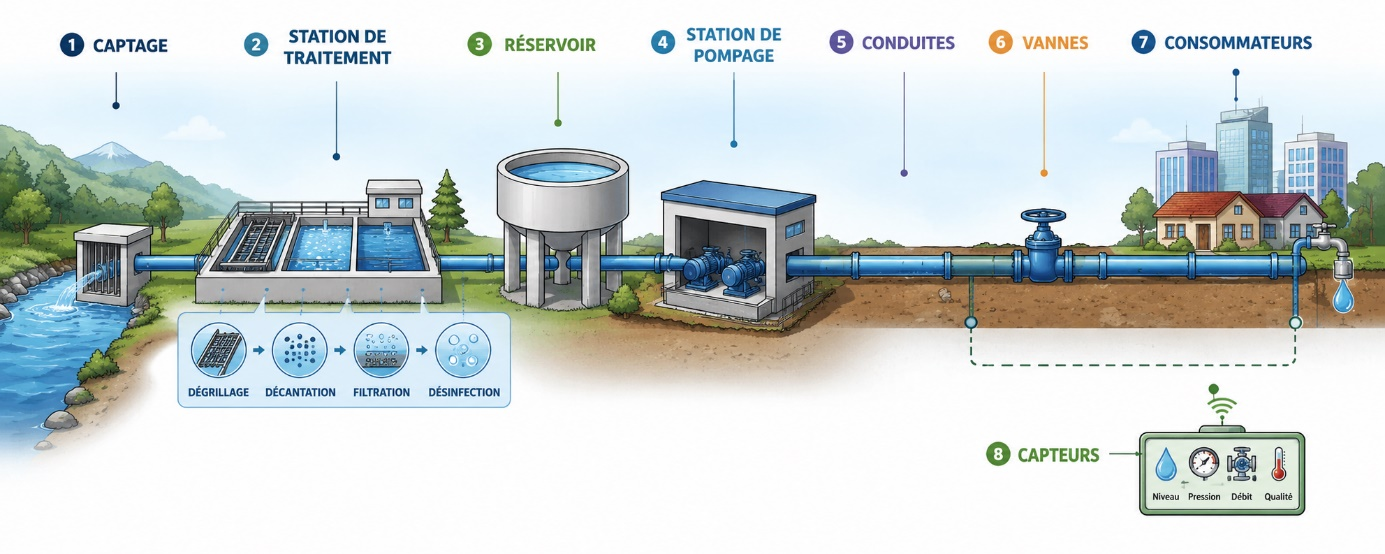
\includegraphics[width=6.3in,height=2.52004in]{figures/image1.jpeg}

Figure 1 Schéma de distribution de l\textquotesingle eau potable

\subsection{1.4. Déploiement d'un réseau de distribution d'eau
potable}\label{duxe9ploiement-dun-ruxe9seau-de-distribution-deau-potable}

Le déploiement d\textquotesingle un réseau de distribution
d\textquotesingle eau potable désigne l\textquotesingle ensemble des
activités techniques, organisationnelles et opérationnelles nécessaires
à la planification, à la conception, à la construction et à
l\textquotesingle extension des infrastructures permettant
d\textquotesingle assurer l\textquotesingle approvisionnement en eau
d\textquotesingle une population donnée. Il s\textquotesingle agit
d\textquotesingle un processus complexe qui doit tenir compte à la fois
des caractéristiques démographiques, géographiques, topographiques et
socio-économiques de la zone concernée. La conception
d\textquotesingle un réseau ne consiste donc pas uniquement à installer
des conduites et des équipements hydrauliques, mais nécessite une
analyse globale des besoins actuels et futurs de la population, de la
disponibilité de la ressource, des contraintes du terrain ainsi que des
capacités techniques et financières disponibles. Une planification
appropriée permet ainsi de concevoir un système capable de répondre
durablement à la demande en eau tout en garantissant un niveau de
service acceptable pour les usagers \cite{ref38}.

La première étape du déploiement d\textquotesingle un réseau consiste
généralement à réaliser une \textbf{analyse des besoins en eau}. Cette
analyse permet d\textquotesingle estimer la quantité
d\textquotesingle eau nécessaire à la population actuelle et
d\textquotesingle anticiper l\textquotesingle évolution future de la
demande. Elle prend notamment en considération le nombre
d\textquotesingle habitants, la consommation domestique, les besoins des
activités commerciales et industrielles, les établissements publics
ainsi que les éventuelles pertes du réseau. Dans les zones urbaines
caractérisées par une croissance démographique importante, les
prévisions doivent également intégrer l\textquotesingle extension
progressive des quartiers et l\textquotesingle apparition de nouvelles
zones d\textquotesingle habitation. Une estimation insuffisante des
besoins peut conduire à un sous-dimensionnement des infrastructures,
tandis qu\textquotesingle une surestimation excessive peut entraîner des
investissements disproportionnés et une sous-utilisation des
équipements. Le dimensionnement du réseau doit donc rechercher un
équilibre entre les besoins à satisfaire, les capacités disponibles et
les perspectives d\textquotesingle évolution de la population \cite{ref39}.

La \textbf{planification spatiale} constitue également une dimension
essentielle du déploiement d\textquotesingle un réseau
d\textquotesingle eau potable. Elle consiste à déterminer la
localisation optimale des conduites, des réservoirs, des stations de
pompage, des vannes et des autres ouvrages hydrauliques en fonction de
la configuration géographique de la zone à desservir. Les systèmes
d\textquotesingle information géographique (SIG) jouent
aujourd\textquotesingle hui un rôle important dans cette démarche, car
ils permettent de représenter spatialement les infrastructures
existantes, d\textquotesingle analyser la topographie,
d\textquotesingle identifier les zones insuffisamment desservies et de
simuler différents scénarios d\textquotesingle extension du réseau.
L\textquotesingle intégration des données géographiques avec les
informations hydrauliques offre ainsi aux gestionnaires une meilleure
compréhension de la distribution spatiale des infrastructures et
facilite la planification des nouveaux investissements \cite{ref40}.

Le \textbf{dimensionnement hydraulique} représente une autre étape
fondamentale du processus de déploiement. Il consiste notamment à
déterminer les diamètres appropriés des conduites, les capacités des
réservoirs, les caractéristiques des pompes et les dispositifs
nécessaires au contrôle de la pression. Les calculs hydrauliques doivent
garantir que l\textquotesingle eau puisse atteindre les différents
points de consommation avec un débit suffisant et une pression
compatible avec les exigences du service. Une pression trop faible peut
empêcher l\textquotesingle alimentation correcte de certaines zones,
tandis qu\textquotesingle une pression excessive peut accélérer la
dégradation des conduites et favoriser l\textquotesingle apparition de
fuites. Des logiciels de simulation hydraulique tels
qu\textquotesingle{}\textbf{EPANET} permettent de modéliser le
comportement d\textquotesingle un réseau et d\textquotesingle analyser
différents scénarios de fonctionnement avant la réalisation effective
des infrastructures. Ces outils constituent ainsi une aide importante à
la conception et à l\textquotesingle optimisation des réseaux de
distribution d\textquotesingle eau potable \cite{ref34}.

Le déploiement d\textquotesingle un réseau doit également prendre en
compte la \textbf{maintenance future des infrastructures}. Un réseau
correctement conçu doit permettre l\textquotesingle accès aux différents
équipements afin de faciliter les opérations
d\textquotesingle inspection, de réparation et de remplacement. La
localisation des vannes doit notamment permettre
d\textquotesingle isoler rapidement les sections défectueuses sans
interrompre l\textquotesingle alimentation de l\textquotesingle ensemble
des usagers. De même, les équipements critiques tels que les pompes et
les réservoirs doivent être intégrés dans une stratégie de maintenance
permettant de réduire les risques de panne et les interruptions de
service. Cette approche implique de ne plus considérer le déploiement
comme une opération ponctuelle, mais comme un processus qui doit
intégrer l\textquotesingle ensemble du cycle de vie des infrastructures,
depuis leur conception jusqu\textquotesingle à leur renouvellement
\cite{ref42}.

Dans les contextes urbains en expansion rapide, le déploiement des
réseaux de distribution d\textquotesingle eau potable présente des
difficultés particulières. L\textquotesingle extension non planifiée des
quartiers, l\textquotesingle occupation progressive des zones
périphériques et l\textquotesingle insuffisance des données actualisées
sur les infrastructures existantes peuvent compliquer considérablement
la planification des nouveaux ouvrages. À cela
s\textquotesingle ajoutent les contraintes liées à la topographie, à la
disponibilité des ressources financières et à la nécessité de maintenir
le service pendant les travaux d\textquotesingle extension. Dans une
ville comme Bukavu, caractérisée par une urbanisation rapide et une
topographie particulièrement accidentée, la planification spatiale et
hydraulique du réseau représente donc un enjeu majeur. La prise en
compte simultanée des données géographiques, des paramètres hydrauliques
et des besoins des populations peut contribuer à améliorer les décisions
relatives à l\textquotesingle extension du réseau vers les zones
insuffisamment desservies \cite{ref43}.

Dans cette perspective, les technologies numériques offrent de nouvelles
possibilités pour améliorer le processus de déploiement des
infrastructures hydrauliques. L\textquotesingle utilisation combinée des
systèmes d\textquotesingle information géographique, de la modélisation
hydraulique, des données issues des capteurs et des techniques
d\textquotesingle intelligence artificielle permet
d\textquotesingle envisager une planification plus dynamique et plus
précise. Un \textbf{jumeau numérique} du réseau pourrait notamment
permettre de représenter virtuellement l\textquotesingle infrastructure
existante et de simuler différents scénarios d\textquotesingle extension
avant leur mise en œuvre réelle. Les gestionnaires pourraient ainsi
évaluer les conséquences d\textquotesingle une nouvelle conduite,
d\textquotesingle un nouveau réservoir ou d\textquotesingle une station
de pompage supplémentaire sur le fonctionnement global du réseau. Cette
capacité de simulation et d\textquotesingle analyse prospective
constitue l\textquotesingle un des intérêts majeurs du jumeau numérique
dans le contexte de la gestion des infrastructures hydrauliques et sera
approfondie dans les sections consacrées aux technologies numériques et
au Digital Twin \cite{ref17}.

\subsection{1.5. Surveillance d'un réseau de distribution d'eau
potable}\label{surveillance-dun-ruxe9seau-de-distribution-deau-potable}

La surveillance d'un réseau de distribution d'eau potable constitue une
activité essentielle pour garantir la continuité, la fiabilité et la
sécurité du service d'approvisionnement en eau. Elle consiste à observer
de manière régulière ou continue l'état des différents composants du
réseau ainsi que l'évolution des principaux paramètres hydrauliques et
physico-chimiques. Parmi les paramètres généralement suivis figurent
notamment la pression, le débit, le niveau des réservoirs, la qualité de
l'eau, la consommation ainsi que l'état de fonctionnement des
équipements tels que les pompes et les vannes.
L\textquotesingle objectif principal de cette surveillance est de
permettre aux gestionnaires d\textquotesingle identifier rapidement
toute situation anormale susceptible d\textquotesingle affecter le
fonctionnement du réseau et la qualité du service fourni aux
consommateurs. Une surveillance efficace contribue ainsi à limiter les
interruptions de distribution, à réduire les pertes
d\textquotesingle eau et à améliorer la capacité des équipes techniques
à intervenir rapidement en cas de problème \cite{ref11}.

Dans les approches traditionnelles, la surveillance des réseaux de
distribution repose principalement sur des inspections réalisées sur le
terrain, des relevés manuels et l\textquotesingle analyse périodique des
données disponibles. Les techniciens peuvent notamment effectuer des
mesures de pression ou de débit à certains points du réseau, inspecter
visuellement les conduites et les équipements accessibles et rechercher
les signes visibles de fuite ou de détérioration. Bien que ces méthodes
restent utiles, elles présentent plusieurs limites, notamment lorsque le
réseau est vaste, complexe ou difficile d\textquotesingle accès. Les
inspections périodiques ne permettent pas nécessairement de détecter
immédiatement une anomalie qui survient entre deux campagnes de
contrôle. De plus, certaines fuites peuvent rester invisibles pendant
une longue période lorsqu\textquotesingle elles se produisent sous terre
ou dans des zones difficilement accessibles. Cette situation peut
entraîner des pertes importantes avant que les équipes techniques ne
soient informées du problème \cite{ref45}.

La surveillance d\textquotesingle un réseau hydraulique doit également
permettre de suivre l\textquotesingle évolution de la \textbf{pression}
et du \textbf{débit}, deux paramètres particulièrement importants pour
évaluer son comportement. Une variation inhabituelle de la pression peut
être associée à différents phénomènes, notamment une rupture de
conduite, une fuite, une obstruction, une mauvaise régulation ou une
modification importante de la demande. De même, une variation anormale
du débit peut révéler une consommation inhabituelle ou signaler une
perte d\textquotesingle eau dans une partie du réseau.
L\textquotesingle analyse simultanée de ces paramètres permet donc
d\textquotesingle obtenir une meilleure compréhension de
l\textquotesingle état hydraulique du système et
d\textquotesingle identifier plus rapidement les situations nécessitant
une intervention. Dans cette perspective, la surveillance ne doit pas se
limiter à la collecte de données, mais doit également permettre leur
interprétation afin de produire des informations utiles à la prise de
décision \cite{ref34}.

Avec l\textquotesingle évolution des technologies numériques, les
réseaux de distribution d\textquotesingle eau peuvent désormais être
équipés de \textbf{capteurs intelligents} capables de mesurer
automatiquement différents paramètres et de transmettre les données vers
une plateforme centrale. Ces dispositifs permettent
d\textquotesingle améliorer considérablement la fréquence et la
précision de la surveillance, tout en réduisant la dépendance aux
interventions manuelles. Les données collectées peuvent être transmises
à intervalles réguliers ou en quasi-temps réel grâce à différentes
technologies de communication. Une plateforme de supervision peut alors
centraliser ces informations et présenter l\textquotesingle état du
réseau sous forme de tableaux de bord, de graphiques et de cartes
interactives. Cette approche permet aux gestionnaires de disposer
d\textquotesingle une vision plus complète de l\textquotesingle état du
système et de réagir plus rapidement lorsqu\textquotesingle une anomalie
est détectée \cite{ref20}.

La surveillance moderne des réseaux d\textquotesingle eau
s\textquotesingle appuie également sur les \textbf{systèmes
d\textquotesingle information géographique (SIG)}, qui permettent de
représenter spatialement les différents composants de
l\textquotesingle infrastructure. Les conduites, les réservoirs, les
stations de pompage, les vannes et les capteurs peuvent ainsi être
localisés sur une carte numérique et associés à des informations
techniques et opérationnelles. Cette représentation géographique
facilite l\textquotesingle identification de la zone concernée
lorsqu\textquotesingle une anomalie est détectée et permet aux équipes
techniques de mieux planifier leurs interventions.
L\textquotesingle intégration des données géographiques avec les données
hydrauliques constitue donc une approche particulièrement intéressante
pour les réseaux urbains complexes, car elle permet de combiner la
dimension spatiale et la dimension opérationnelle du système \cite{ref46}.

Une évolution importante de la surveillance des réseaux
d\textquotesingle eau réside dans le passage d\textquotesingle une
approche \textbf{réactive} à une approche \textbf{proactive et
prédictive}. Dans une approche réactive, l\textquotesingle intervention
est généralement déclenchée après l\textquotesingle apparition
d\textquotesingle une défaillance ou d\textquotesingle une interruption
de service. À l\textquotesingle inverse, une approche proactive cherche
à détecter les premiers signes d\textquotesingle une anomalie afin
d\textquotesingle intervenir avant que celle-ci ne provoque une panne
importante. L\textquotesingle approche prédictive va encore plus loin en
utilisant les données historiques et les techniques
d\textquotesingle analyse avancée pour estimer la probabilité
qu\textquotesingle une défaillance survienne dans le futur. Cette
évolution est rendue possible par la combinaison des capteurs
intelligents, des systèmes de collecte de données, de
l\textquotesingle analyse statistique et de
l\textquotesingle intelligence artificielle. Elle permet potentiellement
de réduire les temps d\textquotesingle intervention,
d\textquotesingle améliorer la maintenance et de limiter les
conséquences des défaillances sur les usagers \cite{ref47}.

Dans le contexte de la présente étude, la surveillance constitue
l\textquotesingle un des éléments centraux du \textbf{jumeau numérique
du réseau de fourniture d\textquotesingle eau potable de la commune de
Kadutu}. Le système envisagé devra permettre de représenter les
principaux composants du réseau sur une plateforme numérique et
d\textquotesingle associer à ces composants des données relatives à leur
état de fonctionnement. Les données issues des capteurs,
qu\textquotesingle elles soient réelles ou simulées dans le cadre du
prototype, pourront être exploitées pour suivre
l\textquotesingle évolution de la pression, du débit et
d\textquotesingle autres paramètres pertinents.
L\textquotesingle intégration d\textquotesingle algorithmes
d\textquotesingle intelligence artificielle permettra ensuite
d\textquotesingle aller au-delà de la simple visualisation des données
en identifiant automatiquement des comportements anormaux et en
fournissant des informations utiles à la maintenance. Ainsi, la
surveillance intelligente constitue une étape fondamentale vers la mise
en place d\textquotesingle un système capable de reproduire
virtuellement l\textquotesingle état du réseau réel et
d\textquotesingle assister les gestionnaires dans leurs décisions
opérationnelles \cite{ref17}.

\subsection{1.6. Maintenance d'un réseau de distribution d'eau
potable}\label{maintenance-dun-ruxe9seau-de-distribution-deau-potable}

La maintenance d'un réseau de distribution d'eau potable regroupe
l'ensemble des actions techniques et organisationnelles visant à
maintenir ou à rétablir les infrastructures hydrauliques dans un état de
fonctionnement permettant d'assurer la continuité, la fiabilité et la
qualité du service. Elle concerne l'ensemble des composants du réseau,
notamment les conduites, les vannes, les stations de pompage, les
réservoirs, les équipements de mesure et les dispositifs de contrôle.
Une stratégie de maintenance efficace permet de prolonger la durée de
vie des infrastructures, de réduire les interruptions de service, de
limiter les pertes d'eau et de maîtriser les coûts
d\textquotesingle exploitation. Dans un contexte où les réseaux sont
soumis au vieillissement, à l\textquotesingle augmentation de la demande
et à différentes contraintes environnementales, la maintenance constitue
donc une fonction essentielle de la gestion durable des systèmes
d\textquotesingle approvisionnement en eau potable \cite{ref42}.

Traditionnellement, la maintenance des réseaux de distribution
d\textquotesingle eau repose sur plusieurs approches complémentaires. La
\textbf{maintenance corrective} intervient après
l\textquotesingle apparition d\textquotesingle une défaillance et
consiste à réparer ou à remplacer l\textquotesingle équipement concerné
afin de rétablir le fonctionnement normal du système. Cette approche est
particulièrement fréquente lorsque les gestionnaires disposent de moyens
limités ou lorsque les infrastructures ne sont pas suffisamment
instrumentées. Toutefois, une maintenance exclusivement corrective
présente des inconvénients importants, car elle implique généralement
une intervention après que le problème s\textquotesingle est déjà
produit. Une rupture de conduite peut, par exemple, provoquer une
interruption de l\textquotesingle approvisionnement, des pertes
importantes d\textquotesingle eau et des dommages aux infrastructures
environnantes avant même que les équipes techniques puissent intervenir.
Cette situation peut également augmenter les coûts de réparation et
perturber considérablement le service fourni aux consommateurs \cite{ref45}.

La \textbf{maintenance préventive}, quant à elle, consiste à réaliser
des opérations d\textquotesingle inspection, de contrôle et
d\textquotesingle entretien selon un calendrier défini à
l\textquotesingle avance, indépendamment de l\textquotesingle apparition
effective d\textquotesingle une panne. Elle peut comprendre le contrôle
périodique des équipements de pompage, l\textquotesingle inspection des
conduites, la vérification des vannes ou encore
l\textquotesingle entretien des réservoirs. L\textquotesingle objectif
est de réduire la probabilité de défaillance et
d\textquotesingle identifier suffisamment tôt les signes de
détérioration. Cette approche présente l\textquotesingle avantage de
permettre une meilleure organisation des interventions et une
planification plus efficace des ressources humaines et matérielles.
Cependant, lorsqu\textquotesingle elle repose uniquement sur des
calendriers fixes, elle ne tient pas nécessairement compte de
l\textquotesingle état réel des équipements ni de leur évolution dans le
temps. Certaines infrastructures peuvent ainsi être entretenues alors
qu\textquotesingle elles ne présentent aucun signe de dégradation,
tandis que d\textquotesingle autres peuvent développer des anomalies
entre deux périodes d\textquotesingle inspection \cite{ref49}.

Une approche plus avancée est la \textbf{maintenance prédictive}, qui
consiste à utiliser les données provenant des équipements et des
systèmes de surveillance afin d\textquotesingle anticiper les
défaillances potentielles. Contrairement à la maintenance corrective et
à la maintenance préventive classique, cette approche
s\textquotesingle appuie sur l\textquotesingle analyse de
l\textquotesingle état réel du système. Les données relatives à la
pression, au débit, aux vibrations, à la consommation énergétique, à
l\textquotesingle âge des équipements ou encore à
l\textquotesingle historique des interventions peuvent être analysées
afin d\textquotesingle identifier des tendances annonciatrices
d\textquotesingle une défaillance. L\textquotesingle objectif est de
permettre aux gestionnaires d\textquotesingle intervenir au moment le
plus approprié, avant qu\textquotesingle une panne importante ne
survienne, tout en évitant les opérations d\textquotesingle entretien
inutiles. La maintenance prédictive peut ainsi contribuer à améliorer la
disponibilité des infrastructures et à optimiser
l\textquotesingle utilisation des ressources consacrées à leur entretien
\cite{ref47}.

Dans les réseaux de distribution d\textquotesingle eau potable, les
\textbf{fuites} représentent l\textquotesingle un des problèmes majeurs
auxquels les stratégies de maintenance doivent répondre. Une fuite peut
résulter du vieillissement des conduites, de la corrosion, de mouvements
du sol, d\textquotesingle une pression excessive ou encore de défauts au
niveau des raccordements. Certaines fuites sont facilement visibles et
peuvent être détectées rapidement, tandis que d\textquotesingle autres
restent souterraines et peuvent persister pendant de longues périodes.
Ces fuites dites invisibles peuvent provoquer des pertes importantes
d\textquotesingle eau et contribuer à l\textquotesingle augmentation de
l\textquotesingle{}\textbf{eau non facturée} (\emph{Non-Revenue Water --
NRW}). La détection précoce des fuites constitue donc un objectif
essentiel de la maintenance moderne des réseaux hydrauliques. Elle
nécessite l\textquotesingle utilisation combinée de méthodes
traditionnelles d\textquotesingle inspection et de technologies avancées
de surveillance et d\textquotesingle analyse des données \cite{ref50}.

L\textquotesingle intégration des \textbf{capteurs intelligents}
constitue à cet égard une évolution importante des stratégies de
maintenance. En mesurant en continu ou à intervalles réguliers les
paramètres caractéristiques du réseau, les capteurs permettent de
disposer d\textquotesingle informations actualisées sur
l\textquotesingle état des infrastructures. Une variation inhabituelle
de pression peut, par exemple, signaler une fuite ou une rupture
potentielle, tandis qu\textquotesingle une modification du débit peut
indiquer une consommation anormale ou une perte d\textquotesingle eau.
Ces informations peuvent être transmises à une plateforme centrale afin
d\textquotesingle être analysées automatiquement. La maintenance peut
alors être déclenchée sur la base de données objectives relatives à
l\textquotesingle état réel du réseau plutôt que sur la seule base
d\textquotesingle un calendrier fixe ou d\textquotesingle une
intervention après panne \cite{ref20}.

L\textquotesingle intelligence artificielle offre également des
possibilités nouvelles dans le domaine de la maintenance des réseaux
d\textquotesingle eau potable. Les algorithmes
d\textquotesingle apprentissage automatique peuvent être entraînés à
partir de données historiques afin d\textquotesingle identifier des
relations complexes entre les paramètres hydrauliques et
l\textquotesingle apparition de défaillances. Des modèles peuvent ainsi
être utilisés pour détecter des anomalies, estimer la probabilité de
rupture d\textquotesingle une conduite ou prévoir
l\textquotesingle évolution de certains indicateurs de performance.
L\textquotesingle efficacité de ces approches dépend toutefois de la
qualité et de la quantité des données disponibles, ainsi que de la
capacité du modèle à représenter correctement les caractéristiques du
réseau étudié. L\textquotesingle intelligence artificielle doit donc
être considérée comme un outil d\textquotesingle aide à la décision
venant compléter l\textquotesingle expertise des gestionnaires et non
comme un remplacement systématique de l\textquotesingle intervention
humaine \cite{ref51}.

Dans le cadre du présent travail, la maintenance constitue une dimension
fondamentale du \textbf{jumeau numérique intégrant
l\textquotesingle intelligence artificielle}. Le système proposé doit
permettre de représenter l\textquotesingle état des principales
infrastructures du réseau de la commune de Kadutu et
d\textquotesingle exploiter les données disponibles afin
d\textquotesingle identifier les situations susceptibles de nécessiter
une intervention. L\textquotesingle intégration de mécanismes de
détection d\textquotesingle anomalies et d\textquotesingle analyse
prédictive pourrait ainsi contribuer à passer progressivement
d\textquotesingle une logique essentiellement corrective à une logique
plus proactive et prédictive. La plateforme numérique envisagée pourrait
notamment signaler une baisse anormale de pression, détecter une
situation susceptible de correspondre à une fuite et fournir aux
gestionnaires des informations facilitant la priorisation des
interventions. Cette approche permettrait d\textquotesingle améliorer la
réactivité des équipes techniques et de contribuer à une gestion plus
efficace des infrastructures hydrauliques.

Ainsi, la maintenance et la surveillance sont étroitement liées. La
surveillance fournit les données nécessaires à la connaissance de
l\textquotesingle état du réseau, tandis que la maintenance transforme
ces informations en actions concrètes destinées à préserver ou à
rétablir les performances du système. Dans une architecture fondée sur
le jumeau numérique, ces deux fonctions peuvent être réunies au sein
d\textquotesingle un environnement numérique capable de recevoir des
données provenant du réseau réel, de les analyser, de représenter
l\textquotesingle état actuel du système et de simuler son évolution
future. Cette intégration ouvre la voie à une gestion plus intelligente
et plus anticipative des infrastructures d\textquotesingle eau potable,
ce qui constitue une transition naturelle vers l\textquotesingle étude
des \textbf{technologies numériques appliquées à la gestion des réseaux
hydrauliques}.

\subsection{1.7. Technologies numériques appliquées à la gestion des
réseaux d\textquotesingle eau
potable}\label{technologies-numuxe9riques-appliquuxe9es-uxe0-la-gestion-des-ruxe9seaux-deau-potable}

La transformation numérique des infrastructures hydrauliques constitue
aujourd\textquotesingle hui une évolution importante dans le domaine de
la gestion des réseaux d\textquotesingle eau potable. Pendant longtemps,
la gestion de ces infrastructures a reposé principalement sur des
méthodes traditionnelles caractérisées par des relevés manuels, des
inspections périodiques et des interventions techniques déclenchées
après l\textquotesingle apparition de défaillances. Toutefois,
l\textquotesingle augmentation de la demande en eau, le vieillissement
des infrastructures, les contraintes financières et la nécessité de
réduire les pertes d\textquotesingle eau imposent progressivement aux
gestionnaires d\textquotesingle adopter de nouvelles méthodes de
surveillance et de prise de décision. Dans ce contexte, les technologies
numériques offrent la possibilité de transformer les réseaux
traditionnels en systèmes plus intelligents, capables de collecter, de
transmettre, d\textquotesingle analyser et d\textquotesingle exploiter
de grandes quantités de données afin d\textquotesingle améliorer leur
fonctionnement. Cette transformation repose notamment sur la combinaison
des systèmes d\textquotesingle information géographique, de
l\textquotesingle Internet des objets, des capteurs intelligents, du Big
Data, de l\textquotesingle informatique en nuage, des systèmes de
supervision et de l\textquotesingle intelligence artificielle \cite{ref42}.

L\textquotesingle un des premiers outils numériques largement utilisés
dans la gestion des infrastructures hydrauliques est le \textbf{Système
d\textquotesingle Information Géographique (SIG)}. Un SIG est un système
informatique permettant de collecter, stocker, organiser, analyser et
représenter des informations associées à une position géographique. Dans
le domaine de l\textquotesingle eau potable, il permet notamment de
cartographier les conduites, les réservoirs, les stations de pompage,
les vannes, les compteurs et les différents équipements du réseau.
Chaque élément peut être associé à des informations descriptives telles
que son âge, son matériau, son diamètre, son état ou son historique de
maintenance. Cette capacité à associer des données géographiques et
techniques facilite la connaissance du patrimoine hydraulique et
améliore la planification des opérations de maintenance et
d\textquotesingle extension. Dans une ville comme Bukavu, où la
croissance urbaine et les contraintes topographiques peuvent compliquer
la gestion des infrastructures, l\textquotesingle utilisation
d\textquotesingle un SIG peut constituer un outil important pour
visualiser la répartition spatiale du réseau et identifier les zones
insuffisamment desservies \cite{ref52}.

Une autre technologie essentielle est
l\textquotesingle{}\textbf{Internet des objets (Internet of Things --
IoT)}. L\textquotesingle IoT désigne un ensemble de technologies
permettant à des objets physiques équipés de capteurs, de dispositifs
électroniques et de moyens de communication de collecter et
d\textquotesingle échanger automatiquement des données avec
d\textquotesingle autres systèmes. Dans le contexte des réseaux
d\textquotesingle eau potable, cette technologie permet
d\textquotesingle équiper les infrastructures de dispositifs capables de
mesurer différents paramètres tels que la pression, le débit, le niveau
des réservoirs, la qualité de l\textquotesingle eau ou encore les
vibrations des conduites. Les données collectées peuvent ensuite être
transmises vers une plateforme de traitement afin d\textquotesingle être
analysées et exploitées. L\textquotesingle IoT contribue ainsi à
transformer des infrastructures physiques traditionnelles en systèmes
instrumentés capables de fournir en permanence des informations sur leur
état de fonctionnement \cite{ref20}.

Les \textbf{capteurs intelligents} constituent l\textquotesingle un des
principaux éléments permettant la mise en œuvre de l\textquotesingle IoT
dans les réseaux hydrauliques. Contrairement aux dispositifs de mesure
classiques, les capteurs intelligents peuvent intégrer des capacités de
traitement, de communication et parfois de diagnostic. Ils permettent de
collecter automatiquement des données à différents endroits du réseau et
de transmettre ces informations vers un système centralisé. Les capteurs
de pression peuvent notamment contribuer à identifier des variations
anormales susceptibles d\textquotesingle être associées à une fuite ou à
une rupture de conduite. Les capteurs de débit permettent quant à eux de
suivre les volumes d\textquotesingle eau transportés et de détecter des
écarts entre les débits attendus et les débits mesurés.
D\textquotesingle autres dispositifs peuvent être utilisés pour
surveiller le niveau des réservoirs ou certains paramètres liés à la
qualité de l\textquotesingle eau. L\textquotesingle installation de ces
capteurs constitue donc une étape essentielle pour disposer de données
suffisamment précises et actualisées sur l\textquotesingle état du
réseau \cite{ref47}.

La gestion numérique des réseaux d\textquotesingle eau implique
également le traitement d\textquotesingle un volume important de données
provenant de sources multiples. Cette problématique est généralement
associée au concept de \textbf{Big Data}, qui désigne des ensembles de
données caractérisés notamment par leur volume, leur variété, leur
vitesse de génération et leur complexité. Dans un réseau intelligent,
les informations peuvent provenir simultanément des capteurs
hydrauliques, des compteurs, des systèmes géographiques, des historiques
de maintenance et des données météorologiques ou démographiques.
L\textquotesingle analyse de ces données peut permettre
d\textquotesingle identifier des tendances, de détecter des
comportements inhabituels et de mieux comprendre les facteurs
influençant les performances du réseau. Toutefois, la valeur de ces
données dépend fortement de leur qualité, de leur disponibilité et de la
capacité du système à les organiser et à les exploiter efficacement
\cite{ref17}.

L\textquotesingle{}\textbf{informatique en nuage (Cloud Computing)}
constitue également une technologie importante pour la gestion des
données issues des infrastructures hydrauliques. Elle permet de stocker
et de traiter des données sur des infrastructures informatiques
distantes accessibles à travers un réseau. Cette approche peut faciliter
la centralisation des informations provenant de différents équipements
et permettre leur consultation depuis plusieurs points
d\textquotesingle accès. Dans le contexte d\textquotesingle une
plateforme intelligente de gestion de l\textquotesingle eau, les données
collectées par les capteurs peuvent être stockées dans une base de
données centralisée et exploitées par différentes applications. Les
gestionnaires peuvent ainsi accéder aux informations nécessaires à la
surveillance et à la prise de décision sans dépendre
d\textquotesingle un stockage local unique. Le recours au Cloud
Computing doit cependant être accompagné de mesures appropriées
concernant la sécurité des données, la disponibilité des services et la
protection des communications \cite{ref53}.

Les \textbf{systèmes de supervision et d\textquotesingle acquisition de
données}, communément appelés systèmes \textbf{SCADA (Supervisory
Control and Data Acquisition)}, jouent également un rôle important dans
la surveillance des infrastructures hydrauliques. Ces systèmes
permettent de collecter des informations provenant de différents
équipements, de les centraliser et de présenter leur état aux opérateurs
à travers une interface de supervision. Dans les réseaux
d\textquotesingle eau potable, un système SCADA peut notamment être
utilisé pour surveiller les stations de pompage, les niveaux des
réservoirs, les pressions ou certains paramètres de fonctionnement des
équipements. Il peut également permettre aux opérateurs de contrôler
certains dispositifs à distance. Cependant, contrairement au jumeau
numérique, un système SCADA est principalement orienté vers la
supervision et le contrôle du système physique. Le jumeau numérique
ajoute une dimension de représentation virtuelle, de simulation et
d\textquotesingle analyse avancée permettant d\textquotesingle explorer
différents scénarios et d\textquotesingle anticiper les évolutions
futures du système \cite{ref54}.

L\textquotesingle{}\textbf{intelligence artificielle (IA)} constitue une
autre composante majeure de la transformation numérique des réseaux
d\textquotesingle eau. Elle regroupe un ensemble de méthodes permettant
à des systèmes informatiques d\textquotesingle effectuer des tâches
nécessitant généralement certaines capacités d\textquotesingle analyse
et de raisonnement. Dans le domaine de l\textquotesingle eau, les
techniques d\textquotesingle intelligence artificielle peuvent être
utilisées pour détecter des anomalies, prévoir la demande, identifier
les risques de fuite, estimer la probabilité de défaillance des
infrastructures ou optimiser certaines opérations.
L\textquotesingle apprentissage automatique (\emph{Machine Learning})
permet notamment aux modèles informatiques d\textquotesingle identifier
des relations dans les données historiques et de produire des
prédictions à partir de nouvelles observations. Dans le cadre de la
présente étude, l\textquotesingle IA pourra ainsi être utilisée pour
analyser les données hydrauliques et identifier automatiquement des
comportements inhabituels susceptibles d\textquotesingle indiquer une
anomalie dans le réseau \cite{ref55}.

Ces différentes technologies ne doivent cependant pas être considérées
comme des solutions indépendantes. Leur véritable potentiel apparaît
lorsqu\textquotesingle elles sont intégrées au sein
d\textquotesingle une architecture numérique cohérente. Les capteurs
permettent de collecter les données, l\textquotesingle IoT assure leur
communication, les bases de données et le Cloud permettent leur
stockage, les SIG assurent leur représentation spatiale, les systèmes de
supervision permettent leur visualisation et
l\textquotesingle intelligence artificielle contribue à leur analyse
avancée. Cette combinaison forme une chaîne technologique capable de
transformer un réseau physique en une infrastructure intelligente, mieux
observable et plus facilement pilotable. Dans cette architecture, le
\textbf{jumeau numérique} peut jouer le rôle d\textquotesingle une
couche d\textquotesingle intégration permettant de relier la
représentation virtuelle du réseau aux données issues du système
physique et aux modèles d\textquotesingle analyse \cite{ref56}.

Dans le cadre de ce travail, l\textquotesingle utilisation de ces
technologies sera envisagée de manière progressive et adaptée aux
objectifs du projet. Le système proposé reposera notamment sur une
représentation numérique du réseau de fourniture d\textquotesingle eau
potable de la commune de Kadutu, associée à des données provenant de
capteurs réels ou simulés. Ces données pourront être utilisées pour
représenter l\textquotesingle état du réseau, visualiser les variations
de pression et de débit, simuler des anomalies et analyser les
performances du système. L\textquotesingle intelligence artificielle
sera ensuite intégrée afin de renforcer les capacités de détection des
anomalies et d\textquotesingle aide à la décision.
L\textquotesingle objectif final est ainsi de construire une plateforme
numérique capable de fournir une représentation dynamique du réseau et
de faciliter sa surveillance et sa maintenance.

L\textquotesingle ensemble de ces technologies constitue donc le socle
technique sur lequel peut être construit un système de gestion
intelligente des infrastructures hydrauliques. Toutefois, leur
intégration nécessite une architecture capable de maintenir une relation
cohérente entre le système physique, les données collectées et sa
représentation numérique. C\textquotesingle est précisément cette
problématique qui conduit au concept de \textbf{jumeau numérique},
lequel sera étudié plus en profondeur dans la section suivante. Cette
notion constitue le cœur technologique du présent travail,
puisqu\textquotesingle elle permettra d\textquotesingle établir le lien
entre le réseau réel de fourniture d\textquotesingle eau potable, les
données collectées par les capteurs et les modèles
d\textquotesingle intelligence artificielle destinés à améliorer la
surveillance et la maintenance du système.

\subsection{1.8. Le concept de jumeau numérique (Digital
Twin)}\label{le-concept-de-jumeau-numuxe9rique-digital-twin}

Le concept de \textbf{jumeau numérique}, communément désigné par
l\textquotesingle expression anglaise \emph{Digital Twin}, représente
une évolution importante dans le domaine des technologies numériques
appliquées aux systèmes complexes. De manière générale, un jumeau
numérique peut être défini comme une représentation numérique dynamique
d\textquotesingle un objet, d\textquotesingle un processus,
d\textquotesingle une infrastructure ou d\textquotesingle un système
physique réel, maintenue en relation avec celui-ci grâce à un échange
continu ou périodique de données. Contrairement à une simple
représentation numérique statique, le jumeau numérique est conçu pour
évoluer en fonction de l\textquotesingle état et du comportement du
système physique qu\textquotesingle il représente. Il peut ainsi être
utilisé pour observer, analyser, simuler et prédire le comportement
d\textquotesingle un système réel dans différentes situations. Cette
capacité à établir une relation entre un système physique et son
équivalent numérique fait du jumeau numérique une technologie
particulièrement intéressante pour la gestion des infrastructures
complexes nécessitant une surveillance permanente et une prise de
décision fondée sur les données \cite{ref8}.

L\textquotesingle idée fondamentale à l\textquotesingle origine du
jumeau numérique repose sur la création d\textquotesingle un lien étroit
entre le monde physique et le monde numérique. Dans une architecture
classique, les données relatives à une infrastructure sont généralement
collectées et stockées séparément des modèles utilisés pour son analyse.
Le jumeau numérique cherche au contraire à rapprocher ces deux
dimensions en permettant à la représentation virtuelle de recevoir
régulièrement des informations provenant du système réel. Les données
collectées peuvent concerner l\textquotesingle état des équipements, les
conditions de fonctionnement, les performances ou encore
l\textquotesingle environnement dans lequel le système évolue. Grâce à
ces informations, la représentation numérique peut être actualisée afin
de refléter aussi fidèlement que possible la situation du système
physique à un instant donné. Cette relation dynamique constitue
l\textquotesingle une des principales caractéristiques qui distinguent
le jumeau numérique des modèles numériques traditionnels \cite{ref58}.

Le développement du concept de jumeau numérique est généralement associé
aux travaux de \textbf{Michael Grieves}, qui a introduit le concept de
\emph{Virtual Digital Representation} dans le contexte de la gestion du
cycle de vie des produits. Les travaux de Grieves ont contribué à
formaliser l\textquotesingle idée selon laquelle un produit ou un
système physique pouvait être associé à une représentation virtuelle
permettant de conserver et d\textquotesingle exploiter les informations
relatives à son cycle de vie. Par la suite, l\textquotesingle évolution
des technologies de capteurs, de l\textquotesingle Internet des objets,
de l\textquotesingle informatique en nuage, de
l\textquotesingle intelligence artificielle et des capacités de calcul a
progressivement rendu possible la mise en œuvre de jumeaux numériques
plus complexes et plus dynamiques. Le concept s\textquotesingle est
ainsi étendu au-delà du domaine industriel pour être appliqué à de
nombreux secteurs, notamment les transports, l\textquotesingle énergie,
la santé, les bâtiments, les villes intelligentes et les infrastructures
hydrauliques \cite{ref59}.

Il est important de distinguer le \textbf{jumeau numérique}
d\textquotesingle autres concepts proches tels que le modèle numérique,
la simulation numérique ou la maquette numérique. Un modèle numérique
constitue généralement une représentation mathématique ou informatique
d\textquotesingle un système réel utilisée pour analyser certains de ses
comportements. Une simulation permet ensuite d\textquotesingle utiliser
ce modèle afin d\textquotesingle étudier la réaction du système dans
différentes conditions ou différents scénarios. Une maquette numérique,
quant à elle, représente principalement les caractéristiques
géométriques ou structurelles d\textquotesingle un objet ou
d\textquotesingle une infrastructure. Le jumeau numérique intègre ces
différentes dimensions, mais ajoute une caractéristique fondamentale :
la connexion avec le système physique réel à travers un flux de données.
Il ne s\textquotesingle agit donc pas uniquement de représenter ou de
simuler un système, mais de maintenir une représentation virtuelle
capable d\textquotesingle évoluer en fonction des informations provenant
du système réel \cite{ref17}.

Le fonctionnement d\textquotesingle un jumeau numérique repose
généralement sur trois éléments fondamentaux : \textbf{le système
physique réel, le modèle ou système virtuel et le mécanisme
d\textquotesingle échange de données}. Le système physique représente
l\textquotesingle infrastructure ou l\textquotesingle objet réel dont on
souhaite suivre l\textquotesingle état et le comportement. Le système
virtuel constitue sa représentation numérique et peut intégrer des
modèles géométriques, hydrauliques, mathématiques ou comportementaux.
Enfin, le mécanisme d\textquotesingle échange de données assure la
circulation des informations entre les deux environnements. Dans le sens
du physique vers le numérique, les capteurs collectent les données
relatives à l\textquotesingle état réel du système et les transmettent
au jumeau numérique. Dans le sens inverse, les résultats des analyses et
des simulations peuvent être utilisés pour orienter les décisions des
gestionnaires ou, dans certains systèmes automatisés, pour commander
certains équipements physiques. Cette architecture bidirectionnelle
permet de créer une boucle continue entre observation, analyse,
prédiction et action \cite{ref60}.

Dans le domaine des infrastructures hydrauliques, le jumeau numérique
peut être utilisé pour représenter virtuellement un réseau de
distribution d\textquotesingle eau potable. Le système physique comprend
alors les différents éléments du réseau, notamment les conduites, les
réservoirs, les stations de pompage, les vannes et les points de
consommation. La représentation numérique peut intégrer une carte du
réseau, un modèle hydraulique ainsi que les informations relatives à
l\textquotesingle état des équipements. Les données provenant des
capteurs de pression, de débit et de niveau peuvent être utilisées pour
actualiser la représentation virtuelle et suivre
l\textquotesingle évolution du réseau. Le jumeau numérique peut
également intégrer des modèles de simulation permettant
d\textquotesingle étudier les conséquences d\textquotesingle une
variation de la demande, d\textquotesingle une rupture de conduite ou
d\textquotesingle une modification de la pression. Il devient ainsi un
environnement permettant de mieux comprendre le comportement du réseau
et d\textquotesingle évaluer différents scénarios sans intervenir
directement sur l\textquotesingle infrastructure physique \cite{ref20}.

L\textquotesingle un des principaux avantages du jumeau numérique réside
dans sa capacité à faciliter la \textbf{surveillance en temps réel ou
quasi temps réel}. En intégrant les données issues de capteurs, la
plateforme numérique peut fournir aux gestionnaires une représentation
actualisée de l\textquotesingle état du système. Dans le cas
d\textquotesingle un réseau d\textquotesingle eau potable, une variation
anormale de pression ou de débit peut être visualisée sur la plateforme
et associée à une zone géographique précise. Cette capacité de
visualisation facilite l\textquotesingle identification des anomalies et
permet aux équipes techniques de disposer d\textquotesingle une
meilleure connaissance de la situation avant
d\textquotesingle intervenir sur le terrain. Le jumeau numérique peut
ainsi contribuer à réduire le délai entre l\textquotesingle apparition
d\textquotesingle un problème et sa détection, ce qui constitue un
avantage important dans la gestion des infrastructures hydrauliques
\cite{ref17}.

Le jumeau numérique peut également être utilisé pour effectuer des
\textbf{simulations et des analyses prédictives}. Une fois que le
système virtuel est suffisamment représentatif du système physique, les
gestionnaires peuvent l\textquotesingle utiliser pour tester différents
scénarios. Il est par exemple possible de simuler la fermeture
d\textquotesingle une vanne, l\textquotesingle arrêt
d\textquotesingle une pompe, l\textquotesingle apparition
d\textquotesingle une fuite ou l\textquotesingle extension du réseau
vers une nouvelle zone. Ces simulations permettent
d\textquotesingle anticiper les conséquences potentielles
d\textquotesingle une décision avant sa mise en œuvre réelle.
L\textquotesingle intégration de techniques
d\textquotesingle intelligence artificielle permet en outre
d\textquotesingle analyser les données historiques et actuelles afin
d\textquotesingle identifier des tendances et de produire des
prédictions. Le jumeau numérique devient alors un outil
d\textquotesingle aide à la décision capable de soutenir les
gestionnaires dans la planification de la maintenance et dans
l\textquotesingle optimisation du fonctionnement du réseau \cite{ref61}.

Dans le cadre de la présente étude, le jumeau numérique est envisagé
comme une \textbf{représentation virtuelle dynamique du réseau de
fourniture d\textquotesingle eau potable de la commune de Kadutu}. Il
devra intégrer les principaux composants du système hydraulique,
notamment les conduites, les réservoirs, les stations de pompage, les
vannes et les points de consommation. La plateforme devra également
permettre de représenter les données provenant des capteurs,
qu\textquotesingle elles soient issues de dispositifs réels ou de
données simulées dans le cadre du prototype développé.
L\textquotesingle objectif est de créer un environnement numérique
permettant de visualiser l\textquotesingle état du réseau, de suivre
l\textquotesingle évolution des paramètres hydrauliques, de simuler
certaines anomalies et d\textquotesingle exploiter les capacités de
l\textquotesingle intelligence artificielle pour améliorer la détection
des problèmes et l\textquotesingle aide à la décision.

Ainsi, le jumeau numérique apparaît comme une technologie
particulièrement adaptée aux problématiques de surveillance et de
maintenance des réseaux d\textquotesingle eau potable. Toutefois, sa
mise en œuvre efficace nécessite l\textquotesingle intégration de
plusieurs technologies complémentaires, notamment les capteurs
intelligents, l\textquotesingle Internet des objets, les systèmes
d\textquotesingle information géographique, les modèles hydrauliques,
les bases de données et l\textquotesingle intelligence artificielle. La
qualité du jumeau numérique dépend également de la qualité des données
utilisées pour alimenter et actualiser sa représentation virtuelle. Dans
le cadre de ce travail, cette architecture sera adaptée aux contraintes
du contexte étudié afin de proposer une solution techniquement
réalisable et capable de démontrer le potentiel de cette approche pour
la gestion du réseau de la commune de Kadutu.

\subsection{\texorpdfstring{\textbf{1.9. Architecture et fonctionnement
d\textquotesingle un jumeau
numérique}}{1.9. Architecture et fonctionnement d\textquotesingle un jumeau numérique}}\label{architecture-et-fonctionnement-dun-jumeau-numuxe9rique}

L\textquotesingle efficacité d\textquotesingle un jumeau numérique
repose principalement sur son architecture, c\textquotesingle est-à-dire
sur l\textquotesingle organisation des différents composants matériels
et logiciels qui assurent la communication entre le système physique et
sa représentation virtuelle. Contrairement à une simple simulation
informatique réalisée de manière ponctuelle, un jumeau numérique
fonctionne comme un écosystème numérique intégré dans lequel les données
circulent continuellement entre les équipements physiques, les systèmes
de communication, les bases de données, les modèles numériques et les
outils d\textquotesingle analyse. Cette architecture permet non
seulement de représenter l\textquotesingle état actuel du système, mais
également d\textquotesingle analyser son comportement, de prévoir son
évolution et de proposer des actions permettant
d\textquotesingle améliorer son fonctionnement. La qualité des décisions
produites par un jumeau numérique dépend donc directement de la qualité
de son architecture ainsi que de l\textquotesingle intégration
harmonieuse de ses différentes composantes \cite{ref60}.

De manière générale, l\textquotesingle architecture d\textquotesingle un
jumeau numérique peut être représentée sous la forme de plusieurs
couches fonctionnelles interconnectées. La première couche correspond au
\textbf{système physique}, c\textquotesingle est-à-dire
l\textquotesingle ensemble des infrastructures réelles que le jumeau
numérique est chargé de représenter. Dans le cadre d\textquotesingle un
réseau de distribution d\textquotesingle eau potable, cette couche
comprend notamment les ouvrages de captage, les stations de traitement,
les réservoirs, les stations de pompage, les conduites, les vannes, les
compteurs, les capteurs ainsi que les différents points de consommation.
Ces infrastructures constituent la source principale des données
utilisées pour alimenter le modèle numérique. Leur état évolue
continuellement sous l\textquotesingle effet des conditions
d\textquotesingle exploitation, des variations de consommation et des
interventions de maintenance. Il est donc indispensable que le jumeau
numérique puisse disposer d\textquotesingle informations suffisamment
représentatives de cette réalité physique afin d\textquotesingle assurer
une représentation fidèle du système étudié \cite{ref8}.

La deuxième couche est constituée des \textbf{capteurs intelligents} et
des dispositifs d\textquotesingle acquisition des données. Ces
équipements assurent la collecte des informations relatives au
fonctionnement du système physique. Selon les besoins de
l\textquotesingle application, différents types de capteurs peuvent être
installés afin de mesurer la pression, le débit, le niveau des
réservoirs, la qualité de l\textquotesingle eau, la consommation ou
encore l\textquotesingle état de certains équipements. Les données
collectées sont ensuite converties en informations numériques
exploitables par les autres composantes du système. Dans les
architectures modernes, cette collecte peut être réalisée de manière
continue ou à intervalles réguliers afin de disposer
d\textquotesingle informations actualisées sur l\textquotesingle état du
réseau. Dans le cadre du présent travail, ces données pourront provenir
soit de capteurs réels lorsqu\textquotesingle ils sont disponibles, soit
de données simulées permettant de reproduire le comportement attendu du
réseau dans un environnement expérimental \cite{ref20}.

Une fois collectées, les données doivent être transmises vers une
plateforme de traitement grâce à une \textbf{couche de communication}.
Cette couche assure la circulation des informations entre les
équipements physiques et les applications numériques. Plusieurs
technologies peuvent être utilisées à cette fin, notamment les réseaux
Ethernet, le Wi-Fi, les réseaux cellulaires (4G ou 5G), les protocoles
MQTT, LoRaWAN ou encore NB-IoT, selon les contraintes techniques,
économiques et géographiques du système étudié. La fiabilité de cette
communication est essentielle, car toute interruption ou perte
importante de données peut affecter la qualité de la représentation
numérique. Dans les infrastructures critiques telles que les réseaux
d\textquotesingle eau potable, cette couche doit également intégrer des
mécanismes garantissant la sécurité des communications, la
confidentialité des données et la disponibilité du service \cite{ref62}.

Les données transmises sont ensuite enregistrées dans une \textbf{base
de données}, qui constitue la mémoire du jumeau numérique. Cette base de
données permet de conserver les informations historiques et les données
les plus récentes provenant du réseau. Elle facilite
l\textquotesingle organisation des informations, leur consultation, leur
mise à jour et leur exploitation par les différents modules du système.
Les bases de données relationnelles telles que PostgreSQL ou MySQL,
ainsi que les bases de données NoSQL comme Firebase Firestore ou
MongoDB, sont aujourd\textquotesingle hui largement utilisées dans les
applications de surveillance des infrastructures. Le choix de la
solution dépend généralement du volume des données, de leur fréquence de
mise à jour et des exigences de performance de la plateforme. Une bonne
organisation des données constitue une condition essentielle pour
garantir l\textquotesingle efficacité des analyses réalisées par le
jumeau numérique \cite{ref63}.

Au cœur de l\textquotesingle architecture se trouve le \textbf{modèle
numérique}, qui représente virtuellement le système physique. Ce modèle
constitue l\textquotesingle élément central du jumeau numérique
puisqu\textquotesingle il reproduit la structure, les caractéristiques
et le comportement du réseau réel. Dans le cas d\textquotesingle un
réseau de distribution d\textquotesingle eau potable, il peut intégrer
la cartographie des infrastructures, les caractéristiques hydrauliques
des conduites, les propriétés des équipements ainsi que les relations
existantes entre les différents composants. Ce modèle est
continuellement mis à jour grâce aux données provenant des capteurs afin
de refléter le plus fidèlement possible l\textquotesingle état réel du
réseau. Contrairement à une simple maquette numérique statique, le
modèle numérique d\textquotesingle un jumeau est évolutif et capable de
représenter les changements observés dans le système physique \cite{ref58}.

L\textquotesingle{}\textbf{intelligence artificielle} constitue une
couche complémentaire particulièrement importante dans les architectures
modernes de jumeaux numériques. Les données stockées dans la base
peuvent être analysées à l\textquotesingle aide de différentes
techniques d\textquotesingle apprentissage automatique afin
d\textquotesingle identifier des comportements inhabituels, de détecter
des anomalies ou de produire des prédictions concernant
l\textquotesingle évolution future du système. Plusieurs approches
peuvent être utilisées selon les objectifs poursuivis, notamment les
arbres de décision, les forêts aléatoires (\emph{Random Forest}), les
réseaux de neurones artificiels, les méthodes de détection
d\textquotesingle anomalies ou encore les modèles de séries temporelles.
Dans le cadre de cette étude, l\textquotesingle intelligence
artificielle sera principalement utilisée pour analyser les variations
des paramètres hydrauliques, détecter des situations anormales et
assister les gestionnaires dans la planification des opérations de
maintenance. Cette couche transforme ainsi les données brutes en
informations directement exploitables pour la prise de décision
\cite{ref61}.

Les résultats des analyses sont ensuite présentés aux utilisateurs à
travers une \textbf{interface de visualisation}. Cette interface
constitue le point de contact entre le jumeau numérique et les
gestionnaires du réseau. Elle permet de représenter graphiquement les
infrastructures, de visualiser les paramètres hydrauliques en temps
réel, de consulter les alertes générées par le système et
d\textquotesingle analyser différents indicateurs de performance. Les
tableaux de bord interactifs, les cartes dynamiques, les graphiques
d\textquotesingle évolution, les jauges de pression ou encore les
modèles tridimensionnels facilitent la compréhension du comportement du
réseau et améliorent la qualité des décisions prises par les opérateurs.
Une interface ergonomique et intuitive constitue donc un élément
essentiel de la réussite d\textquotesingle un jumeau numérique, car elle
permet de transformer des données complexes en informations facilement
interprétables \cite{ref17}.

Enfin, l\textquotesingle ensemble de ces couches contribue à la mise en
place d\textquotesingle un \textbf{système d\textquotesingle aide à la
décision}. Les informations produites par le jumeau numérique permettent
aux gestionnaires d\textquotesingle identifier les anomalies, de
prioriser les interventions, d\textquotesingle optimiser les opérations
de maintenance, d\textquotesingle évaluer différents scénarios
d\textquotesingle exploitation et de planifier
l\textquotesingle extension future du réseau. Cette capacité à soutenir
les décisions constitue l\textquotesingle un des principaux avantages du
jumeau numérique par rapport aux approches traditionnelles de gestion
des infrastructures. Dans le cadre du présent mémoire, cette
architecture sera adaptée au réseau de fourniture d\textquotesingle eau
potable de la commune de Kadutu afin de développer une plateforme
capable de représenter virtuellement le réseau,
d\textquotesingle intégrer les données issues des capteurs et
d\textquotesingle utiliser l\textquotesingle intelligence artificielle
pour améliorer la surveillance, le déploiement et la maintenance des
infrastructures hydrauliques. Cette architecture servira de fondement au
prototype qui sera présenté et développé en détail dans le troisième
chapitre de ce mémoire \cite{ref65}.

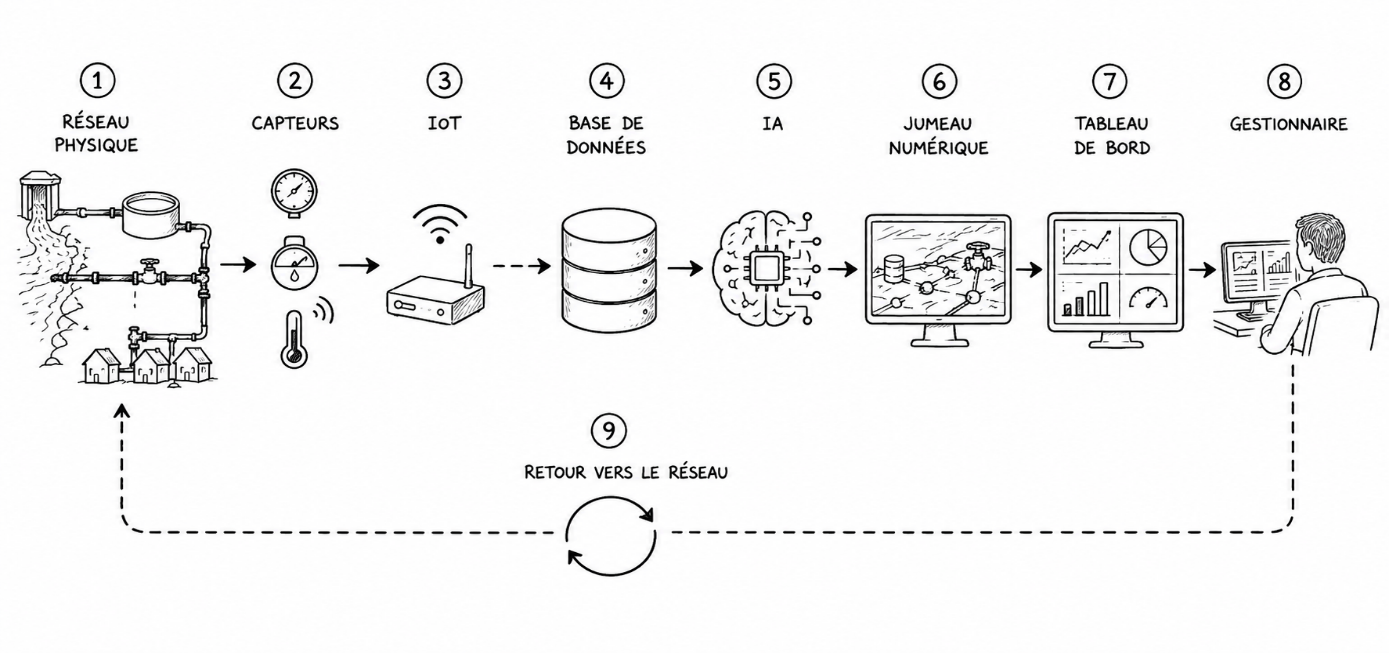
\includegraphics[width=6.3in,height=2.96522in]{figures/image2.png}

Figure 2. Architecture générale d\textquotesingle un jumeau numérique
intégrant l\textquotesingle intelligence artificielle

\subsection{\texorpdfstring{\textbf{1.10. L\textquotesingle intelligence
artificielle appliquée à la gestion des réseaux d\textquotesingle eau
potable}}{1.10. L\textquotesingle intelligence artificielle appliquée à la gestion des réseaux d\textquotesingle eau potable}}\label{lintelligence-artificielle-appliquuxe9e-uxe0-la-gestion-des-ruxe9seaux-deau-potable}

L\textquotesingle intelligence artificielle (IA) constitue
aujourd\textquotesingle hui l\textquotesingle une des technologies les
plus innovantes de la transformation numérique des infrastructures
modernes. Son développement rapide au cours des dernières décennies a
profondément modifié la manière dont les systèmes complexes sont conçus,
surveillés et gérés. Grâce aux progrès réalisés dans les domaines de la
puissance de calcul, de la disponibilité des données massives (\emph{Big
Data}), de l\textquotesingle Internet des objets (IoT) et de
l\textquotesingle informatique en nuage (\emph{Cloud Computing}),
l\textquotesingle intelligence artificielle est devenue un outil
stratégique capable d\textquotesingle analyser de grandes quantités
d\textquotesingle informations, d\textquotesingle apprendre à partir des
données et d\textquotesingle assister les décideurs dans des contextes
où les méthodes traditionnelles atteignent leurs limites.
Aujourd\textquotesingle hui, l\textquotesingle IA est utilisée dans de
nombreux secteurs tels que la santé, les transports,
l\textquotesingle industrie, la finance, l\textquotesingle agriculture,
les télécommunications ainsi que la gestion des infrastructures
urbaines, où elle contribue à améliorer les performances, réduire les
coûts d\textquotesingle exploitation et renforcer la qualité des
services \cite{ref21}.

Selon John McCarthy, qui introduisit officiellement
l\textquotesingle expression « Intelligence Artificielle » lors de la
conférence de Dartmouth en 1956, l\textquotesingle IA désigne la science
et l\textquotesingle ingénierie consistant à concevoir des machines
capables d\textquotesingle exécuter des tâches nécessitant normalement
l\textquotesingle intelligence humaine. Cette définition a
progressivement évolué avec les avancées scientifiques et
technologiques. Aujourd\textquotesingle hui,
l\textquotesingle intelligence artificielle peut être définie comme un
ensemble de méthodes, d\textquotesingle algorithmes et de modèles
informatiques permettant à une machine de percevoir son environnement,
d\textquotesingle apprendre à partir des données, de raisonner, de
prendre certaines décisions et d\textquotesingle améliorer
progressivement ses performances sans être explicitement programmée pour
chaque situation. Contrairement aux systèmes informatiques classiques
qui exécutent uniquement des instructions prédéfinies, les systèmes
fondés sur l\textquotesingle intelligence artificielle sont capables
d\textquotesingle extraire des connaissances à partir des données et
d\textquotesingle adapter leur comportement en fonction des expériences
accumulées \cite{ref67}.

L\textquotesingle évolution de l\textquotesingle intelligence
artificielle s\textquotesingle est déroulée en plusieurs étapes. Après
une période d\textquotesingle enthousiasme dans les années 1950 et 1960,
les limites des capacités informatiques disponibles ont conduit à un
ralentissement des recherches, souvent qualifié «
d\textquotesingle hiver de l\textquotesingle intelligence artificielle
». À partir des années 1990, l\textquotesingle amélioration des
performances des ordinateurs, la disponibilité croissante des données
numériques et le développement de nouveaux algorithmes
d\textquotesingle apprentissage automatique ont permis un regain
d\textquotesingle intérêt pour cette discipline. Depuis les années 2010,
l\textquotesingle essor du \emph{Deep Learning}, des processeurs
graphiques (GPU) et des plateformes de calcul distribué a
considérablement accéléré les performances des systèmes
d\textquotesingle intelligence artificielle.
Aujourd\textquotesingle hui, ces avancées permettent de résoudre des
problèmes particulièrement complexes dans des domaines tels que la
vision artificielle, la reconnaissance vocale, le traitement automatique
du langage naturel, la robotique ou encore la gestion intelligente des
infrastructures \cite{ref68}.

L\textquotesingle intelligence artificielle regroupe plusieurs branches
complémentaires répondant à des objectifs différents. Parmi celles-ci
figurent notamment le raisonnement automatisé, les systèmes experts, la
robotique, la vision par ordinateur, le traitement automatique du
langage naturel (\emph{Natural Language Processing}), ainsi que
l\textquotesingle apprentissage automatique (\emph{Machine Learning}).
Ce dernier occupe aujourd\textquotesingle hui une place centrale dans la
majorité des applications modernes de l\textquotesingle intelligence
artificielle. Il permet à un système informatique
d\textquotesingle apprendre automatiquement des relations existant dans
les données afin d\textquotesingle effectuer des prédictions, des
classifications ou des détections sans qu\textquotesingle il soit
nécessaire de programmer explicitement toutes les règles de décision.
Cette capacité d\textquotesingle apprentissage constitue
l\textquotesingle une des principales raisons expliquant
l\textquotesingle intérêt croissant porté à l\textquotesingle IA dans
les systèmes de surveillance des infrastructures critiques \cite{ref69}.

Le \textbf{Machine Learning} peut être défini comme une branche de
l\textquotesingle intelligence artificielle reposant sur des méthodes
statistiques et mathématiques permettant aux ordinateurs
d\textquotesingle améliorer progressivement leurs performances grâce à
l\textquotesingle analyse des données. Les techniques
d\textquotesingle apprentissage supervisé utilisent des exemples déjà
étiquetés afin d\textquotesingle apprendre à prédire une sortie à partir
d\textquotesingle un ensemble de variables d\textquotesingle entrée. À
l\textquotesingle inverse, les méthodes d\textquotesingle apprentissage
non supervisé cherchent à identifier automatiquement des structures ou
des regroupements dans les données sans disposer
d\textquotesingle exemples préalablement classifiés. Une troisième
catégorie, appelée apprentissage par renforcement, permet à un système
d\textquotesingle apprendre progressivement en interagissant avec son
environnement et en recevant des récompenses ou des pénalités selon les
décisions prises. Le choix de l\textquotesingle approche dépend
généralement de la nature du problème étudié et des données disponibles
\cite{ref70}.

Parmi les techniques de Machine Learning, plusieurs algorithmes
présentent un intérêt particulier pour la gestion des réseaux
d\textquotesingle eau potable. Les arbres de décision facilitent
l\textquotesingle interprétation des résultats et permettent de
classifier différentes situations de fonctionnement. Les forêts
aléatoires (\emph{Random Forest}) améliorent la robustesse des
prédictions en combinant plusieurs arbres de décision indépendants. Les
machines à vecteurs de support (\emph{Support Vector Machines -- SVM})
sont fréquemment utilisées pour la classification de données complexes,
tandis que les réseaux de neurones artificiels permettent de modéliser
des relations non linéaires particulièrement adaptées aux phénomènes
hydrauliques. Ces méthodes peuvent être exploitées pour analyser les
données issues des capteurs, détecter des comportements anormaux,
prévoir l\textquotesingle apparition de fuites ou estimer
l\textquotesingle évolution future de certains paramètres du réseau
\cite{ref71}.

Une autre évolution majeure est représentée par le \textbf{Deep
Learning}, qui constitue une sous-discipline du Machine Learning basée
sur des réseaux de neurones artificiels comportant plusieurs couches de
traitement. Grâce à cette architecture profonde, ces modèles sont
capables d\textquotesingle extraire automatiquement des caractéristiques
complexes à partir de grandes quantités de données. Le Deep Learning est
largement utilisé dans les domaines nécessitant
l\textquotesingle analyse d\textquotesingle images, de vidéos, de sons
ou de séries temporelles. Dans le contexte des infrastructures
hydrauliques, ces techniques peuvent être mobilisées pour analyser les
variations temporelles de pression ou de débit, reconnaître certains
schémas annonciateurs de défaillances ou améliorer la précision des
modèles prédictifs. Toutefois, leur mise en œuvre nécessite généralement
des volumes importants de données ainsi que des ressources de calcul
plus élevées que celles exigées par les méthodes classiques de Machine
Learning \cite{ref72}.

Dans le domaine des réseaux de distribution d\textquotesingle eau
potable, l\textquotesingle intelligence artificielle ouvre
aujourd\textquotesingle hui des perspectives importantes pour améliorer
la surveillance et la gestion des infrastructures. Les données provenant
des capteurs installés sur le réseau peuvent être analysées
automatiquement afin d\textquotesingle identifier des variations
inhabituelles de pression, des modifications de débit ou des
comportements susceptibles de révéler une fuite, une rupture de conduite
ou une défaillance d\textquotesingle un équipement. Les modèles
prédictifs permettent également d\textquotesingle estimer la probabilité
d\textquotesingle apparition de certaines pannes à partir des données
historiques, facilitant ainsi la planification des opérations de
maintenance préventive. L\textquotesingle intelligence artificielle peut
en outre contribuer à optimiser la gestion des pompes, la régulation de
la pression, la prévision de la demande en eau ou encore la réduction
des pertes d\textquotesingle eau non facturée (\emph{Non-Revenue
Water}). Ces différentes applications participent à
l\textquotesingle amélioration des performances techniques et
économiques des services d\textquotesingle approvisionnement en eau
\cite{ref73}.

Dans le cadre du présent mémoire, l\textquotesingle intelligence
artificielle constitue l\textquotesingle un des composants essentiels du
jumeau numérique proposé pour le réseau de fourniture
d\textquotesingle eau potable de la commune de Kadutu. Les données
collectées à partir des capteurs, qu\textquotesingle elles soient
réelles ou simulées dans le cadre du prototype, seront exploitées afin
d\textquotesingle entraîner un modèle de Machine Learning capable de
détecter automatiquement certaines anomalies du réseau, notamment les
baisses anormales de pression, les variations inhabituelles de débit ou
les situations pouvant traduire une fuite. Le modèle
d\textquotesingle IA pourra également assister les gestionnaires dans la
prise de décision en fournissant des alertes, des prédictions et des
recommandations concernant les opérations de maintenance. Ainsi,
l\textquotesingle intégration de l\textquotesingle intelligence
artificielle permettra au jumeau numérique de dépasser le simple rôle de
représentation virtuelle pour devenir un véritable système intelligent
d\textquotesingle aide à la décision.

L\textquotesingle intelligence artificielle apparaît donc
aujourd\textquotesingle hui comme un levier majeur de modernisation des
réseaux de distribution d\textquotesingle eau potable. Associée aux
capteurs intelligents, à l\textquotesingle Internet des objets et au
jumeau numérique, elle offre de nouvelles possibilités de surveillance,
d\textquotesingle analyse prédictive et d\textquotesingle optimisation
des infrastructures hydrauliques. Néanmoins, son efficacité dépend
largement de la qualité des données disponibles, de la pertinence des
modèles d\textquotesingle apprentissage utilisés et de leur capacité à
s\textquotesingle adapter aux spécificités du réseau étudié. Ces
considérations justifient pleinement son intégration dans
l\textquotesingle architecture du jumeau numérique développé dans le
cadre de cette recherche.

\subsection{\texorpdfstring{\textbf{1.11. Intégration du jumeau
numérique et de l\textquotesingle intelligence artificielle dans la
gestion des réseaux d\textquotesingle eau
potable}}{1.11. Intégration du jumeau numérique et de l\textquotesingle intelligence artificielle dans la gestion des réseaux d\textquotesingle eau potable}}\label{intuxe9gration-du-jumeau-numuxe9rique-et-de-lintelligence-artificielle-dans-la-gestion-des-ruxe9seaux-deau-potable}

L\textquotesingle évolution des infrastructures intelligentes a
progressivement conduit à l\textquotesingle intégration de plusieurs
technologies numériques complémentaires afin d\textquotesingle améliorer
la gestion des systèmes complexes. Parmi ces technologies, le jumeau
numérique et l\textquotesingle intelligence artificielle occupent
aujourd\textquotesingle hui une place centrale. Pris individuellement,
chacun apporte des avantages significatifs : le jumeau numérique permet
de représenter virtuellement un système physique et de suivre son
évolution en temps réel, tandis que l\textquotesingle intelligence
artificielle offre des capacités avancées d\textquotesingle analyse,
d\textquotesingle apprentissage et de prédiction. Cependant,
c\textquotesingle est leur intégration qui permet
d\textquotesingle exploiter pleinement leur potentiel en transformant
une simple représentation numérique en un système intelligent capable
d\textquotesingle observer, d\textquotesingle analyser, de prédire et de
recommander des actions adaptées aux situations rencontrées. Cette
complémentarité constitue aujourd\textquotesingle hui
l\textquotesingle un des principaux axes de recherche dans le domaine
des infrastructures intelligentes et des villes durables \cite{ref60}.

Le fonctionnement d\textquotesingle un jumeau numérique intelligent
repose sur une interaction permanente entre le monde physique et le
monde numérique. Les données issues des capteurs installés sur le réseau
sont transmises vers une plateforme numérique où elles sont stockées,
organisées et analysées. Le jumeau numérique utilise ces informations
pour mettre à jour en permanence la représentation virtuelle du réseau,
tandis que les algorithmes d\textquotesingle intelligence artificielle
exploitent simultanément ces données afin d\textquotesingle identifier
des comportements inhabituels, d\textquotesingle effectuer des
prédictions et de proposer des recommandations aux gestionnaires. Cette
architecture permet ainsi d\textquotesingle assurer une surveillance
dynamique du système tout en offrant une capacité
d\textquotesingle analyse dépassant largement les possibilités des
méthodes conventionnelles de gestion des infrastructures hydrauliques
\cite{ref37}.

L\textquotesingle intégration de l\textquotesingle intelligence
artificielle dans un jumeau numérique permet notamment
d\textquotesingle introduire une dimension \textbf{prédictive}, qui
constitue l\textquotesingle une des principales innovations de cette
technologie. Dans un système traditionnel de supervision, les opérateurs
observent principalement l\textquotesingle état actuel du réseau et
interviennent lorsqu\textquotesingle une anomalie est détectée. En
revanche, un jumeau numérique intégrant des modèles de Machine Learning
peut analyser les données historiques et les informations en temps réel
afin d\textquotesingle estimer la probabilité
d\textquotesingle apparition de certains événements futurs. Il devient
ainsi possible d\textquotesingle anticiper les risques de fuite, de
prévoir les défaillances de certains équipements,
d\textquotesingle estimer les variations de la demande en eau ou encore
d\textquotesingle identifier les zones susceptibles de présenter une
baisse de pression. Cette approche prédictive favorise une maintenance
préventive plutôt qu\textquotesingle une maintenance corrective,
contribuant ainsi à réduire les interruptions de service et les coûts
d\textquotesingle exploitation \cite{ref61}.

Dans les réseaux de distribution d\textquotesingle eau potable, cette
intégration présente de nombreux avantages opérationnels. Les données
provenant des capteurs de pression, de débit, de niveau et de qualité de
l\textquotesingle eau peuvent être analysées automatiquement afin de
détecter des anomalies qui passeraient difficilement inaperçues lors
d\textquotesingle une surveillance manuelle. Une baisse inhabituelle de
pression observée simultanément avec une augmentation du débit dans une
section particulière du réseau peut, par exemple, être interprétée par
les algorithmes comme un indicateur probable d\textquotesingle une
fuite. De même, l\textquotesingle analyse continue des données
historiques permet de reconnaître progressivement les comportements
normaux du réseau et d\textquotesingle identifier rapidement toute
déviation significative. Cette capacité d\textquotesingle analyse
automatisée améliore considérablement la réactivité des gestionnaires et
contribue à limiter les pertes d\textquotesingle eau non facturée
(\emph{Non-Revenue Water}) \cite{ref20}.

L\textquotesingle intégration du jumeau numérique et de
l\textquotesingle intelligence artificielle facilite également la
\textbf{simulation de scénarios} avant leur mise en œuvre sur le réseau
réel. Grâce à la représentation virtuelle du système, les gestionnaires
peuvent tester différentes stratégies d\textquotesingle exploitation
sans perturber le fonctionnement des infrastructures physiques. Il
devient ainsi possible de simuler la fermeture d\textquotesingle une
vanne, l\textquotesingle ajout d\textquotesingle une nouvelle conduite,
la mise en service d\textquotesingle une station de pompage ou encore
l\textquotesingle extension du réseau vers un nouveau quartier. Les
modèles d\textquotesingle intelligence artificielle peuvent ensuite
analyser les résultats de ces simulations afin
d\textquotesingle identifier la solution présentant les meilleures
performances techniques et économiques. Cette approche réduit les
risques liés aux décisions opérationnelles et améliore la planification
des investissements futurs \cite{ref17}.

Un autre avantage majeur réside dans l\textquotesingle amélioration de
l\textquotesingle{}\textbf{aide à la décision}. Les plateformes modernes
de jumeaux numériques ne se limitent plus à présenter des données sous
forme de graphiques ou de tableaux de bord. Elles sont désormais
capables de fournir des alertes intelligentes, de hiérarchiser les
incidents selon leur niveau de gravité, de recommander des interventions
prioritaires et de proposer des scénarios optimisés de maintenance. Les
gestionnaires disposent ainsi d\textquotesingle informations directement
exploitables pour orienter leurs décisions. Cette évolution contribue à
renforcer la qualité de la gouvernance des infrastructures hydrauliques
en réduisant les délais d\textquotesingle intervention et en optimisant
l\textquotesingle utilisation des ressources disponibles \cite{ref21}.

Malgré ses nombreux avantages, l\textquotesingle intégration du jumeau
numérique et de l\textquotesingle intelligence artificielle présente
également plusieurs défis. Le premier concerne la disponibilité et la
qualité des données nécessaires à l\textquotesingle entraînement des
modèles d\textquotesingle intelligence artificielle. Des données
incomplètes, bruitées ou insuffisamment représentatives peuvent réduire
considérablement les performances des algorithmes et conduire à des
prédictions peu fiables. Le second défi réside dans
l\textquotesingle interopérabilité entre les différentes technologies
composant l\textquotesingle architecture du système, notamment les
capteurs, les protocoles de communication, les bases de données, les
logiciels de modélisation et les plateformes de visualisation. Les
questions liées à la cybersécurité, à la confidentialité des données et
aux coûts de déploiement constituent également des aspects importants à
prendre en considération, particulièrement dans les pays en
développement où les ressources techniques et financières demeurent
parfois limitées \cite{ref60}.

Dans plusieurs pays, cette intégration commence déjà à produire des
résultats encourageants. Des opérateurs de réseaux d\textquotesingle eau
utilisent aujourd\textquotesingle hui des plateformes numériques
capables de surveiller en permanence leurs infrastructures, de détecter
automatiquement certaines anomalies et de planifier les opérations de
maintenance à partir de modèles prédictifs. Bien que ces initiatives
restent encore peu nombreuses en Afrique subsaharienne, elles démontrent
le potentiel considérable de cette approche pour améliorer la
performance des services publics d\textquotesingle approvisionnement en
eau. Elles constituent également des références importantes pour les
travaux de recherche visant à adapter ces technologies aux réalités des
pays en développement \cite{ref74}.

Dans le cadre du présent mémoire, cette intégration constitue le
principe fondamental de la solution proposée. Le système développé
reposera sur une architecture dans laquelle les données provenant des
capteurs alimenteront en permanence un jumeau numérique représentant le
réseau de fourniture d\textquotesingle eau potable de la commune de
Kadutu. Ces données seront analysées par un modèle
d\textquotesingle intelligence artificielle chargé de détecter
automatiquement certaines anomalies, de prédire les risques potentiels
et d\textquotesingle assister les gestionnaires dans leurs décisions de
maintenance et de déploiement du réseau. L\textquotesingle objectif
n\textquotesingle est pas seulement de représenter virtuellement les
infrastructures, mais également de créer une plateforme intelligente
capable d\textquotesingle améliorer la qualité de la surveillance, de
réduire les pertes d\textquotesingle eau et d\textquotesingle optimiser
la gestion des ressources hydrauliques.

Ainsi, l\textquotesingle intégration du jumeau numérique et de
l\textquotesingle intelligence artificielle représente
aujourd\textquotesingle hui l\textquotesingle une des approches les plus
prometteuses pour la modernisation des réseaux de distribution
d\textquotesingle eau potable. En combinant les capacités de
représentation dynamique offertes par le jumeau numérique avec les
performances analytiques de l\textquotesingle intelligence artificielle,
il devient possible de développer des systèmes capables de surveiller
les infrastructures en continu, d\textquotesingle anticiper les
défaillances et d\textquotesingle améliorer la prise de décision. Cette
approche constitue le fondement scientifique et technologique du
prototype qui sera conçu et développé dans les chapitres suivants de ce
mémoire.

\subsection{\texorpdfstring{\textbf{1.12. Revue des travaux
antérieurs}}{1.12. Revue des travaux antérieurs}}\label{revue-des-travaux-antuxe9rieurs}

La revue des travaux antérieurs constitue une étape essentielle de toute
recherche scientifique. Elle permet d\textquotesingle examiner les
connaissances déjà produites sur le sujet étudié,
d\textquotesingle identifier les principales approches méthodologiques
adoptées par les chercheurs, d\textquotesingle analyser les résultats
obtenus ainsi que les limites des études existantes. Cette démarche
contribue non seulement à éviter la duplication des recherches déjà
réalisées, mais également à mettre en évidence les lacunes scientifiques
qui justifient la conduite d\textquotesingle une nouvelle étude. Dans le
cadre de ce mémoire, la revue des travaux antérieurs porte
principalement sur les recherches relatives à
l\textquotesingle utilisation des jumeaux numériques, de
l\textquotesingle intelligence artificielle et des technologies de
l\textquotesingle Internet des objets dans la gestion des réseaux de
distribution d\textquotesingle eau potable \cite{ref75}.

Les premières applications du concept de jumeau numérique ont été
développées dans les secteurs de l\textquotesingle industrie
manufacturière, de l\textquotesingle aéronautique et de
l\textquotesingle ingénierie des systèmes complexes. Toutefois, avec
l\textquotesingle évolution des technologies numériques et
l\textquotesingle émergence des villes intelligentes, plusieurs
chercheurs ont progressivement adapté cette approche au domaine de la
gestion des infrastructures hydrauliques. Les études réalisées montrent
qu\textquotesingle un jumeau numérique permet
d\textquotesingle améliorer la représentation virtuelle des réseaux de
distribution d\textquotesingle eau, de faciliter la surveillance en
temps réel des infrastructures et d\textquotesingle optimiser les
opérations de maintenance grâce à une meilleure exploitation des données
issues des capteurs \cite{ref8}.

Parmi les travaux les plus significatifs, \textbf{Tao et al. (2019)} ont
proposé une architecture générale de jumeau numérique fondée sur
l\textquotesingle intégration des objets connectés, des bases de
données, de la modélisation numérique et de
l\textquotesingle intelligence artificielle. Les auteurs démontrent que
cette architecture permet une interaction continue entre le système
physique et sa représentation virtuelle, favorisant ainsi la
surveillance en temps réel, la simulation de scénarios et
l\textquotesingle amélioration de la prise de décision. Bien que leurs
travaux soient principalement orientés vers le secteur industriel, les
principes proposés sont aujourd\textquotesingle hui largement repris
dans le développement de jumeaux numériques appliqués aux
infrastructures urbaines, notamment les réseaux d\textquotesingle eau
potable \cite{ref17}.

Dans le domaine spécifique de la gestion de l\textquotesingle eau,
plusieurs recherches ont démontré l\textquotesingle intérêt de
l\textquotesingle intelligence artificielle pour améliorer les
performances des réseaux de distribution. \textbf{Solomatine et Ostfeld}
ont montré que les méthodes d\textquotesingle apprentissage automatique
permettent d\textquotesingle exploiter efficacement les données
historiques afin de détecter des anomalies, de prévoir les variations de
consommation et d\textquotesingle optimiser certaines opérations
hydrauliques. De même, les travaux de \textbf{Abu-Mahfouz et ses
collaborateurs} mettent en évidence l\textquotesingle apport des réseaux
intelligents d\textquotesingle eau (\emph{Smart Water Grids}) combinant
l\textquotesingle Internet des objets, les capteurs intelligents et les
techniques d\textquotesingle intelligence artificielle pour améliorer la
surveillance des infrastructures et réduire les pertes
d\textquotesingle eau non facturée (\emph{Non-Revenue Water}) \cite{ref76}.

Plus récemment, plusieurs chercheurs se sont intéressés à la combinaison
du jumeau numérique et de l\textquotesingle intelligence artificielle
dans les infrastructures hydrauliques. Les études montrent que cette
intégration permet non seulement de représenter virtuellement le réseau,
mais également de prédire certaines défaillances avant leur apparition,
d\textquotesingle optimiser les opérations de maintenance et de simuler
différents scénarios d\textquotesingle exploitation. Les modèles
prédictifs développés à partir des données collectées par les capteurs
améliorent considérablement la capacité des gestionnaires à anticiper
les incidents et à réduire les coûts d\textquotesingle exploitation. Ces
travaux confirment ainsi que l\textquotesingle association du jumeau
numérique et de l\textquotesingle intelligence artificielle constitue
aujourd\textquotesingle hui une orientation majeure des recherches sur
les infrastructures intelligentes \cite{ref61}.

En Afrique subsaharienne, les recherches consacrées aux jumeaux
numériques appliqués aux réseaux d\textquotesingle eau potable demeurent
encore relativement limitées. La majorité des travaux portent
principalement sur la télésurveillance des réseaux, la gestion des
ressources hydriques, les systèmes d\textquotesingle information
géographique ou encore l\textquotesingle utilisation de capteurs
connectés pour le suivi de certains paramètres hydrauliques. Des projets
pilotes ont été expérimentés dans plusieurs pays tels que
l\textquotesingle Afrique du Sud, le Kenya, le Rwanda et le Ghana afin
d\textquotesingle améliorer la surveillance des infrastructures
hydrauliques grâce aux technologies numériques. Cependant, peu
d\textquotesingle études proposent une intégration complète combinant
jumeau numérique, intelligence artificielle et Internet des objets dans
un même système de gestion des réseaux d\textquotesingle eau potable
\cite{ref77}.

En République Démocratique du Congo, les travaux scientifiques portant
sur la gestion intelligente des réseaux de distribution
d\textquotesingle eau potable restent encore peu nombreux. Les
recherches existantes concernent essentiellement les difficultés
d\textquotesingle accès à l\textquotesingle eau potable, les
performances des infrastructures de distribution, les pertes
d\textquotesingle eau, la qualité du service ou les problématiques de
gouvernance du secteur hydraulique. Les solutions numériques proposées
demeurent généralement limitées à l\textquotesingle utilisation de
systèmes d\textquotesingle information géographique, de bases de données
ou d\textquotesingle outils classiques de gestion. À la connaissance de
l\textquotesingle auteur, très peu de travaux académiques se sont
spécifiquement intéressés à la conception d\textquotesingle un jumeau
numérique intégrant l\textquotesingle intelligence artificielle pour
optimiser le déploiement, la surveillance et la maintenance
d\textquotesingle un réseau de fourniture d\textquotesingle eau potable
dans le contexte congolais, en particulier dans la commune de Kadutu à
Bukavu \cite{ref78}.

L\textquotesingle analyse critique des travaux recensés met en évidence
plusieurs limites. Premièrement, la plupart des recherches sont
réalisées dans des pays disposant d\textquotesingle infrastructures
numériques avancées, ce qui rend leur transposition difficile dans les
contextes caractérisés par des ressources techniques et financières
limitées. Deuxièmement, certaines études privilégient les aspects de
modélisation hydraulique sans intégrer les capacités
d\textquotesingle apprentissage de l\textquotesingle intelligence
artificielle. D\textquotesingle autres, à l\textquotesingle inverse,
développent des modèles prédictifs performants sans proposer une
représentation virtuelle dynamique du réseau. Enfin, très peu de travaux
prennent en compte simultanément les problématiques de déploiement, de
surveillance et de maintenance dans une plateforme unique adaptée aux
réalités des villes africaines en développement \cite{ref79}.

C\textquotesingle est précisément dans cette perspective que
s\textquotesingle inscrit la présente recherche. Contrairement aux
travaux antérieurs, cette étude propose de concevoir et de développer un
\textbf{jumeau numérique intégrant l\textquotesingle intelligence
artificielle} spécifiquement adapté au réseau de fourniture
d\textquotesingle eau potable de la commune de Kadutu. Le système
proposé reposera sur une architecture combinant des capteurs
intelligents (réels ou simulés), une base de données, un modèle
numérique dynamique, des algorithmes de Machine Learning et une
plateforme interactive d\textquotesingle aide à la décision.
L\textquotesingle objectif est d\textquotesingle offrir aux
gestionnaires un outil capable de représenter virtuellement le réseau,
de détecter automatiquement certaines anomalies, de prédire les risques
potentiels et d\textquotesingle améliorer les opérations de
surveillance, de maintenance et de déploiement des infrastructures
hydrauliques. Cette approche constitue ainsi une contribution
scientifique originale au regard du contexte local étudié.

\subsection{Tableau 1.1 : Synthèse comparative des principaux travaux
antérieurs}\label{tableau-1.1-synthuxe8se-comparative-des-principaux-travaux-antuxe9rieurs}

\begin{longtable}[]{@{}
  >{\raggedright\arraybackslash}p{(\columnwidth - 10\tabcolsep) * \real{0.1483}}
  >{\raggedright\arraybackslash}p{(\columnwidth - 10\tabcolsep) * \real{0.0792}}
  >{\raggedright\arraybackslash}p{(\columnwidth - 10\tabcolsep) * \real{0.1387}}
  >{\raggedright\arraybackslash}p{(\columnwidth - 10\tabcolsep) * \real{0.1982}}
  >{\raggedright\arraybackslash}p{(\columnwidth - 10\tabcolsep) * \real{0.1950}}
  >{\raggedright\arraybackslash}p{(\columnwidth - 10\tabcolsep) * \real{0.2407}}@{}}
\toprule
oalign{}
\begin{minipage}[b]{\linewidth}\raggedright
Auteur(s)
\end{minipage} & \begin{minipage}[b]{\linewidth}\raggedright
Année
\end{minipage} & \begin{minipage}[b]{\linewidth}\raggedright
Domaine d\textquotesingle étude
\end{minipage} & \begin{minipage}[b]{\linewidth}\raggedright
Contribution principale
\end{minipage} & \begin{minipage}[b]{\linewidth}\raggedright
Limites
\end{minipage} & \begin{minipage}[b]{\linewidth}\raggedright
Apport de la présente étude
\end{minipage} \\
\midrule
oalign{}
\endhead
\bottomrule
oalign{}
\endlastfoot
Grieves & 2014 & Jumeau numérique & Formalisation du concept de Digital
Twin & Approche générale, non appliquée à l\textquotesingle eau &
Application au réseau d\textquotesingle eau potable de Kadutu \\
Tao et al. & 2019 & Industrie 4.0 & Architecture générale du jumeau
numérique & Orientation industrielle & Adaptation aux infrastructures
hydrauliques \\
Fuller et al. & 2020 & Digital Twin & Technologies, défis et
perspectives & Peu d\textquotesingle applications aux pays en
développement & Prise en compte du contexte congolais \\
Abu-Mahfouz et al. & 2020 & Smart Water Grid & Gestion intelligente des
réseaux d\textquotesingle eau & Peu de modèles de jumeaux numériques &
Intégration IoT + IA + Jumeau numérique \\
Rasheed et al. & 2020 & Digital Twin & Analyse des modèles prédictifs &
Peu orienté vers la maintenance des réseaux d\textquotesingle eau &
Accent sur la maintenance prédictive et l\textquotesingle aide à la
décision \\
\end{longtable}

Tableau 1 Synthèse comparative des principaux travaux antérieur

\chapter{Cadre méthodologique et présentation du milieu d'étude}\label{chapitre-ii-cadre-muxe9thodologique-et-pruxe9sentation-du-milieu-duxe9tude}

\subsection{2.1. Introduction du
chapitre}\label{introduction-du-chapitre}

Ce deuxième chapitre présente le cadre méthodologique adopté pour la
réalisation de cette étude ainsi que le milieu dans lequel
s\textquotesingle inscrit la recherche. Après avoir exposé, dans le
chapitre précédent, les fondements théoriques relatifs aux réseaux de
distribution d\textquotesingle eau potable, au jumeau numérique et à
l\textquotesingle intelligence artificielle, il est nécessaire de
préciser la démarche scientifique retenue pour atteindre les objectifs
fixés. En effet, la qualité des résultats d\textquotesingle une
recherche dépend en grande partie de la pertinence des méthodes
utilisées pour collecter, analyser et interpréter les données. La
méthodologie constitue ainsi le cadre qui guide
l\textquotesingle ensemble du processus de recherche, depuis
l\textquotesingle identification du problème jusqu\textquotesingle à la
conception de la solution proposée \cite{ref75}.

Dans le cadre de ce mémoire, la démarche méthodologique combine
plusieurs approches complémentaires. La première consiste en une étude
documentaire permettant d\textquotesingle analyser les travaux
scientifiques, les rapports techniques et les normes relatifs aux
réseaux de distribution d\textquotesingle eau potable, aux jumeaux
numériques et à l\textquotesingle intelligence artificielle. La deuxième
repose sur une étude de terrain menée auprès des acteurs impliqués dans
la gestion du réseau de fourniture d\textquotesingle eau potable de la
commune de Kadutu, notamment à travers des observations, des entretiens
et la collecte de données techniques. Enfin, une approche de conception
informatique sera utilisée afin de développer un prototype de jumeau
numérique intégrant des techniques d\textquotesingle intelligence
artificielle destinées à optimiser le déploiement, la surveillance et la
maintenance du réseau étudié \cite{ref81}.

Ce chapitre présente également le milieu d\textquotesingle étude retenu,
à savoir la commune de Kadutu située dans la ville de Bukavu, en
République Démocratique du Congo. Cette commune connaît une croissance
démographique importante, accompagnée d\textquotesingle une augmentation
continue des besoins en eau potable. Les défis liés à la distribution de
cette ressource, notamment les pertes d\textquotesingle eau, les
interruptions de service et les difficultés de maintenance, justifient
le choix de ce terrain d\textquotesingle étude. Une description
détaillée de son contexte géographique, administratif et
socio-économique permettra de mieux comprendre les contraintes
auxquelles est confronté le réseau de distribution d\textquotesingle eau
potable \cite{ref82}.

Par ailleurs, ce chapitre expose les méthodes et techniques de collecte
des données, les outils matériels et logiciels utilisés, les besoins
fonctionnels et non fonctionnels du système proposé, ainsi que
l\textquotesingle architecture générale retenue pour le développement du
jumeau numérique. Ces éléments méthodologiques serviront de base au
chapitre suivant, consacré à la conception et au développement de la
plateforme intelligente intégrant l\textquotesingle intelligence
artificielle.

\subsection{\texorpdfstring{\textbf{2.2. Présentation du milieu
d\textquotesingle étude}}{2.2. Présentation du milieu d\textquotesingle étude}}\label{pruxe9sentation-du-milieu-duxe9tude}

\subsubsection{2.2.1. Présentation de la ville de
Bukavu}\label{pruxe9sentation-de-la-ville-de-bukavu}

La ville de Bukavu est l\textquotesingle une des principales
agglomérations urbaines de l\textquotesingle Est de la République
Démocratique du Congo (RDC). Elle est le chef-lieu de la province du
Sud-Kivu et constitue un important centre administratif, économique,
commercial et universitaire de la région. Située à
l\textquotesingle extrémité sud-ouest du lac Kivu, à la frontière avec
la République du Rwanda, Bukavu occupe une position stratégique qui
favorise les échanges commerciaux transfrontaliers ainsi que le
développement des activités économiques. Son implantation géographique
sur un relief montagneux, caractérisé par des collines et des vallées,
influence fortement l\textquotesingle organisation de son urbanisation
ainsi que la conception et l\textquotesingle exploitation de ses
infrastructures publiques, notamment celles dédiées à la distribution de
l\textquotesingle eau potable \cite{ref83}.

Créée durant la période coloniale belge, la ville de Bukavu a connu une
croissance démographique particulièrement rapide au cours des dernières
décennies. Cette évolution résulte principalement de
l\textquotesingle accroissement naturel de la population, de
l\textquotesingle exode rural et des mouvements migratoires provoqués
par les différentes crises sécuritaires qu\textquotesingle a connues la
région des Grands Lacs. Cette croissance s\textquotesingle est
accompagnée d\textquotesingle une extension progressive des quartiers
résidentiels, souvent réalisée sans une planification urbaine
suffisante. En conséquence, plusieurs infrastructures publiques,
notamment les réseaux d\textquotesingle approvisionnement en eau
potable, ne se sont pas développées au même rythme que la population, ce
qui exerce une pression croissante sur les services de base \cite{ref82}.

Sur le plan administratif, la ville de Bukavu est subdivisée en trois
communes : Ibanda, Kadutu et Bagira. Chacune de ces communes présente
des caractéristiques géographiques, démographiques et socio-économiques
particulières. La commune d\textquotesingle Ibanda concentre la majorité
des institutions administratives, financières et commerciales. La
commune de Bagira est davantage marquée par des activités résidentielles
et artisanales. Quant à la commune de Kadutu, elle se distingue par une
très forte densité de population, une urbanisation rapide et des
contraintes importantes en matière d\textquotesingle accès aux
infrastructures de base, notamment l\textquotesingle approvisionnement
en eau potable, ce qui explique son choix comme cadre de la présente
étude \cite{ref84}.

L\textquotesingle économie de Bukavu repose principalement sur le
commerce, les services, l\textquotesingle agriculture périurbaine, les
activités artisanales ainsi que le secteur informel. La présence de
plusieurs universités, hôpitaux, organisations internationales et
institutions publiques fait également de la ville un pôle régional
important. Toutefois, malgré son dynamisme économique, Bukavu demeure
confrontée à de nombreux défis liés au développement urbain. Les
difficultés d\textquotesingle accès à l\textquotesingle eau potable,
l\textquotesingle insuffisance des infrastructures
d\textquotesingle assainissement, la gestion des déchets, la mobilité
urbaine ainsi que les contraintes énergétiques figurent parmi les
principaux problèmes auxquels les autorités locales doivent faire face.
Ces défis affectent directement les conditions de vie de la population
et nécessitent la mise en œuvre de solutions innovantes fondées sur les
technologies numériques \cite{ref85}.

L\textquotesingle approvisionnement en eau potable de la ville est
principalement assuré par la REGIDESO (Régie de Distribution
d\textquotesingle Eau), établissement public chargé de la production, du
traitement et de la distribution de l\textquotesingle eau potable dans
plusieurs villes de la République Démocratique du Congo. Malgré les
efforts réalisés par cette entreprise pour améliorer la qualité du
service, la croissance démographique, le vieillissement de certaines
infrastructures, les pertes techniques dans le réseau et les contraintes
financières rendent difficile la satisfaction de la demande croissante
en eau potable. Dans certains quartiers, les interruptions de service,
les baisses de pression et les difficultés d\textquotesingle entretien
des conduites demeurent des préoccupations récurrentes \cite{ref86}.

Au regard de ces différentes caractéristiques, la ville de Bukavu
constitue un terrain d\textquotesingle étude particulièrement pertinent
pour le développement d\textquotesingle une solution numérique basée sur
un jumeau numérique intégrant l\textquotesingle intelligence
artificielle. Les défis rencontrés dans la gestion du réseau de
distribution d\textquotesingle eau potable offrent un contexte favorable
à l\textquotesingle expérimentation de nouvelles approches de
surveillance intelligente, de maintenance prédictive et
d\textquotesingle aide à la décision. Les résultats attendus de cette
recherche pourront ainsi contribuer à améliorer les performances du
réseau de distribution d\textquotesingle eau potable tout en proposant
une démarche reproductible dans d\textquotesingle autres villes de la
République Démocratique du Congo confrontées à des problématiques
similaires.

\subsubsection{2.2.2. Présentation de la commune de
Kadutu}\label{pruxe9sentation-de-la-commune-de-kadutu}

La commune de Kadutu est l\textquotesingle une des trois communes qui
composent la ville de Bukavu, chef-lieu de la province du Sud-Kivu, en
République Démocratique du Congo. Elle constitue l\textquotesingle un
des principaux centres urbains de la ville et se distingue par une forte
concentration de population ainsi qu\textquotesingle une urbanisation
particulièrement dense. Située au cœur de Bukavu, Kadutu joue un rôle
important dans les activités commerciales, artisanales et
administratives de la ville. Toutefois, cette forte densité
démographique exerce une pression considérable sur les infrastructures
publiques, notamment celles destinées à
l\textquotesingle approvisionnement en eau potable, à
l\textquotesingle assainissement et aux réseaux de transport \cite{ref84}.

Sur le plan géographique, la commune de Kadutu est localisée entre les
communes d\textquotesingle Ibanda et de Bagira. Elle est caractérisée
par un relief accidenté composé de nombreuses collines, de vallées et de
fortes pentes, caractéristiques du paysage de la ville de Bukavu. Cette
configuration topographique influence directement la conception, le
déploiement et l\textquotesingle exploitation des réseaux de
distribution d\textquotesingle eau potable. En effet, les différences
d\textquotesingle altitude entraînent des variations importantes de
pression dans les conduites, ce qui complique la distribution uniforme
de l\textquotesingle eau et augmente les risques de fuites, de ruptures
de conduites et de dysfonctionnements hydrauliques. Ces contraintes
naturelles rendent indispensable une gestion technique rigoureuse du
réseau afin de garantir une alimentation satisfaisante de
l\textquotesingle ensemble des quartiers de la commune \cite{ref82}.

La commune de Kadutu connaît depuis plusieurs années une croissance
démographique soutenue, alimentée par l\textquotesingle accroissement
naturel de la population et par les mouvements migratoires en provenance
des zones rurales environnantes. Cette augmentation rapide du nombre
d\textquotesingle habitants s\textquotesingle accompagne
d\textquotesingle une extension continue des quartiers résidentiels,
souvent réalisée sans une planification urbaine suffisante. Il en
résulte une forte demande en infrastructures de base, notamment en
matière d\textquotesingle approvisionnement en eau potable. Dans
plusieurs quartiers, les réseaux existants ne couvrent pas entièrement
les besoins de la population, ce qui oblige certains ménages à recourir
à des sources alternatives telles que les sources naturelles, les puits
ou les vendeurs d\textquotesingle eau, avec des conséquences parfois
importantes sur la santé publique \cite{ref85}.

L\textquotesingle économie locale repose principalement sur le commerce
de proximité, les activités artisanales, les petits services, les
marchés populaires et le secteur informel. La commune abrite plusieurs
établissements scolaires, centres de santé, lieux de culte et marchés
qui attirent quotidiennement une population importante. Cette
concentration des activités humaines entraîne une consommation élevée
d\textquotesingle eau potable et nécessite un fonctionnement fiable des
infrastructures hydrauliques. Cependant, les difficultés
d\textquotesingle approvisionnement observées dans certains secteurs de
la commune affectent non seulement les conditions de vie des habitants,
mais également le fonctionnement des activités économiques et des
services publics \cite{ref87}.

L\textquotesingle alimentation en eau potable de la commune est
principalement assurée par la REGIDESO, qui exploite un réseau constitué
de stations de pompage, de réservoirs, de conduites principales, de
conduites secondaires et de branchements destinés aux consommateurs.
Malgré les efforts entrepris pour améliorer la desserte, plusieurs
difficultés persistent. Parmi celles-ci figurent les pertes
d\textquotesingle eau liées aux fuites, les baisses de pression dans
certaines zones, les interruptions fréquentes du service, le
vieillissement de certaines conduites, ainsi que les difficultés de
localisation rapide des anomalies. L\textquotesingle absence
d\textquotesingle un système intégré de surveillance en temps réel
limite la capacité des équipes techniques à intervenir rapidement et à
planifier efficacement les opérations de maintenance \cite{ref86}.

Les défis rencontrés dans la gestion du réseau d\textquotesingle eau
potable de Kadutu sont accentués par plusieurs facteurs.
D\textquotesingle une part, le relief accidenté rend complexe le
maintien d\textquotesingle une pression hydraulique constante sur
l\textquotesingle ensemble du réseau. D\textquotesingle autre part,
l\textquotesingle urbanisation rapide entraîne
l\textquotesingle apparition de nouvelles zones
d\textquotesingle habitation qui ne sont pas toujours intégrées
immédiatement au réseau existant. En outre, les contraintes financières,
le coût élevé du renouvellement des infrastructures et la disponibilité
limitée des outils modernes de surveillance compliquent davantage la
gestion quotidienne du système. Ces difficultés justifient le recours à
des technologies innovantes capables d\textquotesingle améliorer la
connaissance de l\textquotesingle état du réseau et
d\textquotesingle optimiser les décisions des gestionnaires \cite{ref88}.

Dans ce contexte, la commune de Kadutu constitue un terrain
particulièrement pertinent pour l\textquotesingle expérimentation
d\textquotesingle un jumeau numérique intégrant
l\textquotesingle intelligence artificielle. Les caractéristiques du
réseau, la diversité des contraintes techniques et les besoins
croissants de la population offrent un cadre propice au développement
d\textquotesingle une solution capable de représenter virtuellement les
infrastructures, de collecter les données issues des capteurs, de
détecter automatiquement certaines anomalies et
d\textquotesingle assister les gestionnaires dans les opérations de
surveillance, de maintenance et de planification du déploiement du
réseau. Les résultats de cette recherche pourraient ainsi contribuer à
améliorer la gestion de l\textquotesingle eau potable dans la commune et
servir de modèle pour d\textquotesingle autres collectivités confrontées
à des problématiques similaires.

Enfin, le choix de la commune de Kadutu ne répond pas uniquement à des
considérations géographiques. Il s\textquotesingle inscrit également
dans une volonté scientifique de proposer une solution adaptée aux
réalités des villes africaines en développement, où les contraintes
techniques, économiques et organisationnelles nécessitent des approches
innovantes, accessibles et évolutives. Le prototype développé dans le
cadre de cette étude a ainsi pour ambition de démontrer que
l\textquotesingle intégration du jumeau numérique, de
l\textquotesingle intelligence artificielle et des technologies de
l\textquotesingle Internet des objets peut constituer un levier efficace
pour améliorer durablement la performance des réseaux de distribution
d\textquotesingle eau potable.

\section{\texorpdfstring{\textbf{2.2.3. Présentation du réseau de
fourniture d\textquotesingle eau potable de la commune de
Kadutu}}{2.2.3. Présentation du réseau de fourniture d\textquotesingle eau potable de la commune de Kadutu}}\label{pruxe9sentation-du-ruxe9seau-de-fourniture-deau-potable-de-la-commune-de-kadutu}

Le réseau de fourniture d\textquotesingle eau potable de la commune de
Kadutu fait partie du système d\textquotesingle alimentation exploité
par la Régie de Distribution d\textquotesingle Eau (REGIDESO),
entreprise publique chargée de la production, du traitement et de la
distribution de l\textquotesingle eau potable dans plusieurs villes de
la République Démocratique du Congo. Dans la ville de Bukavu, la
REGIDESO assure l\textquotesingle approvisionnement en eau des trois
communes que sont Ibanda, Kadutu et Bagira, à travers un ensemble
d\textquotesingle infrastructures hydrauliques comprenant des ouvrages
de captage, des stations de traitement, des réservoirs de stockage, des
stations de pompage, des conduites principales, des conduites
secondaires ainsi que des branchements destinés aux abonnés \cite{ref86}.

Le fonctionnement général du réseau repose sur une succession
d\textquotesingle opérations techniques permettant de garantir la
disponibilité d\textquotesingle une eau conforme aux normes de qualité
avant sa distribution aux consommateurs. L\textquotesingle eau brute est
d\textquotesingle abord captée à partir des ressources hydriques
disponibles, puis acheminée vers une station de traitement où elle subit
différentes opérations destinées à éliminer les impuretés physiques,
chimiques et microbiologiques. Après le traitement,
l\textquotesingle eau potable est stockée dans des réservoirs avant
d\textquotesingle être distribuée sous pression à travers un réseau de
conduites jusqu\textquotesingle aux différents quartiers desservis. Ce
processus nécessite une surveillance permanente afin de maintenir une
pression suffisante, d\textquotesingle assurer la continuité du service
et de préserver la qualité de l\textquotesingle eau distribuée \cite{ref4}.

Le réseau de distribution comprend plusieurs composantes essentielles
qui assurent son bon fonctionnement. Les conduites principales
transportent l\textquotesingle eau sur de longues distances depuis les
réservoirs vers les différentes zones de consommation, tandis que les
conduites secondaires assurent la desserte des quartiers et des ménages.
Des vannes de sectionnement sont installées à différents endroits afin
de permettre l\textquotesingle isolement de certaines portions du réseau
lors des opérations de maintenance ou en cas d\textquotesingle incident.
Les stations de pompage permettent d\textquotesingle assurer le
transport de l\textquotesingle eau vers les zones situées en altitude,
tandis que différents équipements de contrôle contribuent à la
régulation de la pression et du débit dans les conduites \cite{ref90}.

Dans la commune de Kadutu, le fonctionnement du réseau est fortement
influencé par les caractéristiques topographiques de la ville. Le relief
accidenté entraîne des variations importantes de pression hydraulique
selon les quartiers desservis. Les secteurs situés en altitude
connaissent fréquemment des difficultés
d\textquotesingle approvisionnement en raison d\textquotesingle une
pression insuffisante, alors que les zones basses peuvent être soumises
à des pressions plus élevées susceptibles d\textquotesingle accroître
les risques de rupture des conduites. Cette situation complique la
gestion quotidienne du réseau et nécessite une surveillance continue des
paramètres hydrauliques afin d\textquotesingle assurer une distribution
équilibrée de l\textquotesingle eau potable \cite{ref34}.

Malgré les efforts entrepris par la REGIDESO, plusieurs contraintes
techniques limitent encore les performances du réseau. Le vieillissement
progressif de certaines conduites favorise l\textquotesingle apparition
de fuites parfois difficiles à localiser. Les interruptions
d\textquotesingle alimentation électrique peuvent également perturber le
fonctionnement des stations de pompage et provoquer des interruptions de
la distribution. À cela s\textquotesingle ajoutent les difficultés
d\textquotesingle accès à certaines infrastructures, le manque
d\textquotesingle outils modernes de surveillance ainsi que la faible
disponibilité de données en temps réel sur l\textquotesingle état du
réseau. Ces contraintes rendent souvent les interventions techniques
réactives plutôt que préventives, ce qui augmente les coûts
d\textquotesingle exploitation et les pertes d\textquotesingle eau
\cite{ref92}.

L\textquotesingle un des principaux indicateurs utilisés pour évaluer la
performance d\textquotesingle un réseau de distribution est le taux
d\textquotesingle eau non facturée (Non-Revenue Water -- NRW). Cet
indicateur représente la différence entre le volume
d\textquotesingle eau produit et le volume effectivement facturé aux
consommateurs. Les pertes peuvent être d\textquotesingle origine
physique, notamment en raison des fuites ou des ruptures de conduites,
ou d\textquotesingle origine commerciale, résultant par exemple des
erreurs de comptage ou des branchements irréguliers. Selon
l\textquotesingle Association Internationale de l\textquotesingle Eau
(\emph{International Water Association -- IWA}), la réduction du taux
d\textquotesingle eau non facturée constitue aujourd\textquotesingle hui
une priorité majeure pour les exploitants des réseaux
d\textquotesingle eau potable, car elle permet
d\textquotesingle améliorer simultanément la performance technique,
économique et environnementale des services
d\textquotesingle approvisionnement \cite{ref11}.

Dans le contexte de la commune de Kadutu, la surveillance du réseau
repose encore largement sur des inspections de terrain, les signalements
des usagers et les interventions des équipes techniques après la
survenue d\textquotesingle un incident. Cette approche présente
plusieurs limites, notamment des délais importants dans la détection des
anomalies, une localisation parfois imprécise des fuites et une faible
capacité à anticiper les défaillances futures. En conséquence, certaines
anomalies peuvent persister pendant une longue période avant
d\textquotesingle être détectées, entraînant des pertes importantes
d\textquotesingle eau potable ainsi qu\textquotesingle une dégradation
progressive des infrastructures \cite{ref20}.

Face à ces difficultés, l\textquotesingle intégration des technologies
numériques apparaît comme une solution particulièrement prometteuse.
L\textquotesingle installation de capteurs intelligents mesurant en
continu la pression, le débit, le niveau des réservoirs ou encore la
qualité de l\textquotesingle eau permettrait de disposer
d\textquotesingle informations en temps réel sur le fonctionnement du
réseau. Associées à un jumeau numérique et à des algorithmes
d\textquotesingle intelligence artificielle, ces données pourraient être
exploitées pour détecter automatiquement les anomalies, simuler
différents scénarios de fonctionnement, prévoir les risques de panne et
assister les gestionnaires dans leurs décisions. Cette approche
constitue précisément la solution proposée dans le cadre du présent
mémoire afin d\textquotesingle améliorer le déploiement, la surveillance
et la maintenance du réseau de fourniture d\textquotesingle eau potable
de la commune de Kadutu.

2.3. Analyse du système existant

2.3.1. Présentation du système actuel de gestion du réseau
d\textquotesingle eau potable

Le réseau de fourniture d\textquotesingle eau potable de la commune de
Kadutu est actuellement exploité selon un mode de gestion relativement
classique, reposant essentiellement sur les infrastructures physiques
mises en place par la REGIDESO. Le fonctionnement du système
s\textquotesingle articule autour des différentes étapes de captage, de
traitement, de stockage et de distribution de l\textquotesingle eau
potable vers les abonnés. Les activités de surveillance,
d\textquotesingle exploitation et de maintenance sont principalement
assurées par les équipes techniques de la REGIDESO, qui veillent au bon
fonctionnement des installations, à la continuité du service et à la
résolution des incidents pouvant affecter le réseau \cite{ref95}.

Dans son état actuel, le réseau fonctionne principalement selon une
approche de gestion réactive. Les anomalies, telles que les fuites, les
ruptures de conduites, les baisses de pression ou les dysfonctionnements
des équipements, sont généralement détectées après leur apparition, soit
à la suite des observations effectuées par les agents de terrain, soit
après les signalements formulés par les consommateurs. Cette méthode,
bien qu\textquotesingle elle permette de résoudre les incidents,
entraîne souvent des délais importants entre
l\textquotesingle apparition du problème et son traitement effectif, ce
qui favorise l\textquotesingle augmentation des pertes
d\textquotesingle eau et la dégradation progressive des infrastructures
\cite{ref90}.

Les données relatives au fonctionnement du réseau sont majoritairement
collectées de manière manuelle. Les informations proviennent des relevés
effectués sur les équipements, des rapports
d\textquotesingle intervention des équipes techniques, des observations
réalisées lors des opérations de maintenance ainsi que des réclamations
formulées par les abonnés. Cette méthode de collecte présente plusieurs
limites, notamment l\textquotesingle absence de mise à jour en temps
réel, le risque d\textquotesingle erreurs humaines et la difficulté
d\textquotesingle obtenir une vision globale et instantanée de
l\textquotesingle état du réseau \cite{ref4}.

Par ailleurs, les décisions concernant les opérations de maintenance
reposent essentiellement sur l\textquotesingle expérience des
techniciens et sur les constats réalisés sur le terrain. Les
interventions sont généralement déclenchées après la survenue
d\textquotesingle un incident plutôt qu\textquotesingle à partir
d\textquotesingle une analyse prédictive des risques de défaillance.
Cette approche corrective entraîne des coûts élevés
d\textquotesingle exploitation, des interruptions de service parfois
prolongées ainsi qu\textquotesingle une diminution de la durée de vie
des infrastructures hydrauliques \cite{ref98}.

Dans ce contexte, l\textquotesingle absence d\textquotesingle un système
intelligent capable de centraliser les données, de surveiller en continu
les paramètres hydrauliques et d\textquotesingle anticiper les anomalies
constitue l\textquotesingle une des principales limites du système
actuel. Les progrès réalisés dans les domaines de
l\textquotesingle Internet des objets, des jumeaux numériques et de
l\textquotesingle intelligence artificielle offrent
aujourd\textquotesingle hui des solutions susceptibles de répondre
efficacement à ces insuffisances en permettant une gestion proactive du
réseau \cite{ref60}.

2.3.2. Limites du système existant

L\textquotesingle analyse du fonctionnement actuel du réseau met en
évidence plusieurs insuffisances techniques, organisationnelles et
technologiques qui réduisent les performances globales du système de
distribution d\textquotesingle eau potable.

La première limite concerne l\textquotesingle absence
d\textquotesingle une surveillance en temps réel. Les paramètres
essentiels du réseau, notamment la pression, le débit, le niveau des
réservoirs et la qualité de l\textquotesingle eau, ne sont pas suivis de
manière continue. Cette situation retarde considérablement la détection
des anomalies et augmente le temps nécessaire à leur prise en charge
\cite{ref20}.

La deuxième limite réside dans la difficulté de détecter rapidement les
fuites. Dans de nombreux cas, les fuites souterraines restent invisibles
pendant plusieurs jours, voire plusieurs semaines, avant
d\textquotesingle être identifiées. Cette situation entraîne
d\textquotesingle importantes pertes d\textquotesingle eau, une
augmentation des coûts d\textquotesingle exploitation ainsi
qu\textquotesingle une diminution du rendement global du réseau
\cite{ref11}.

Une autre faiblesse importante concerne l\textquotesingle absence de
maintenance prédictive. Les interventions sont généralement réalisées
après la survenue des pannes. Or, une stratégie de maintenance
préventive ou prédictive permettrait d\textquotesingle intervenir avant
que les équipements ne deviennent défaillants, réduisant ainsi les
interruptions de service et les dépenses liées aux réparations
d\textquotesingle urgence \cite{ref100}.

Le système actuel présente également une faible capacitée
d\textquotesingle aide à la décision. Les responsables du réseau
disposent principalement d\textquotesingle informations issues des
rapports techniques et des observations de terrain, sans outils avancés
d\textquotesingle analyse ou de simulation. Il leur est donc difficile
d\textquotesingle évaluer rapidement les conséquences
d\textquotesingle une panne, de prévoir l\textquotesingle évolution
d\textquotesingle une anomalie ou de tester différents scénarios avant
d\textquotesingle effectuer une intervention \cite{ref37}.

Enfin, l\textquotesingle absence d\textquotesingle une représentation
numérique dynamique du réseau constitue une limitation majeure. Les
infrastructures physiques ne disposent pas d\textquotesingle un modèle
virtuel capable de reproduire en temps réel leur état de fonctionnement.
Cette situation limite fortement les possibilités de simulation,
d\textquotesingle analyse prédictive et d\textquotesingle optimisation
des opérations de maintenance \cite{ref61}.

L\textquotesingle ensemble de ces insuffisances montre que le système
actuel ne répond plus pleinement aux exigences d\textquotesingle une
gestion moderne des infrastructures hydrauliques. Elles justifient le
recours à une solution intégrant un jumeau numérique, des capteurs
intelligents et des techniques d\textquotesingle intelligence
artificielle afin d\textquotesingle améliorer le déploiement, la
surveillance et la maintenance du réseau de fourniture
d\textquotesingle eau potable de la commune de Kadutu.

\section{\texorpdfstring{\textbf{2.4. Méthodologie de
recherche}}{2.4. Méthodologie de recherche}}\label{muxe9thodologie-de-recherche}

La méthodologie de recherche constitue l\textquotesingle ensemble des
démarches scientifiques, des méthodes et des techniques mises en œuvre
afin de répondre de manière rigoureuse à la problématique de recherche
et d\textquotesingle atteindre les objectifs fixés. Elle permet
d\textquotesingle organiser le processus de collecte,
d\textquotesingle analyse et d\textquotesingle interprétation des
données tout en garantissant la validité scientifique des résultats
obtenus. Selon Creswell, une méthodologie bien définie constitue un
élément fondamental de toute recherche scientifique, car elle assure la
cohérence entre la problématique, les hypothèses, les objectifs et les
résultats attendus \cite{ref75}.

Dans le cadre de cette étude portant sur la conception et le
développement d\textquotesingle un jumeau numérique intégrant
l\textquotesingle intelligence artificielle pour optimiser le
déploiement, la surveillance et la maintenance du réseau de fourniture
d\textquotesingle eau potable de la commune de Kadutu, une approche
méthodologique mixte a été retenue. Cette approche combine des méthodes
qualitatives, quantitatives et une démarche de conception informatique
afin d\textquotesingle obtenir une compréhension complète du problème
étudié et de développer une solution adaptée au contexte local.
L\textquotesingle utilisation d\textquotesingle une approche mixte est
particulièrement pertinente lorsqu\textquotesingle une recherche vise à
la fois l\textquotesingle analyse d\textquotesingle un phénomène réel et
la conception d\textquotesingle un système informatique innovant
\cite{ref100}.

La première étape de cette méthodologie consiste en une recherche
documentaire. Cette phase a permis de consulter des ouvrages
scientifiques, des articles publiés dans des revues internationales, des
rapports techniques, des normes ainsi que des documents institutionnels
portant sur les réseaux de distribution d\textquotesingle eau potable,
les technologies de l\textquotesingle Internet des objets (IoT), les
jumeaux numériques, l\textquotesingle intelligence artificielle et la
maintenance prédictive. Cette revue documentaire a servi à construire le
cadre théorique de l\textquotesingle étude, à identifier les travaux
déjà réalisés dans ce domaine et à mettre en évidence les limites des
solutions existantes \cite{ref104}.

La deuxième étape repose sur une étude de terrain réalisée dans la
commune de Kadutu. Cette phase vise à comprendre le fonctionnement réel
du réseau de distribution d\textquotesingle eau potable ainsi que les
difficultés rencontrées par les acteurs impliqués dans sa gestion. Les
informations seront obtenues grâce à des observations directes des
infrastructures, à l\textquotesingle analyse des documents techniques
disponibles, à des entretiens avec les responsables et techniciens de la
REGIDESO ainsi qu\textquotesingle à la collecte de données relatives au
fonctionnement du réseau. Cette démarche permettra
d\textquotesingle identifier les besoins fonctionnels et techniques
auxquels devra répondre le système proposé \cite{ref75}.

La troisième étape correspond à la phase de conception informatique. Sur
la base des besoins identifiés, une architecture générale du système
sera élaborée en utilisant les principes du génie logiciel. Cette étape
comprendra notamment la modélisation des processus, la conception de la
base de données, la définition de l\textquotesingle architecture
logicielle, l\textquotesingle identification des différents modules
fonctionnels ainsi que la conception des interfaces utilisateur. Les
diagrammes UML seront utilisés afin de représenter clairement les
interactions entre les différents composants du système et de faciliter
son développement \cite{ref105}.

La quatrième étape concerne le développement du prototype du jumeau
numérique. Le système sera développé sous forme d\textquotesingle une
application web moderne utilisant React.js avec Vite (JSX) pour
l\textquotesingle interface utilisateur, Python (FastAPI) pour les
services backend, SQLite ou PostgreSQL pour la gestion des données et
Axios pour les échanges entre le client et le serveur. Le prototype
intégrera un modèle numérique représentant le réseau de distribution
d\textquotesingle eau potable, un système de gestion des données issues
des capteurs ainsi qu\textquotesingle un module
d\textquotesingle intelligence artificielle destiné à analyser les
informations collectées, détecter les anomalies et produire des
prédictions relatives au fonctionnement du réseau \cite{ref106}.

Enfin, une phase de tests et d\textquotesingle évaluation sera réalisée
afin de vérifier le bon fonctionnement du système développé. Cette étape
comprendra les tests unitaires, les tests d\textquotesingle intégration,
les tests fonctionnels ainsi que des simulations de différents scénarios
de fonctionnement du réseau. Les performances du système seront évaluées
à partir de plusieurs indicateurs, notamment le temps de détection des
anomalies, la rapidité de mise à jour des données, la précision des
prédictions générées par l\textquotesingle intelligence artificielle
ainsi que la capacité du jumeau numérique à représenter fidèlement le
comportement du réseau physique. Les résultats obtenus permettront de
vérifier si la solution proposée répond effectivement aux objectifs
fixés par cette recherche \cite{ref107}.

Ainsi, la méthodologie retenue combine les exigences de la recherche
scientifique et celles du développement informatique. Elle garantit une
démarche structurée allant de l\textquotesingle analyse du problème
jusqu\textquotesingle à la validation du prototype développé. Cette
approche permettra de proposer une solution innovante, adaptée au
contexte de la commune de Kadutu et susceptible de contribuer à la
modernisation de la gestion des réseaux de distribution
d\textquotesingle eau potable.

\section{\texorpdfstring{\textbf{2.5. Méthodes et techniques de collecte
des
données}}{2.5. Méthodes et techniques de collecte des données}}\label{muxe9thodes-et-techniques-de-collecte-des-donnuxe9es}

La collecte des données constitue une étape essentielle dans toute
recherche scientifique, car elle permet de réunir les informations
nécessaires à la compréhension du problème étudié et à la validation des
hypothèses formulées. Dans le cadre de cette étude portant sur la
conception et le développement d\textquotesingle un jumeau numérique
intégrant l\textquotesingle intelligence artificielle pour optimiser le
déploiement, la surveillance et la maintenance du réseau de fourniture
d\textquotesingle eau potable de la commune de Kadutu, plusieurs
méthodes et techniques complémentaires ont été retenues afin de garantir
la fiabilité et la pertinence des données exploitées.
L\textquotesingle association de plusieurs approches permet également de
réduire les biais liés à l\textquotesingle utilisation
d\textquotesingle une seule source d\textquotesingle information et
d\textquotesingle obtenir une vision plus complète de la réalité étudiée
\cite{ref75}.

\subsection{\texorpdfstring{\textbf{2.5.1. Méthodes de
recherche}}{2.5.1. Méthodes de recherche}}\label{muxe9thodes-de-recherche}

\subsubsection{a) La méthode
analytique}\label{a-la-muxe9thode-analytique}

La méthode analytique consiste à décomposer un phénomène complexe en
différents éléments afin d\textquotesingle en comprendre le
fonctionnement, les interactions et les causes des problèmes observés.
Dans le cadre de cette recherche, cette méthode a permis
d\textquotesingle étudier le fonctionnement du réseau de distribution
d\textquotesingle eau potable de la commune de Kadutu en identifiant les
différents composants qui le constituent, notamment les ouvrages de
captage, les stations de traitement, les réservoirs, les conduites, les
équipements de pompage ainsi que les dispositifs de distribution.
L\textquotesingle analyse de ces éléments a facilité
l\textquotesingle identification des insuffisances du système actuel et
la définition des besoins auxquels devra répondre le jumeau numérique
proposé \cite{ref108}.

\subsubsection{b) La méthode
systémique}\label{b-la-muxe9thode-systuxe9mique}

La méthode systémique considère le réseau de distribution
d\textquotesingle eau potable comme un système composé de plusieurs
sous-systèmes interconnectés qui interagissent en permanence. Toute
modification apportée à un élément du réseau peut avoir des conséquences
sur l\textquotesingle ensemble du système. Cette approche est
particulièrement adaptée à la présente étude, car le jumeau numérique
devra représenter fidèlement les interactions entre les différentes
composantes du réseau afin de permettre des simulations réalistes et une
meilleure prise de décision. L\textquotesingle approche systémique
facilite également l\textquotesingle intégration des technologies
numériques, des capteurs intelligents et des algorithmes
d\textquotesingle intelligence artificielle dans un environnement unique
de gestion \cite{ref109}.

\subsubsection{c) La méthode de
conception}\label{c-la-muxe9thode-de-conception}

Étant donné que cette recherche aboutit au développement
d\textquotesingle une solution informatique, la méthode de conception
occupe une place centrale dans la démarche méthodologique. Cette méthode
consiste à analyser les besoins des utilisateurs, concevoir
l\textquotesingle architecture du système, modéliser les différents
processus et développer un prototype répondant aux exigences
fonctionnelles identifiées. Elle permettra de transformer les résultats
de l\textquotesingle analyse du système existant en une plateforme
numérique capable de représenter virtuellement le réseau
d\textquotesingle eau potable et d\textquotesingle intégrer les
mécanismes d\textquotesingle intelligence artificielle nécessaires à son
fonctionnement \cite{ref106}.

\subsection{\texorpdfstring{\textbf{2.5.2. Techniques de collecte des
données}}{2.5.2. Techniques de collecte des données}}\label{techniques-de-collecte-des-donnuxe9es}

\subsubsection{a) L\textquotesingle observation
directe}\label{a-lobservation-directe}

L\textquotesingle observation directe consiste à examiner sur le terrain
le fonctionnement réel du réseau de distribution d\textquotesingle eau
potable. Cette technique permettra d\textquotesingle observer les
différentes infrastructures exploitées par la REGIDESO, notamment les
conduites, les réservoirs, les stations de pompage ainsi que les
équipements utilisés pour la surveillance et la maintenance. Elle
permettra également d\textquotesingle identifier les contraintes
techniques rencontrées par les équipes chargées de
l\textquotesingle exploitation du réseau et de mieux comprendre les
difficultés liées aux interventions sur le terrain \cite{ref110}.

\subsubsection{b) L\textquotesingle entretien}\label{b-lentretien}

Des entretiens semi-directifs seront réalisés avec les responsables et
les techniciens de la REGIDESO afin de recueillir des informations
détaillées sur le fonctionnement du réseau, les procédures de
maintenance, les principales causes de pannes, les difficultés
rencontrées lors des interventions ainsi que les besoins exprimés en
matière de modernisation des outils de gestion. Ces entretiens
permettront également d\textquotesingle obtenir des informations qui ne
figurent pas nécessairement dans les documents techniques disponibles
\cite{ref104}.

\subsubsection{c) L\textquotesingle analyse
documentaire}\label{c-lanalyse-documentaire}

L\textquotesingle analyse documentaire portera sur les rapports
techniques de la REGIDESO, les documents administratifs, les plans du
réseau, les rapports d\textquotesingle intervention, les publications
scientifiques, les normes internationales ainsi que les différents
travaux de recherche portant sur les réseaux de distribution
d\textquotesingle eau potable, les jumeaux numériques et
l\textquotesingle intelligence artificielle. Cette technique permettra
de compléter les informations obtenues sur le terrain et
d\textquotesingle assurer une meilleure compréhension du contexte de
l\textquotesingle étude \cite{ref81}.

\subsubsection{d) La collecte des données
techniques}\label{d-la-collecte-des-donnuxe9es-techniques}

La présente étude exploitera également des données techniques relatives
au fonctionnement du réseau de distribution d\textquotesingle eau
potable. Ces données pourront concerner la pression de
l\textquotesingle eau, le débit, le niveau des réservoirs, la qualité de
l\textquotesingle eau, les historiques de pannes, les interventions de
maintenance ainsi que les informations provenant des capteurs intégrés
au prototype développé. Ces données constitueront la base de
fonctionnement du jumeau numérique et permettront
d\textquotesingle alimenter les modèles d\textquotesingle intelligence
artificielle chargés de détecter les anomalies et de produire des
prédictions \cite{ref20}.

\subsection{\texorpdfstring{\textbf{2.5.3. Population
d\textquotesingle étude}}{2.5.3. Population d\textquotesingle étude}}\label{population-duxe9tude}

La population concernée par cette recherche est constituée des acteurs
impliqués dans la gestion et l\textquotesingle utilisation du réseau de
fourniture d\textquotesingle eau potable de la commune de Kadutu. Elle
comprend principalement les responsables administratifs et techniques de
la REGIDESO, les agents chargés de l\textquotesingle exploitation et de
la maintenance du réseau ainsi que certains abonnés bénéficiant du
service de distribution d\textquotesingle eau potable. Ces différents
acteurs constituent des sources importantes
d\textquotesingle informations pour l\textquotesingle identification des
besoins fonctionnels du système proposé \cite{ref112}.

\subsection{\texorpdfstring{\textbf{2.5.4.
Échantillonnage}}{2.5.4. Échantillonnage}}\label{uxe9chantillonnage}

Compte tenu du caractère appliqué de cette recherche, un échantillonnage
raisonné (ou par choix raisonné) sera privilégié. Cette méthode consiste
à sélectionner les personnes les plus susceptibles de fournir des
informations pertinentes sur le fonctionnement du réseau étudié. Les
responsables techniques de la REGIDESO, les agents de maintenance ainsi
que les gestionnaires du réseau seront retenus en priorité en raison de
leur expérience et de leur connaissance approfondie des infrastructures
hydrauliques de la commune de Kadutu \cite{ref113}.

\subsection{\texorpdfstring{\textbf{2.5.5. Instruments de collecte des
données}}{2.5.5. Instruments de collecte des données}}\label{instruments-de-collecte-des-donnuxe9es}

Afin d\textquotesingle assurer une collecte rigoureuse des informations,
plusieurs instruments seront utilisés :

\begin{itemize}
\item
  une grille d\textquotesingle observation destinée à relever les
  caractéristiques des infrastructures et les anomalies observées sur le
  terrain ;
\item
  un guide d\textquotesingle entretien semi-directif pour orienter les
  échanges avec les responsables et les techniciens de la REGIDESO ;
\item
  une fiche de collecte des données techniques permettant
  d\textquotesingle enregistrer les paramètres hydrauliques nécessaires
  au fonctionnement du jumeau numérique ;
\item
  des documents techniques (rapports d\textquotesingle exploitation,
  schémas du réseau, historiques des interventions et données
  statistiques) mis à disposition par la REGIDESO ;
\item
  les données générées par le prototype développé dans le cadre de cette
  étude, notamment les mesures simulées de pression, de débit, de niveau
  d\textquotesingle eau et les alertes produites par les algorithmes
  d\textquotesingle intelligence artificielle \cite{ref107}.
\end{itemize}

L\textquotesingle utilisation combinée de ces différents instruments
permettra de garantir la qualité des informations recueillies et
d\textquotesingle assurer une base de données fiable pour la conception,
le développement et l\textquotesingle évaluation du jumeau numérique
proposé.

\section{\texorpdfstring{\textbf{2.6. Outils matériels et logiciels
utilisés}}{2.6. Outils matériels et logiciels utilisés}}\label{outils-matuxe9riels-et-logiciels-utilisuxe9s}

La réalisation d\textquotesingle un système informatique intégrant un
jumeau numérique, des technologies de l\textquotesingle Internet des
objets (IoT) et des techniques d\textquotesingle intelligence
artificielle nécessite la mise en œuvre d\textquotesingle un ensemble
cohérent de ressources matérielles et logicielles. Ces ressources
permettent d\textquotesingle assurer les différentes étapes du projet,
depuis l\textquotesingle analyse des besoins jusqu\textquotesingle au
développement, aux tests et à l\textquotesingle évaluation du prototype.
Le choix des outils retenus dans cette étude repose sur plusieurs
critères, notamment leurs performances, leur fiabilité, leur facilité
d\textquotesingle intégration, leur caractère open source ainsi que leur
large adoption par la communauté scientifique et les développeurs.
L\textquotesingle utilisation de technologies modernes garantit
également la possibilité de faire évoluer le système vers une solution
opérationnelle pouvant être déployée à plus grande échelle \cite{ref106}.

\subsection{\texorpdfstring{\textbf{2.6.1. Outils
matériels}}{2.6.1. Outils matériels}}\label{outils-matuxe9riels}

Le développement et les tests du système proposé nécessitent un
environnement matériel capable de supporter les opérations de
programmation, d\textquotesingle exécution des modèles
d\textquotesingle intelligence artificielle et de simulation du réseau
de distribution d\textquotesingle eau potable. À cet effet, un
ordinateur personnel constitue la principale plateforme de
développement.

Les caractéristiques matérielles minimales retenues sont les suivantes :

\begin{longtable}[]{@{}
  >{\raggedright\arraybackslash}p{(\columnwidth - 2\tabcolsep) * \real{0.2440}}
  >{\raggedright\arraybackslash}p{(\columnwidth - 2\tabcolsep) * \real{0.7560}}@{}}
\toprule
oalign{}
\begin{minipage}[b]{\linewidth}\raggedright
Élément
\end{minipage} & \begin{minipage}[b]{\linewidth}\raggedright
Caractéristiques recommandées
\end{minipage} \\
\midrule
oalign{}
\endhead
\bottomrule
oalign{}
\endlastfoot
Processeur & Intel Core i5 (8ᵉ génération ou supérieur) ou AMD Ryzen
5 \\
Mémoire vive (RAM) & 8 Go minimum (16 Go recommandés) \\
Stockage & SSD 256 Go ou supérieur \\
Système d\textquotesingle exploitation & Windows 11 ou Ubuntu Linux
22.04 LTS \\
Connexion Internet & Requise pour l\textquotesingle installation des
bibliothèques, la documentation et les mises à jour \\
\end{longtable}

Tableau 2 Outils matériels

Ces caractéristiques permettent d\textquotesingle exécuter simultanément
les différents composants du système, notamment le serveur backend,
l\textquotesingle interface web, la base de données et les bibliothèques
d\textquotesingle intelligence artificielle, tout en assurant de bonnes
performances lors des simulations \cite{ref114}.

\subsection{\texorpdfstring{\textbf{2.6.2. Outils
logiciels}}{2.6.2. Outils logiciels}}\label{outils-logiciels}

\subsubsection{a) React.js avec Vite
(JSX)}\label{a-react.js-avec-vite-jsx}

L\textquotesingle interface utilisateur du jumeau numérique est
développée avec React.js, une bibliothèque JavaScript open source créée
par Meta pour la conception d\textquotesingle interfaces utilisateur
interactives et réactives. React repose sur une architecture basée sur
des composants réutilisables, facilitant le développement
d\textquotesingle applications web modernes. Afin
d\textquotesingle améliorer les performances de développement, le projet
utilise Vite comme outil de construction (\emph{build tool}), offrant un
démarrage rapide du serveur de développement, un rechargement instantané
des modifications (\emph{Hot Module Replacement}) et une optimisation
efficace des fichiers lors de la compilation. Contrairement à la version
TypeScript, l\textquotesingle ensemble du projet est développé en
JavaScript (JSX), conformément aux choix techniques retenus dans cette
étude \cite{ref115}.

\subsubsection{b) FastAPI}\label{b-fastapi}

Le serveur applicatif est développé avec FastAPI, un framework moderne
de Python destiné à la création d\textquotesingle API REST performantes.
FastAPI facilite la communication entre l\textquotesingle interface
React.js, la base de données et les modules
d\textquotesingle intelligence artificielle. Il offre également une
documentation automatique des API grâce à OpenAPI (Swagger), ce qui
simplifie les tests et l\textquotesingle intégration des différents
composants du système \cite{ref116}.

\subsubsection{c) Python}\label{c-python}

Le langage Python est utilisé pour le développement du backend ainsi que
pour l\textquotesingle implémentation des algorithmes
d\textquotesingle intelligence artificielle. Son vaste écosystème de
bibliothèques spécialisées dans l\textquotesingle analyse de données,
l\textquotesingle apprentissage automatique et le calcul scientifique en
fait l\textquotesingle un des langages les plus utilisés dans les
projets d\textquotesingle intelligence artificielle. Python assure
également le traitement des données provenant des capteurs, la
simulation de certaines variables hydrauliques et la génération des
prédictions relatives au fonctionnement du réseau \cite{ref117}.

\subsubsection{d) Base de données
SQLite}\label{d-base-de-donnuxe9es-sqlite}

Les données relatives aux capteurs, aux équipements du réseau, aux
alertes générées par le système ainsi qu\textquotesingle aux historiques
de fonctionnement sont stockées dans une base de données SQLite. Ce
système de gestion de base de données relationnelle présente
l\textquotesingle avantage d\textquotesingle être léger, rapide et
facile à intégrer dans un prototype de recherche. Il ne nécessite pas
l\textquotesingle installation d\textquotesingle un serveur dédié et
permet une gestion efficace des données locales. Son utilisation est
particulièrement adaptée au développement d\textquotesingle un prototype
académique avant une éventuelle migration vers PostgreSQL ou MySQL dans
un environnement de production \cite{ref118}.

\subsubsection{e) Leaflet.js}\label{e-leaflet.js}

La représentation cartographique du réseau de distribution
d\textquotesingle eau potable est réalisée à l\textquotesingle aide de
Leaflet.js, une bibliothèque JavaScript open source spécialisée dans les
cartes interactives. Leaflet permet de visualiser les conduites, les
réservoirs, les stations de pompage, les capteurs ainsi que les
différentes zones desservies par le réseau. Les informations provenant
du backend sont affichées en temps réel sur la carte, offrant aux
gestionnaires une représentation dynamique du fonctionnement du réseau
\cite{ref119}.

\subsubsection{f) Bibliothèques d\textquotesingle intelligence
artificielle}\label{f-bibliothuxe8ques-dintelligence-artificielle}

L\textquotesingle intelligence artificielle est développée à
l\textquotesingle aide de plusieurs bibliothèques Python spécialisées
dans l\textquotesingle analyse des données et
l\textquotesingle apprentissage automatique :

\begin{itemize}
\item
  NumPy : calcul scientifique et manipulation des tableaux numériques.
\item
  Pandas : traitement et organisation des données.
\item
  Scikit-learn : développement des modèles de Machine Learning,
  notamment pour la détection des anomalies et la prédiction des pannes.
\item
  Joblib : sauvegarde et chargement des modèles entraînés.
\end{itemize}

Ces bibliothèques permettent d\textquotesingle exploiter efficacement
les données collectées afin d\textquotesingle améliorer les capacités
prédictives du jumeau numérique \cite{ref120}.

\subsubsection{g) Visual Studio Code}\label{g-visual-studio-code}

Le développement du système est réalisé avec Visual Studio Code, un
environnement de développement intégré (IDE) reconnu pour sa légèreté,
ses nombreuses extensions et son excellente compatibilité avec
JavaScript, Python et React.js. Il facilite la programmation, le
débogage et la gestion des différentes composantes du projet \cite{ref121}.

\subsubsection{h) Git et GitHub}\label{h-git-et-github}

Afin d\textquotesingle assurer le suivi des modifications du code source
et la gestion des différentes versions du projet, les outils Git et
GitHub sont utilisés. Ils permettent de sauvegarder
l\textquotesingle évolution du développement, de collaborer efficacement
avec d\textquotesingle autres développeurs et de garantir la traçabilité
des modifications apportées au système \cite{ref122}.

\subsection{\texorpdfstring{\textbf{2.6.3. Justification du choix des
outils}}{2.6.3. Justification du choix des outils}}\label{justification-du-choix-des-outils}

Les technologies retenues dans cette étude répondent aux exigences
fonctionnelles et techniques du projet. React.js offre une interface
utilisateur moderne et interactive, FastAPI assure une communication
rapide entre les différents modules, Python facilite
l\textquotesingle intégration des algorithmes
d\textquotesingle intelligence artificielle tandis que SQLite permet une
gestion simple et efficace des données du prototype.
L\textquotesingle utilisation de Leaflet garantit une représentation
cartographique dynamique du réseau d\textquotesingle eau potable,
indispensable à la mise en œuvre du jumeau numérique. Enfin, les
bibliothèques d\textquotesingle apprentissage automatique offrent les
capacités nécessaires à la détection des anomalies, à la prédiction des
pannes et à l\textquotesingle assistance des gestionnaires dans leurs
prises de décision. L\textquotesingle ensemble de ces outils constitue
une architecture logicielle cohérente, évolutive et adaptée aux
objectifs de la présente recherche.

\subsubsection{2.7. Analyse des besoins du
système}\label{analyse-des-besoins-du-systuxe8me}

L\textquotesingle analyse des besoins constitue une étape essentielle
dans le processus de conception d\textquotesingle un système
informatique. Elle permet d\textquotesingle identifier les
fonctionnalités attendues par les utilisateurs ainsi que les contraintes
techniques auxquelles le système devra répondre. Dans le cadre de cette
étude, cette analyse est réalisée sur la base des insuffisances
observées dans le système actuel de gestion du réseau de fourniture
d\textquotesingle eau potable de la commune de Kadutu ainsi que des
objectifs définis par la recherche. Les besoins identifiés serviront de
référence pour la conception et le développement du jumeau numérique
intégrant l\textquotesingle intelligence artificielle \cite{ref106}.

\subsubsection{2.7.1. Besoins fonctionnels}\label{besoins-fonctionnels}

Les besoins fonctionnels représentent les services que le système devra
offrir à ses utilisateurs. Ils décrivent les différentes fonctions que
l\textquotesingle application devra exécuter afin de répondre aux
attentes des gestionnaires du réseau d\textquotesingle eau potable
\cite{ref114}.

\begin{itemize}
\item
  Représenter numériquement le réseau...
\item
  Afficher les données des capteurs...
\item
  Détecter les anomalies...
\item
  ...
\end{itemize}

\subsubsection{2.7.2. Besoins non
fonctionnels}\label{besoins-non-fonctionnels}

Les besoins non fonctionnels définissent les critères de qualité du
système, notamment les performances, la sécurité, la disponibilité, la
fiabilité et la facilité de maintenance. Ces exigences garantissent un
fonctionnement efficace et durable de l\textquotesingle application
\cite{ref123}.

\subsubsection{2.7.3. Identification des
acteurs}\label{identification-des-acteurs}

L\textquotesingle identification des acteurs permet de définir les
différentes entités qui interagiront avec le système. Cette étape est
indispensable pour la modélisation UML, notamment lors de
l\textquotesingle élaboration du diagramme de cas
d\textquotesingle utilisation.

\subsubsection{\texorpdfstring{
Administrateur}{ Administrateur}}\label{administrateur}

Il assure la gestion générale de la plateforme. Il peut créer des
comptes utilisateurs, gérer les paramètres du système, administrer les
équipements et superviser le fonctionnement global du jumeau numérique.

\subsubsection{Gestionnaire du réseau}\label{gestionnaire-du-ruxe9seau}

Il consulte les informations relatives au réseau, visualise les alertes,
suit les indicateurs de performance et prend les décisions nécessaires
concernant l\textquotesingle exploitation et la maintenance.

\subsubsection{Technicien de
maintenance}\label{technicien-de-maintenance}

Il reçoit les alertes générées par le système, consulte la localisation
des anomalies, enregistre les interventions réalisées et met à jour
l\textquotesingle état des équipements.

\subsubsection{Capteurs IoT}\label{capteurs-iot}

Les capteurs constituent des acteurs externes du système. Ils
transmettent automatiquement les données de pression, de débit, de
niveau, de qualité de l\textquotesingle eau ainsi que les informations
relatives au fonctionnement des équipements.

\subsection{\texorpdfstring{\textbf{2.7.4. Contraintes du
système}}{2.7.4. Contraintes du système}}\label{contraintes-du-systuxe8me}

La conception du système devra tenir compte de plusieurs contraintes,
notamment :

\begin{itemize}
\item
  la disponibilité limitée des données réelles du réseau ;
\item
  les contraintes liées à la connectivité Internet ;
\item
  les ressources matérielles disponibles ;
\item
  la nécessité d\textquotesingle utiliser des technologies open source
  afin de limiter les coûts ;
\item
  l\textquotesingle adaptabilité du système aux réalités de la REGIDESO
  et de la commune de Kadutu.
\end{itemize}

\section{\texorpdfstring{\textbf{2.8. Modélisation du
système}}{2.8. Modélisation du système}}\label{moduxe9lisation-du-systuxe8me}

La modélisation constitue une étape essentielle du développement
d\textquotesingle un système informatique. Elle permet de représenter,
sous une forme graphique et normalisée, les différents composants du
système, leurs interactions ainsi que les traitements réalisés. Dans
cette étude, la modélisation est réalisée à l\textquotesingle aide du
langage UML (Unified Modeling Language), largement utilisé dans le
domaine du génie logiciel pour la conception et la documentation des
systèmes orientés objet. L\textquotesingle utilisation
d\textquotesingle UML facilite la compréhension des besoins
fonctionnels, améliore la communication entre les parties prenantes et
sert de guide lors du développement du jumeau numérique intégrant
l\textquotesingle intelligence artificielle \cite{ref123}.

\subsection{\texorpdfstring{\textbf{2.8.1. Diagramme de cas
d\textquotesingle utilisation}}{2.8.1. Diagramme de cas d\textquotesingle utilisation}}\label{diagramme-de-cas-dutilisation}

Le diagramme de cas d\textquotesingle utilisation (Use Case Diagram)
permet d\textquotesingle identifier les différents acteurs du système
ainsi que les principales fonctionnalités auxquelles ils ont accès. Dans
le cadre de cette étude, les principaux acteurs sont
l\textquotesingle administrateur, le gestionnaire du réseau, le
technicien de maintenance et les capteurs IoT. Ce diagramme met en
évidence les interactions entre ces acteurs et le système, notamment la
consultation des données du réseau, la réception des alertes, la
surveillance des équipements, la gestion des utilisateurs et
l\textquotesingle analyse des anomalies. La conception détaillée de ce
diagramme sera présentée au chapitre consacré au développement du
système \cite{ref124}.

\subsection{\texorpdfstring{\textbf{2.8.2. Diagramme de
classes}}{2.8.2. Diagramme de classes}}\label{diagramme-de-classes}

Le diagramme de classes représente la structure statique du système en
décrivant les différentes classes, leurs attributs, leurs méthodes ainsi
que les relations qui les unissent. Pour le jumeau numérique proposé, ce
diagramme permettra de modéliser les principales entités telles que les
utilisateurs, les capteurs, les conduites, les stations de pompage, les
réservoirs, les alertes, les données des capteurs et les modèles
d\textquotesingle intelligence artificielle. Cette représentation
facilitera la conception de la base de données ainsi que
l\textquotesingle implémentation de l\textquotesingle application
\cite{ref123}.

\subsection{\texorpdfstring{\textbf{2.8.3. Diagramme de
séquence}}{2.8.3. Diagramme de séquence}}\label{diagramme-de-suxe9quence}

Le diagramme de séquence décrit l\textquotesingle ordre chronologique
des échanges entre les différents composants du système lors de
l\textquotesingle exécution d\textquotesingle un scénario donné. Dans
cette étude, il permettra notamment d\textquotesingle illustrer le
processus de collecte des données des capteurs, leur transmission vers
le serveur, leur analyse par le module d\textquotesingle intelligence
artificielle et l\textquotesingle envoi des alertes aux utilisateurs en
cas d\textquotesingle anomalie détectée \cite{ref125}.

\subsection{\texorpdfstring{\textbf{2.8.4. Diagramme
d\textquotesingle activités}}{2.8.4. Diagramme d\textquotesingle activités}}\label{diagramme-dactivituxe9s}

Le diagramme d\textquotesingle activités représente les différentes
étapes d\textquotesingle un processus métier ou d\textquotesingle un
traitement informatique. Il permettra de décrire le fonctionnement
global du jumeau numérique, depuis la réception des données des capteurs
jusqu\textquotesingle à leur traitement, leur visualisation et la prise
de décision par les gestionnaires du réseau. Ce diagramme contribuera à
mieux comprendre le flux des opérations réalisées par le système
\cite{ref124}.

\subsection{\texorpdfstring{\textbf{2.8.5. Importance de la modélisation
UML dans cette
étude}}{2.8.5. Importance de la modélisation UML dans cette étude}}\label{importance-de-la-moduxe9lisation-uml-dans-cette-uxe9tude}

L\textquotesingle utilisation des diagrammes UML permet de structurer le
développement du jumeau numérique en offrant une représentation claire
des fonctionnalités, des données et des interactions entre les
différents composants. Cette modélisation constitue un support
indispensable pour la conception de l\textquotesingle architecture
logicielle, le développement de l\textquotesingle application et les
phases de validation du système. Les diagrammes élaborés serviront
également de référence pour les développements présentés dans le
chapitre suivant \cite{ref123}, \cite{ref125}.

2.9. Architecture générale du système proposé

L\textquotesingle architecture générale du système décrit
l\textquotesingle organisation des différents composants qui
interviennent dans le fonctionnement du jumeau numérique intégrant
l\textquotesingle intelligence artificielle. Elle met en évidence les
échanges entre les capteurs, les services de traitement des données, les
algorithmes d\textquotesingle intelligence artificielle, la base de
données et l\textquotesingle interface utilisateur. Une architecture
bien conçue facilite la communication entre les différents modules du
système, améliore les performances globales de
l\textquotesingle application et favorise son évolutivité \cite{ref126}.

2.9.1. Architecture générale

Le système proposé adopte une architecture multicouche composée de cinq
principaux modules :

\begin{itemize}
\item
  La couche de collecte des données, constituée des capteurs
  intelligents chargés de mesurer les paramètres du réseau tels que la
  pression, le débit, le niveau d\textquotesingle eau et la qualité de
  l\textquotesingle eau.
\item
  La couche de communication, assurant la transmission des données
  collectées vers le serveur applicatif par
  l\textquotesingle intermédiaire d\textquotesingle API REST.
\item
  La couche de traitement, développée avec FastAPI, qui reçoit les
  données, les analyse, les stocke dans la base de données et les
  transmet au module d\textquotesingle intelligence artificielle.
\item
  La couche d\textquotesingle intelligence artificielle, chargée
  d\textquotesingle exploiter les données afin de détecter les
  anomalies, de prédire les pannes potentielles et de fournir des
  recommandations pour la maintenance du réseau.
\item
  La couche de présentation, développée avec React.js (Vite - JSX), qui
  permet aux utilisateurs de visualiser le jumeau numérique, les
  tableaux de bord, les alertes et les indicateurs de performance du
  réseau \cite{ref106}.
\end{itemize}

2.9.2. Fonctionnement général

Le fonctionnement du système débute par la collecte des données
provenant des capteurs installés sur le réseau de distribution
d\textquotesingle eau potable. Ces informations sont transmises au
serveur où elles sont enregistrées et analysées. Les algorithmes
d\textquotesingle intelligence artificielle exploitent ensuite ces
données afin d\textquotesingle identifier les comportements anormaux et
de produire des prédictions concernant l\textquotesingle état du réseau.
Les résultats sont finalement affichés sur l\textquotesingle interface
du jumeau numérique, permettant aux gestionnaires de suivre en temps
réel le fonctionnement des infrastructures et de prendre les décisions
appropriées \cite{ref116}.

2.9.3. Avantages de l\textquotesingle architecture proposée

L\textquotesingle architecture retenue présente plusieurs avantages,
notamment la modularité, la facilité de maintenance, la possibilité
d\textquotesingle intégrer de nouveaux capteurs ou de nouveaux modèles
d\textquotesingle intelligence artificielle, ainsi que la séparation
claire entre les différentes couches du système. Cette organisation
facilite également les évolutions futures de
l\textquotesingle application et améliore sa robustesse face aux besoins
croissants des gestionnaires du réseau d\textquotesingle eau potable
\cite{ref126}.

CHAPITRE III : CONCEPTION ET DÉVELOPPEMENT D\textquotesingle UN JUMEAU
NUMÉRIQUE INTÉGRANT L\textquotesingle INTELLIGENCE ARTIFICIELLE

3.1. Introduction

Après avoir présenté, dans le premier chapitre, les fondements
théoriques relatifs aux réseaux de distribution d\textquotesingle eau
potable, aux technologies de l\textquotesingle Internet des objets
(IoT), aux jumeaux numériques et à l\textquotesingle intelligence
artificielle, puis décrit, dans le deuxième chapitre, la démarche
méthodologique adoptée pour cette recherche, le présent chapitre est
consacré à la conception et au développement de la solution proposée. Il
constitue le cœur technique de cette étude, dans la mesure où il décrit
les différentes étapes ayant conduit à la réalisation
d\textquotesingle un jumeau numérique intégrant
l\textquotesingle intelligence artificielle destiné à optimiser le
déploiement, la surveillance et la maintenance du réseau de fourniture
d\textquotesingle eau potable de la commune de Kadutu. Cette phase
traduit les résultats de l\textquotesingle analyse en une solution
informatique concrète répondant aux besoins identifiés auprès des
gestionnaires du réseau d\textquotesingle eau potable \cite{ref106}.

La conception d\textquotesingle un système informatique de cette nature
nécessite une approche structurée permettant d\textquotesingle assurer
la cohérence entre les besoins des utilisateurs, les choix
technologiques et les fonctionnalités développées. Dans cette étude, le
système est conçu selon une architecture modulaire facilitant
l\textquotesingle intégration de plusieurs technologies complémentaires,
notamment React.js (Vite avec JSX) pour l\textquotesingle interface
utilisateur, FastAPI pour les services backend, SQLite pour la gestion
des données et des algorithmes d\textquotesingle intelligence
artificielle développés en Python pour l\textquotesingle analyse
prédictive et la détection des anomalies. Cette architecture garantit
une meilleure évolutivité du système tout en facilitant son déploiement
et sa maintenance \cite{ref114}.

Le jumeau numérique développé vise à reproduire virtuellement le
fonctionnement du réseau physique de distribution d\textquotesingle eau
potable grâce à l\textquotesingle exploitation des données collectées
par des capteurs intelligents. Ces données, relatives notamment à la
pression, au débit, au niveau d\textquotesingle eau, à la qualité de
l\textquotesingle eau et à l\textquotesingle état des équipements, sont
analysées en temps réel afin d\textquotesingle identifier les anomalies,
de prévoir certaines défaillances et de fournir aux gestionnaires des
informations facilitant la prise de décision.
L\textquotesingle intégration de l\textquotesingle intelligence
artificielle permet d\textquotesingle améliorer les capacités
d\textquotesingle analyse du système en exploitant les données
historiques et les données instantanées pour générer des prédictions
fiables concernant le comportement du réseau \cite{ref17}.

Dans ce chapitre, seront successivement présentés
l\textquotesingle analyse détaillée du système proposé, la conception de
l\textquotesingle architecture générale, la modélisation UML, la
conception de la base de données, le développement des différents
modules logiciels, l\textquotesingle intégration de
l\textquotesingle intelligence artificielle, la réalisation des
interfaces utilisateur ainsi que les tests effectués pour valider le
fonctionnement du prototype. L\textquotesingle objectif est de démontrer
que la solution développée répond aux exigences fonctionnelles et
techniques identifiées tout au long de cette recherche et
qu\textquotesingle elle constitue une contribution pertinente à la
modernisation de la gestion des réseaux de distribution
d\textquotesingle eau potable \cite{ref106}, \cite{ref17}.

\section{\texorpdfstring{\textbf{3.2. Analyse détaillée du système
proposé}}{3.2. Analyse détaillée du système proposé}}\label{analyse-duxe9tailluxe9e-du-systuxe8me-proposuxe9}

L\textquotesingle analyse détaillée du système proposé consiste à
définir de manière précise les caractéristiques fonctionnelles et
techniques du jumeau numérique développé dans le cadre de cette étude.
Cette étape permet de traduire les besoins identifiés lors de
l\textquotesingle analyse du système existant en une solution
informatique cohérente répondant aux exigences des gestionnaires du
réseau de fourniture d\textquotesingle eau potable de la commune de
Kadutu. Elle constitue un pont entre les résultats de
l\textquotesingle analyse des besoins présentés au chapitre précédent et
les activités de conception et de développement du système. Une analyse
détaillée facilite la conception d\textquotesingle une architecture
logicielle adaptée et réduit les risques d\textquotesingle incohérence
lors de l\textquotesingle implémentation de la solution \cite{ref106}.

Le système proposé est conçu comme une plateforme intelligente reposant
sur le concept du \textbf{jumeau numérique}. Il s\textquotesingle agit
d\textquotesingle une représentation virtuelle dynamique du réseau de
fourniture d\textquotesingle eau potable, alimentée en continu par les
données issues des capteurs installés sur les différentes
infrastructures hydrauliques. Cette représentation numérique reproduit
le comportement du réseau physique en temps réel et permet aux
gestionnaires de suivre l\textquotesingle état des équipements,
d\textquotesingle observer les paramètres hydrauliques, de détecter les
anomalies et de simuler différents scénarios de fonctionnement.
L\textquotesingle intégration de l\textquotesingle intelligence
artificielle permet en outre d\textquotesingle exploiter les données
collectées afin de produire des analyses prédictives et
d\textquotesingle améliorer la prise de décision \cite{ref17}.

Le développement du système répond principalement aux insuffisances
constatées dans les méthodes traditionnelles de gestion du réseau de
distribution d\textquotesingle eau potable, caractérisées par une
surveillance essentiellement manuelle, une maintenance souvent
corrective et une faible capacitée d\textquotesingle anticipation des
défaillances. En proposant une plateforme centralisée intégrant la
visualisation en temps réel, l\textquotesingle analyse intelligente des
données et la gestion des alertes, le système contribue à améliorer la
disponibilité des informations, la rapidité des interventions techniques
et l\textquotesingle efficacité globale de
l\textquotesingle exploitation du réseau \cite{ref20}.

\subsection{\texorpdfstring{\textbf{3.2.1. Objectif du système
proposé}}{3.2.1. Objectif du système proposé}}\label{objectif-du-systuxe8me-proposuxe9}

Le système développé a pour objectif de fournir aux gestionnaires de la
REGIDESO un outil numérique capable d\textquotesingle assurer la
surveillance en temps réel du réseau de fourniture d\textquotesingle eau
potable de la commune de Kadutu, de détecter automatiquement les
anomalies, de prédire certaines défaillances grâce à
l\textquotesingle intelligence artificielle et
d\textquotesingle assister les équipes techniques dans les opérations de
maintenance et de planification du réseau. Il vise également à améliorer
la qualité du service offert aux abonnés en réduisant les pertes
d\textquotesingle eau et les interruptions de distribution \cite{ref17}.

\subsection{\texorpdfstring{\textbf{3.2.2. Description générale du
système}}{3.2.2. Description générale du système}}\label{description-guxe9nuxe9rale-du-systuxe8me}

Le jumeau numérique proposé est constitué de plusieurs modules
interconnectés qui collaborent afin d\textquotesingle assurer le
fonctionnement global de la plateforme.

Le premier module correspond à la \textbf{collecte des données}, assurée
par des capteurs intelligents mesurant différents paramètres du réseau
tels que la pression, le débit, le niveau des réservoirs, la qualité de
l\textquotesingle eau et l\textquotesingle état des équipements.

Le deuxième module est le \textbf{serveur applicatif}, développé avec
\textbf{FastAPI}, qui reçoit les données des capteurs, les traite, les
enregistre dans la base de données et les met à disposition des autres
composants du système.

Le troisième module est constitué du \textbf{moteur
d\textquotesingle intelligence artificielle}, chargé
d\textquotesingle analyser les données historiques et instantanées afin
de détecter les anomalies, d\textquotesingle estimer les risques de
panne et de générer des recommandations de maintenance.

Le quatrième module correspond à \textbf{l\textquotesingle interface
utilisateur}, développée avec \textbf{React.js (Vite - JSX)}, qui permet
aux utilisateurs de consulter le jumeau numérique, les cartes
interactives, les tableaux de bord, les alertes, les statistiques ainsi
que les rapports générés par le système.

L\textquotesingle ensemble de ces modules communique au moyen
d\textquotesingle API REST, garantissant une architecture modulaire,
évolutive et facilement maintenable \cite{ref114}.

\subsection{\texorpdfstring{\textbf{3.2.3. Principales
fonctionnalités}}{3.2.3. Principales fonctionnalités}}\label{principales-fonctionnalituxe9s}

Le système développé offre notamment les fonctionnalités suivantes :

\begin{itemize}
\item
  authentification sécurisée des utilisateurs ;
\item
  visualisation du réseau sur une carte interactive ;
\item
  représentation numérique dynamique du réseau de distribution
  d\textquotesingle eau ;
\item
  affichage en temps réel des données issues des capteurs ;
\item
  surveillance de la pression, du débit, du niveau et de la qualité de
  l\textquotesingle eau ;
\item
  détection automatique des fuites et des anomalies ;
\item
  prédiction des pannes grâce aux algorithmes
  d\textquotesingle intelligence artificielle ;
\item
  génération d\textquotesingle alertes et de notifications ;
\item
  suivi des interventions de maintenance ;
\item
  consultation des statistiques et indicateurs de performance ;
\item
  gestion des utilisateurs et des équipements ;
\item
  génération de rapports d\textquotesingle exploitation.
\end{itemize}

Ces fonctionnalités répondent directement aux besoins exprimés par les
gestionnaires du réseau et contribuent à une gestion plus efficace des
infrastructures hydrauliques \cite{ref106}\textbf{,} \cite{ref20}.

\subsection{\texorpdfstring{\textbf{3.2.4. Valeur ajoutée du
système}}{3.2.4. Valeur ajoutée du système}}\label{valeur-ajoutuxe9e-du-systuxe8me}

Contrairement aux systèmes traditionnels de supervision, la solution
proposée intègre simultanément les technologies des jumeaux numériques,
de l\textquotesingle Internet des objets et de
l\textquotesingle intelligence artificielle dans une plateforme unique.
Cette intégration permet non seulement d\textquotesingle observer le
fonctionnement du réseau en temps réel, mais également
d\textquotesingle anticiper les défaillances, de simuler différents
scénarios de fonctionnement et d\textquotesingle assister les décideurs
dans la planification des opérations de maintenance. Le système
constitue ainsi un outil d\textquotesingle aide à la décision
susceptible d\textquotesingle améliorer la performance globale du réseau
de distribution d\textquotesingle eau potable de la commune de Kadutu
\cite{ref17}\textbf{,} \cite{ref114}.

3.3. Conception du système

La conception du système constitue une étape fondamentale dans le
développement d\textquotesingle une application informatique, car elle
permet de définir l\textquotesingle organisation des différents
composants logiciels et matériels avant leur implémentation. Elle assure
une meilleure compréhension du fonctionnement global de la solution
proposée et facilite son développement, sa maintenance ainsi que son
évolution future. Dans cette étude, la conception est réalisée selon une
architecture modulaire intégrant les technologies du jumeau numérique,
de l\textquotesingle Internet des objets (IoT) et de
l\textquotesingle intelligence artificielle afin de répondre
efficacement aux besoins de surveillance, de maintenance et
d\textquotesingle optimisation du réseau de fourniture
d\textquotesingle eau potable de la commune de Kadutu \cite{ref106}.

L\textquotesingle architecture proposée est organisée autour de
plusieurs couches indépendantes mais interconnectées, permettant une
circulation fluide des données depuis les capteurs installés sur le
réseau physique jusqu\textquotesingle à l\textquotesingle interface de
visualisation utilisée par les gestionnaires. Cette organisation
favorise la séparation des responsabilités entre les différents modules,
améliore les performances du système et facilite
l\textquotesingle intégration de nouvelles fonctionnalités sans modifier
l\textquotesingle ensemble de l\textquotesingle application \cite{ref114}.

3.3.1. Architecture générale du système

L\textquotesingle architecture générale du système repose sur cinq
grandes composantes fonctionnelles qui collaborent afin
d\textquotesingle assurer le fonctionnement du jumeau numérique.

Ces composantes sont :

\begin{itemize}
\item
  le réseau physique de distribution d\textquotesingle eau potable ;
\item
  les capteurs intelligents (IoT) ;
\item
  le serveur applicatif ;
\item
  le moteur d\textquotesingle intelligence artificielle ;
\item
  l\textquotesingle application Web représentant le jumeau numérique.
\end{itemize}

Les informations circulent de manière continue entre ces différents
composants afin de permettre une représentation fidèle de
l\textquotesingle état du réseau en temps réel. Les données collectées
par les capteurs sont analysées puis affichées sous forme de tableaux de
bord, de cartes interactives et d\textquotesingle indicateurs de
performance destinés aux gestionnaires \cite{ref17}.

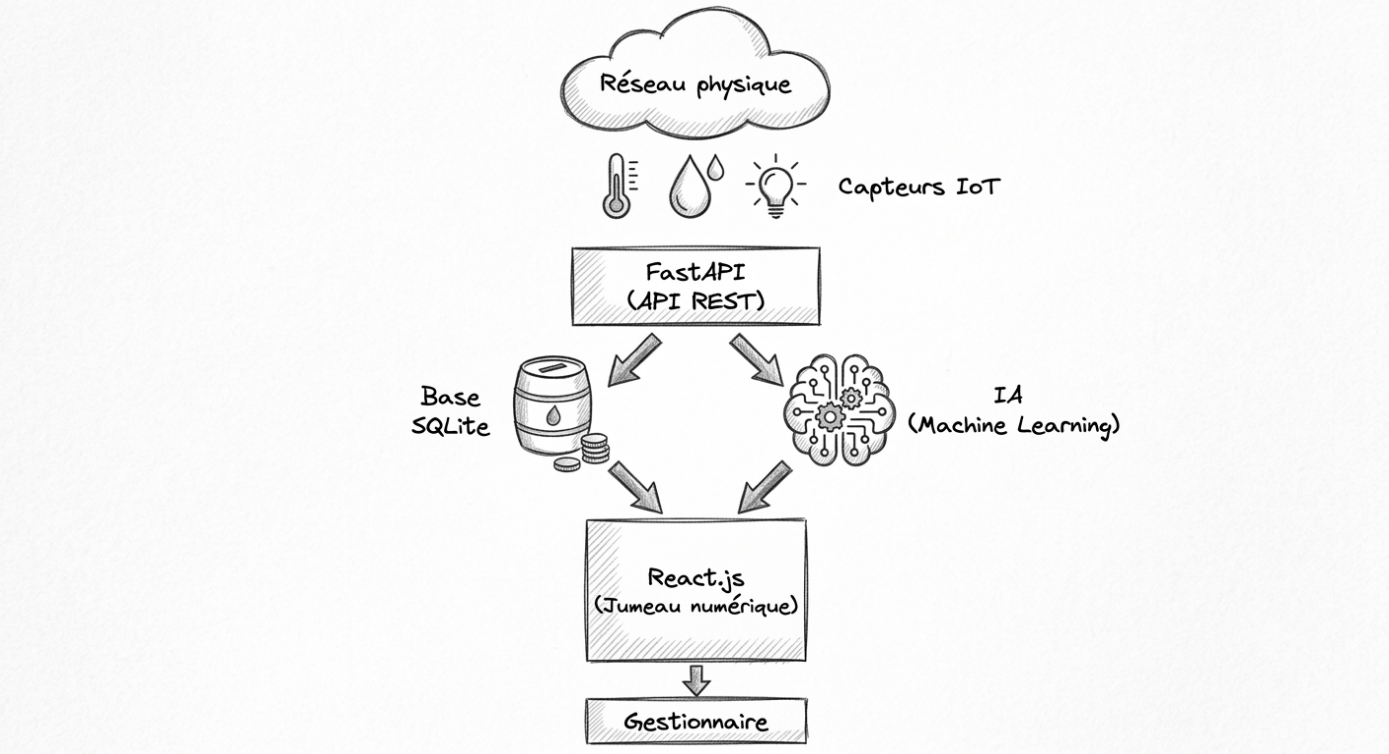
\includegraphics[width=6.3in,height=3.43571in]{figures/image3.png}

Figure 3 Architecture générale du système proposé

3.3.2. Architecture physique

L\textquotesingle architecture physique représente les équipements
matériels intervenant dans le fonctionnement du système.

Elle comprend principalement :

\begin{itemize}
\item
  les infrastructures hydrauliques (réservoirs, conduites, stations de
  pompage) ;
\item
  les capteurs intelligents installés sur le réseau ;
\item
  le serveur hébergeant l\textquotesingle API et la base de données ;
\item
  les ordinateurs utilisés par les gestionnaires ;
\item
  la connexion réseau permettant la communication entre les différents
  composants.
\end{itemize}

Cette architecture garantit une acquisition continue des données du
réseau et leur transmission vers la plateforme numérique pour leur
exploitation \cite{ref20}.

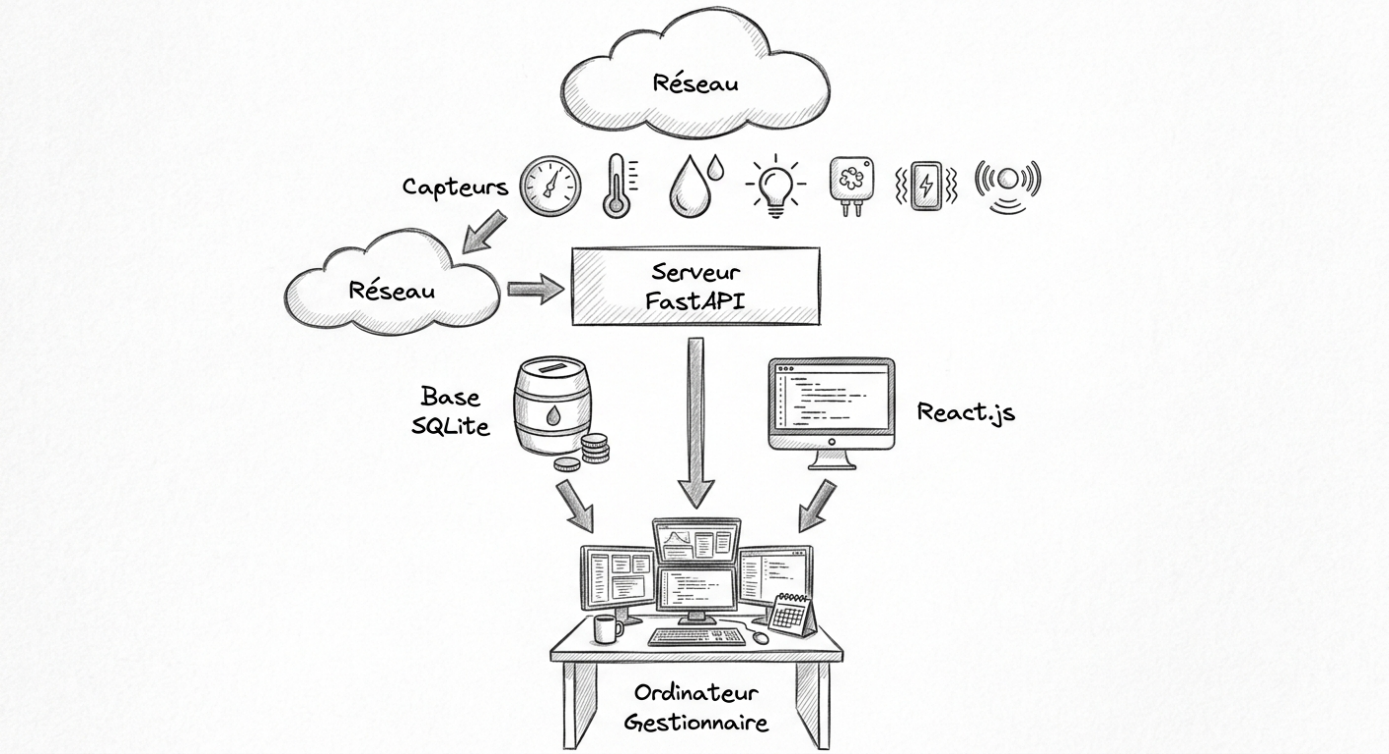
\includegraphics[width=6.3in,height=3.43571in]{figures/image4.png}

Figure 4 Architecture physique

\section{\texorpdfstring{\textbf{3.3.3. Architecture
logicielle}}{3.3.3. Architecture logicielle}}\label{architecture-logicielle}

L\textquotesingle application est développée selon une architecture en
couches (\emph{Layered Architecture}), permettant de séparer clairement
les différentes responsabilités.

Elle est composée de :

\subsubsection{Couche de présentation}\label{couche-de-pruxe9sentation}

Développée avec \textbf{React.js (Vite - JSX)}, cette couche permet aux
utilisateurs de visualiser les informations du réseau, les cartes
interactives, les statistiques et les alertes.

\subsubsection{Couche métier}\label{couche-muxe9tier}

Cette couche est développée avec \textbf{FastAPI}. Elle contient toute
la logique métier, notamment :

\begin{itemize}
\item
  gestion des utilisateurs ;
\item
  gestion des équipements ;
\item
  traitement des données ;
\item
  communication avec l\textquotesingle IA ;
\item
  génération des alertes.
\end{itemize}

\subsubsection{Couche intelligence
artificielle}\label{couche-intelligence-artificielle}

Elle réalise :

\begin{itemize}
\item
  la détection des anomalies ;
\item
  la prédiction des pannes ;
\item
  l\textquotesingle analyse des tendances ;
\item
  les recommandations de maintenance.
\end{itemize}

\subsubsection{Couche données}\label{couche-donnuxe9es}

Cette couche correspond à \textbf{SQLite}, qui stocke :

\begin{itemize}
\item
  utilisateurs ;
\item
  capteurs ;
\item
  équipements ;
\item
  mesures ;
\item
  alertes ;
\item
  historiques.
\end{itemize}

L\textquotesingle utilisation d\textquotesingle une architecture
multicouche améliore la modularité, facilite la maintenance et permet de
faire évoluer indépendamment chaque composant du système \cite{ref106}.

\section{\texorpdfstring{\textbf{3.3.4. Architecture
fonctionnelle}}{3.3.4. Architecture fonctionnelle}}\label{architecture-fonctionnelle}

L\textquotesingle architecture fonctionnelle décrit les principaux
traitements réalisés par le système.

Le fonctionnement général est le suivant :

\begin{enumerate}
\def\labelenumi{\arabic{enumi}.}
\item
  Les capteurs mesurent les paramètres du réseau.
\item
  Les données sont envoyées au serveur FastAPI.
\item
  Les informations sont enregistrées dans la base de données.
\item
  Le moteur d\textquotesingle intelligence artificielle analyse les
  mesures.
\item
  Les anomalies sont détectées.
\item
  Les alertes sont générées.
\item
  Les résultats sont affichés sur le jumeau numérique.
\item
  Les gestionnaires prennent les décisions nécessaires.
\end{enumerate}

Cette organisation garantit une surveillance continue et facilite la
maintenance prédictive du réseau \cite{ref17}.

\section{\texorpdfstring{\textbf{3.3.5. Architecture de
déploiement}}{3.3.5. Architecture de déploiement}}\label{architecture-de-duxe9ploiement}

Le système est conçu selon une architecture client-serveur.

Le serveur héberge :

\begin{itemize}
\item
  FastAPI ;
\item
  SQLite ;
\item
  le modèle d\textquotesingle intelligence artificielle ;
\item
  les API REST.
\end{itemize}

Les clients utilisent simplement un navigateur Web.

L\textquotesingle interface React.js communique avec FastAPI via
\textbf{Axios}, qui envoie des requêtes HTTP pour récupérer ou
transmettre les données.

Cette architecture permet un déploiement aussi bien sur un serveur local
que sur un serveur cloud sans modification majeure de
l\textquotesingle application \cite{ref114}.

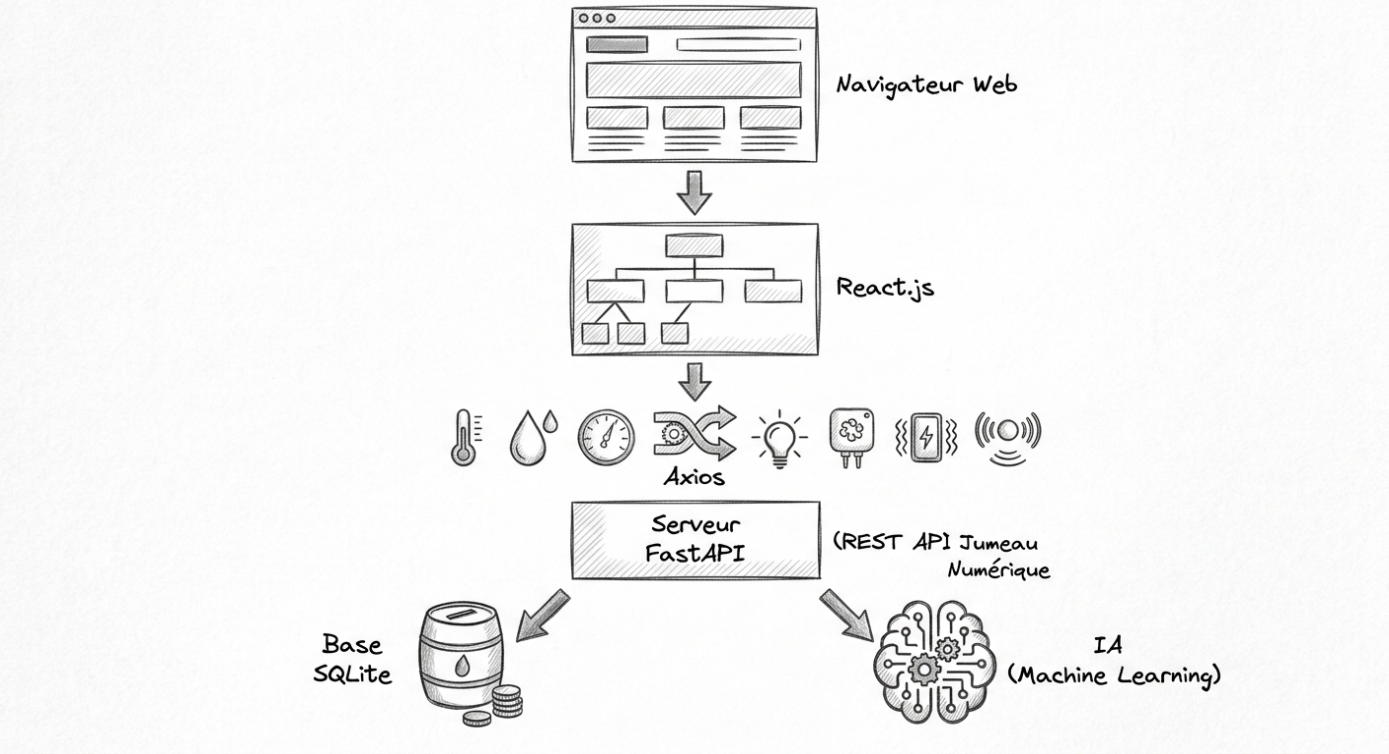
\includegraphics[width=6.3in,height=3.43571in]{figures/image5.png}

Figure 5 Architecture de déploiement


\printbibliography[heading=bibintoc,title={Références bibliographiques}]

\end{document}
